\documentclass[preprint]{aastex}
\usepackage{graphicx}

\newcommand{\code}[1]{\texttt{#1}}
\newcommand{\Fig}[1]{Fig.~\ref{#1}}
\newcommand{\Sec}[1]{Sec.~\ref{#1}}
\newcommand{\Table}[1]{Table~\ref{#1}}
\newcommand{\ticket}[1]{ticket \code{\##1}}
\newcommand{\by}{$\times$}

% -- a @%< hack to redefine placement of abstract in \maketitle
\makeatletter
\def\@maketitle{%
 \newpage
 \begingroup
  \let\footnote\thanks
  \let\email\make@authoremail
  \let\affil\make@affil
  \let\altaffilmark\make@altaffilmark
  \let\altaffiltext\make@altaffiltext
  \let\and\make@and
  \@title
  \@author
  \@date
  \par
  %\@abstract
  \@ifxundefined\keyword@list{}{%
   \expandafter\@keywords
   \expandafter{\keyword@list}%
  }%
 \endgroup
 \clearpage
}%
\makeatother


\shorttitle{LSST Data Challenge 2}
\shortauthors{Axelrod, Becker, Plante et al.}

\DeclareGraphicsExtensions{.pdf,.jpg,.png}

\begin{document}

\title{LSST Data Challenge 2}


% -- Author/Affiliation information
\author{Tim Axelrod, Robyn Allsman, Jeff Kantor, Jon Myers, 
        Francesco Pierfederici}
\affil{LSST Corporation}

\and\author{Serge Monkewicz}
\affil{NASA Infrared Processing and Analysis Center}

\and\author{Greg Daues, David Gehrig, Steve Pietrowicz, Raymond Plante}
\affil{National Center for Supercomputing Applications}

\and\author{Jacek Becla, Kian-Tat Lim}
\affil{Stanford Linear Accelerator Center}

\and\author{Andrew Becker, Lynne Jones, Russell Owen, Nicole Silvestri}
\affil{University of Washington}

\and\author{Robert H. Lupton}
\affil{Princeton University}

\and\author{Jeff Bartels}
\affil{Cirrus Enterprises}

\begin{centering}
\textbf{ABSTRACT}

\begin{quotation}\noindent%
This report describes the second in a series of formal prototypes of
the LSST Data Management System referred to as Data Challenge 2 (DC2).
The focus of this data challenge is integrating real scientific
algorithms that are important to LSST nightly processing into a
general pipeline processing framework and then using the system to
process real astronomical data from a large CCD mosaic.  We enumerate the goals and
metrics for DC2, summarize the architecture of the DC2 pipeline
system, and review the science application and middleware
components that make up the system.  Finally, we present the results
of executing DC2 on data from the CFHT Legacy Survey and highlight the
important conclusions that will be used as input into the next data
challenge.  
\end{quotation}
\end{centering}

\tableofcontents
\clearpage

% -- section 0
\section*{Executive Summary}
\addcontentsline{toc}{section}{Executive Summary}

Data Challenge 2 (DC2) is the second in a series of prototypes of the LSST Data Management System (DMS).  Through these data challenges, we seek to identify the most challenging technical problems to building a DMS that meets the LSST science goals.  We prototype specific solutions to these challenges with the expectation that by the start of the construction phase of the telescope, we will have a well-defined plan for how to build a DMS that can perform at the level needed by first light.  Despite the prototyping nature of the data challenges, we are not producing throw-away code; rather, we expect that the software we produce in the data challenges will serve as the foundation for the DMS that will be completed during the construction phase.

\subsubsection*{Results}

In Data Challenge 1 (DC1), we focused on the DMS middleware design for supporting nightly processing.  In particular, we designed and prototyped the pipeline framework that would host the scientific algorithms used to process the data coming from the telescope.  DC1 did not include actual implementations of scientific algorithms but rather tunable \textit{resource consumers} that simulate the expected computation load of the algorithms.

In DC2, we focused on replacing these simulators with real implementations of the scientific algorithms.  More of our software architecture was refined, including the choice of using C++ to implement compute-intensive components and Python for integrating components, and we built a software development environment.  Consequently, we updated the pipeline framework into this new architecture.  We executed our second-generation nightly pipeline on real astronomical data from the Canada-France-Hawaii Telescope's Legacy Survey.

In all, we developed 49000 lines of C++ in 205 classes and 2330 methods, and 34000 lines of Python in 387 classes and 2111 methods.  The effort was 9 FTE for a year.  This is well above the productivity needed for MREFC development, allowing for increased levels of testing and more stringent performance needed for the production system.

\subsubsection*{Applications}

We developed, unit tested, and executed Image Subtraction, Detection, Moving Object Processing, and Association Pipelines.  All of the pipelines were developed as ``pluggable'' Stages within the Pipeline Harness and used the newly-developed Event system to synchronize.

We executed over 100 runs of the pipelines at various levels of completeness, including several runs at ``full'' scale, i.e.~with all of the processing nodes available. These runs were executed on a small dedicated cluster hosted at NCSA. We have focused our analysis of the results on three particular runs that featured identical versions of the software: \code{rlp0127}, \code{rlp0128}, and \code{rlp0130}.  In these runs, the Image Processing and Detection (IPD) pipeline featured 1 master pipeline process and 36 slice process running across six nodes of the cluster.  The Moving Objects Prediction System (MOPS) pipeline ran on one node with 3 slice processes.  The Association pipeline ran entirely in one process, the master process, on the node where the database was located.

Each of these runs operated on a different set of 36 amplifier-sized images from the same set of mosaic CFHT-LS D4 exposures (amplifier numbers 73--108, 37--72, and 181--214, respectively).  From a total of 288 possible amplifier images per exposure, the amplifier sets were chosen to sample different areas of the focalplane; \Fig{SumFigMegaCamMap} illustrates the location of these amplifier sets.  The number of visits completed in each run were 53, 62, and 62, respectively, for a total of 177 visits.   A summary of the three runs, including the number of images successfully processed, appears in \Table{TSum-1}.  

\begin{figure}[htbp]
\begin{center}
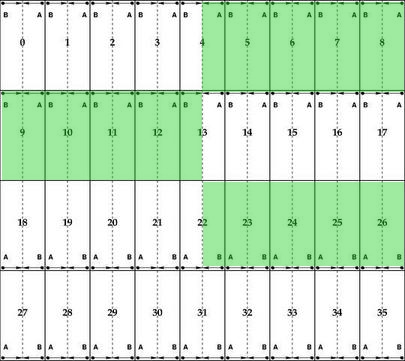
\includegraphics[height=60mm] {figures/MegaCamMap}
\caption{Map of the CFHT MegaCam focalplane.  The area covered by DC2
  runs rlp0127, rlp0128, and rlp0130 are shaded.}
\label{SumFigMegaCamMap}
\end{center}
\end{figure}

\begin{table}[htbp]
\begin{center}
\caption{Summary of DC2 Reference Runs\label{TSum-1}}
\vspace{\baselineskip}
\begin{tabular}{ | r | r | r | c | r | r | r |}
\hline
runId & nVisits & nAmps & Amp IDs & inputImages & outputImages & outputFrac \\ \hline
rlp0127 & 53 &  36 &  73-108 & 1908 & 1875 & 0.983 \\ \hline
rlp0128 & 62 &  36 &  37-72  & 2232 & 2228 & 0.998  \\ \hline
rlp0130 & 62 &  36 & 181-214 & 2232 & 2213 & 0.991 \\ \hline
Total   & --- & 108 &   ---    & 6372 & 6316 & 0.991 \\ \hline
%\hline
\end{tabular}
\end{center}
\end{table}

We note that the DC2 pipeline will run without modification on much larger clusters.  A cluster with 288 cores would allow the full CFHT MegaCam mosaic to be processed in parallel.  We expect such hardware to be available to us very soon, and we will supplement this report with results from such runs when they are available.  We discuss scalability implications for LSST later.

All of these applications extensively reused the object-oriented Application Framework that was developed in DC2. This Framework was designed to standardize astronomical data representations and core functions so that they can be reused in any pipeline.

The goals for the application framework and for the algorithms implemented using it have been nearly completely achieved, and this is clearly one of the major results of DC2.  The prototype nightly processing pipelines include the required algorithms, and have worked reliably as measured by the fraction of input images that are successfully processed through the pipeline.

The one application goal we have not yet achieved is establishing a realistic object/source database for use by the broader collaboration. While we have successfully implemented the database to the schema as designed, and populated it with properly structured and linked data, the data quality is not yet sufficient to be useful to the broader collaboration.  The reasons for this are well understood and described in this report, and much of the application code required to achieve the goal has already been written and tested.  We anticipate achieving this goal fully in the course of Data Challenge 3.

\subsubsection*{Middleware and Infrastructure}

Standard middleware was provided for deploying processing to parallel nodes in a cluster, scheduling the processes, inter-process communication and data transfer, synchronization via events, and for saving data to and retrieving data from FITS files, serialized object files, and relational databases.

The innovation of the newly implemented pipeline harness is in the way it effectively balances to use of Python and C++.  Application Stages --- the container for the scientific algorithms --- can be written with ease in Python.  These stage implementations themselves can be thin wrappers around our C++ classes.  Similarly, the pipeline harness itself is a wrapper around a C++ implementation where the MPI control calls are executed.  Our timing results show that the overhead added to the total processing time by the pipeline harness is very small compared to application processing time.  In particular, the overhead scales linearly with the number of stages ($< 0.1$ seconds per stage) in the absense of event processing.  Sending and receiving events adds additional but still small overhead.  

Our pipeline harness does have a disadvantage that becomes apparent when run on a heterogeneous cluster as we did.  Because of the way we synchronize our processing, the overall speed of the pipeline is limited by the performance of the slowest node.  This is important to consider for the production system.  When we scale up to hundreds or even thousands of cores and run nearly 24 hours a day, one or two defective nodes could easily limit the performance of the entire cluster.  In future data challenges, we will look at strategies for not only minimizing this effect, but also detecting when defective nodes are having a major impact on performance.

\subsubsection*{Development Environment}

We have been quite successful in assembling and configuring an effective software development environment that not only builds the software via a few simple commands but also manages all of the package dependencies.  The ability to have multiple versions of a package simultaneously, as provided by the EUPS system, has been a very powerful feature, particularly during the integration phase when many changes were coming in rapidly.  

Our package distribution system has also been an important mechanism for our distributed team to keep up with the latest changes.  However, the distribution system has suffered from two problems.

First, it has been difficult to ensure smooth installation of third party packages across all of our development platforms.  While the differences between the Mac and Linux platforms have been the most challenging, supporting different distributions of Linux (particularly 64-bit Linux) has not been without problems.

The second problem stems from the amount of time it takes to install a full software stack (as we build everything from source).  This is not only a barrier to new developers but to those of us who maintain the build and distribution system as it makes debugging platform-dependent problems a slow process.  We hope our future experiments with virtual machines will alleviate the barrier for new developers.  

\subsubsection*{Required software developments for DC3}

As we prepare to transition from the completion of DC2 to the development of DC3, it is appropriate to assess what improvements will be required in the existing LSST software.  First, we emphasize that our experience with the DC2 framework, and with the software development system with which it was designed, built, and documented, has been very positive.  We will use it as the foundation for DC3.

As we fully expected, however, we will need to extend it in various ways. The preceding sections of this report have identified a number of detailed improvements to the existing framework classes that we expect to need for DC3.  We will not recap those here, rather taking a somewhat higher level view.  The main required developments that we have identified are:

\begin{itemize}

\item We need to define the role of the middleware orchestration layer in catching exceptions and possibly mediating adaptive behavior of the pipeline stages in recovering from problems such as algorithmic failures.

\item We need to define API and mechanism for inter-slice communication (neither present nor required for DC2).  We have at least three usecases that require some form of inter-slice communication: cross-talk correction; the association pipeline (which is currently using shared memory outside of the pipeline framework for this), and handling Footprints that cross amplifier boundaries.

\item In a related issue, the LSST focalplane --- with its roughly 3000 amplifiers, 200 ccds, and 21 rafts --- has lots of boundaries. We need to carefully assess where processing needs to take account of what's on the other side of a boundary.

\item We need to address the performance issues with accessing pixels under \code{vw}, as described in the next subsection.  This is the source of our only significant performance problem.

\item We need to further develop the image subtraction software to improve the data quality of the subtracted images.

\end{itemize}

\subsubsection*{Scaling to LSST}

Finally, we need to assess where we stand in relation to the final performance requirements for LSST.  The input images we have used for DC2 have 340 Megapixels, just over 10\% the size of the LSST focalplane.  They also have very similar pixel scale and somewhat greater exposure depth as a single LSST exposure.  Although the hardware available for DC2 prevented us from processing full images in parallel, the DC2 software is designed to do so without modification. We expect to make such runs shortly after completion of this report. We are thus very close to processing a data stream that is 10\% that of LSST.  This is in line with the expectations for DC2 set in the MREFC proposal.

We do have a significant shortfall in the per-node performance on the nightly processing pipeline, achieving about 20\% of what is required to meet the 60 sec alert processing latency.  As discussed above, we believe that we have isolated the performance problem to a small section of code that utilizes the Vision Workbench (\code{vw}) library to access image pixels. Our strategy for verifying that we are on track to achieve the full LSST performance level is to:

\begin{itemize} 

\item Complete the full focalplane DC2 runs, utilizing 288 nodes for the IPD pipeline.  This will verify that the middleware framework is not limiting performance. 

\item Work with the \code{vw} group at NASA Ames to resolve the pixel access performance issues that are limiting image subtraction speed. 

\item In the event that \code{vw} continues to be a performance issue, we will replace it.  The application APIs would not be significantly impacted by such a change, so changes to the existing software stack would be very localized. 

\item As a risk reduction strategy, we will continue our ongoing effort to track and evaluate the performance of GPU and related architectures for image processing tasks.  Based on present application experience, these offer at least a factor of 4 improvement in per-node performance, which gives ample headroom to meet full LSST performance. 

\item We need to address load balancing issues inherent to our pipeline harness to ensure that a few defective nodes in a cluster do not drag down the performance of a massively parallel pipeline.   

\end{itemize}

We will have results from the first three steps in this plan by May, 2008.

\clearpage

% -- Section 1
% section 1: Introduction

\section{Introduction}

Data Challenge 2 (DC2) is the second in a series of prototypes of
the LSST Data Management System (DMS).  Through these data challenges,
we seek to identify the most challenging technical problems to
building a DMS that meets the LSST science goals.  We prototype
specific solutions to these challenges with the expectation that by
the start of the construction phase of the telescope, we will have a
well-defined plan for how to build a DMS that can perform at the
level needed by first light.  Despite the prototyping nature of the
data challenges, we are not producing throw-away code; rather, we
expect that the software we produce in the data challenges will serve as
the foundation for the DMS that will be completed during the construction
phase.  

In Data Challenge 1 (DC1), we focused on the DMS middleware design for
supporting nightly processing.  In particular, we designed and
prototyped the pipeline framework that would host the scientific
algorithms used to process the data coming from the telescope.  DC1
did not include actual implementations of scientific algorithms but
rather tunable \emph{resource consumers} that simulate the expected
computation load of the algorithms.  In DC2, we focused on replacing
these simulators with real implementations of the scientific
algorithms.  More of our software architecture was refined, including
the choice of using C++ to implement compute-intensive components and
Python for integrating components, and we built a software development
environment.  Consequently, we updated the pipeline framework into
this new architecture.  We executed our second-generation nightly pipeline
on real astronomical data from the Canada-France-Hawaii Telescope's
Legacy Survey.  
% need DC1 report reference
% need CFHTLS reference http://www.cfht.hawaii.edu/Science/CFHLS/

This report describes the results of Data Challenge 2.  We enumerate
our goals, summarize the implementation, and report on what we've
learned from it.  

\subsection{Goals of DC2}
\label{Goals}

As laid out prior to beginning implementation, the goals of Data
Challenge 2 were to:
\begin{itemize}
\item Demonstrate the use of astronomical algorithms for nightly
  processing in an LSST processing framework.
\item Further develop and demonstrate common application framework
  functionality.
\item Update the middleware implementation to enable the hosting and
  execution of C++ application classes.
\item Establish an LSST simulated object/source database for testing
  by the broader collaboration.
\item Demonstrate a database partitioning scheme.
\item Demonstrate integration of the Moving Objects Prediction
  Software (MOPS) into the LSST framework. 
\item Pilot the software development and testing process for future data
  challenges and the LSST construction phase.
\item Establish a reusable code baseline for future data challenges and
  the LSST construction phase.
\item Test the bandwidth utilization of the UDT protocol in the
  context of LSST data replication between Chile and the US.
\end{itemize}

As of this writing, all but the last goal have been addressed.  This
last goal is part of a now-expanded experiment to test data transfer
tools over long-distance networks.  The results of this work will be
discussed in a subsequent report and therefore will not be discussed
further here.  

\subsection{Metrics and Validation of DC2}

At the start of the DC2, we set down a list of deliverables that we
would need to achieve to validate that we had met our goals.  These
deliverables were:
\begin{itemize}
\item Demonstration of a nightly processing pipeline that operates
  continuously on a set of input data. This processing includes at
  least image subtraction, source detection, association, and moving
  object detection using MOPS. As stretch goals, we would also include
  image linearization (flat-fielding, bias subtraction, etc.) and WCS
  determination.
\item Production of a persistent database of source detections and
  associations as a result of the nightly processing. 
\item Execution of MOPS automatically within the nightly pipeline framework.
\item Management of all original code used in DC2 via our
  Subversion (SVN) repository.
\item Demonstration of the use of LSST framework and support classes.
\item Employment of a harness that accesses MP functionality within a
  compiled layer but which can execute application code via a Python
  interface. 
\end{itemize}

As we describe below, we have in the course of DC2 clearly met the baseline
milestones.  We did not impose formal metrics on the data quality
produced by the astronomical application code in DC2.  We have
nonetheless assessed the data quality, and comment on it in the report sections
that follow.



% -- Section 2
% section 2: Components

\section{Components}\label{sComp}

\subsection{Application Structure}
The production DMS (as described in our reference 
design\footnote{http://dev.lsstcorp.org/model/LSSTModel.pdf}) will
contain three pipeline-processing systems which we refer to as
\textit{multi-pipelines}.  A multi-pipeline is a set of one or more
loosely-coupled pipelines that coordinate to create a set of related
data products.  The three multi-pipelines, illustrated in
\Fig{fComp-pipe}, divide their responsibilities between nightly
processing, calibration products, and data release processing.  DC2 is
intended specifically to prototype the nightly processing pipeline.
The full structure of this pipeline as intended for the production DMS
is shown in more detail in \Fig{fComp-nite}.  DC2 implements
the ``backbone'' of the nightly processing flow; illustrated in
\Fig{fComp-dc2}, it includes:

\begin{itemize}
\item Image subtraction;
\item Source detection;
\item Association of Sources to Objects; and
\item The ``night'' portion of the Moving Objects Prediction Software
  (MOPS), which calculates predicted positions of known solar system
  objects in the incoming exposures.
\end{itemize}

As can be seen in part from a comparison of \Fig{fComp-nite} and
\Fig{fComp-dc2}, several aspects of the full LSST nightly processing were
not included in DC2: 

\begin{itemize}
\item Instrumental signature removal stage of the image processing
  pipeline (debiasing, flatfielding, etc.);
\item Alert processing;
\item The ``day'' portion of MOPS, which links together detections
  into tracks, and determines orbits; and
\item Combined processing of the two exposures which make up a single
  visit. The DC2 input data (\Sec{sInDat}) was not taken with the
  required cadence to allow this.
\end{itemize}

\begin{figure}[htbp]
\begin{center}
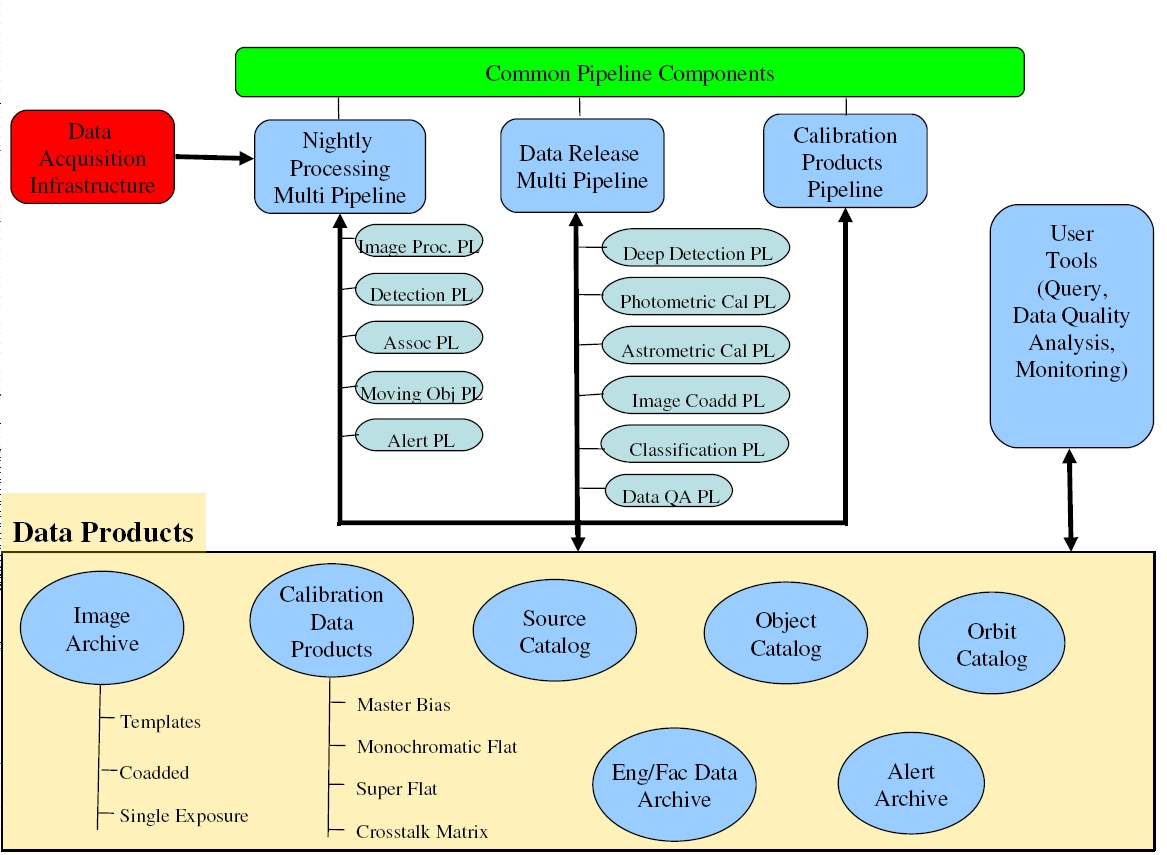
\includegraphics[height=0.45\textheight] {figures/LSSTPipelines}
\caption{The LSST Data Management Pipelines\label{fComp-pipe}}
\end{center}
\end{figure}

\begin{figure}[htbp]
\begin{center}
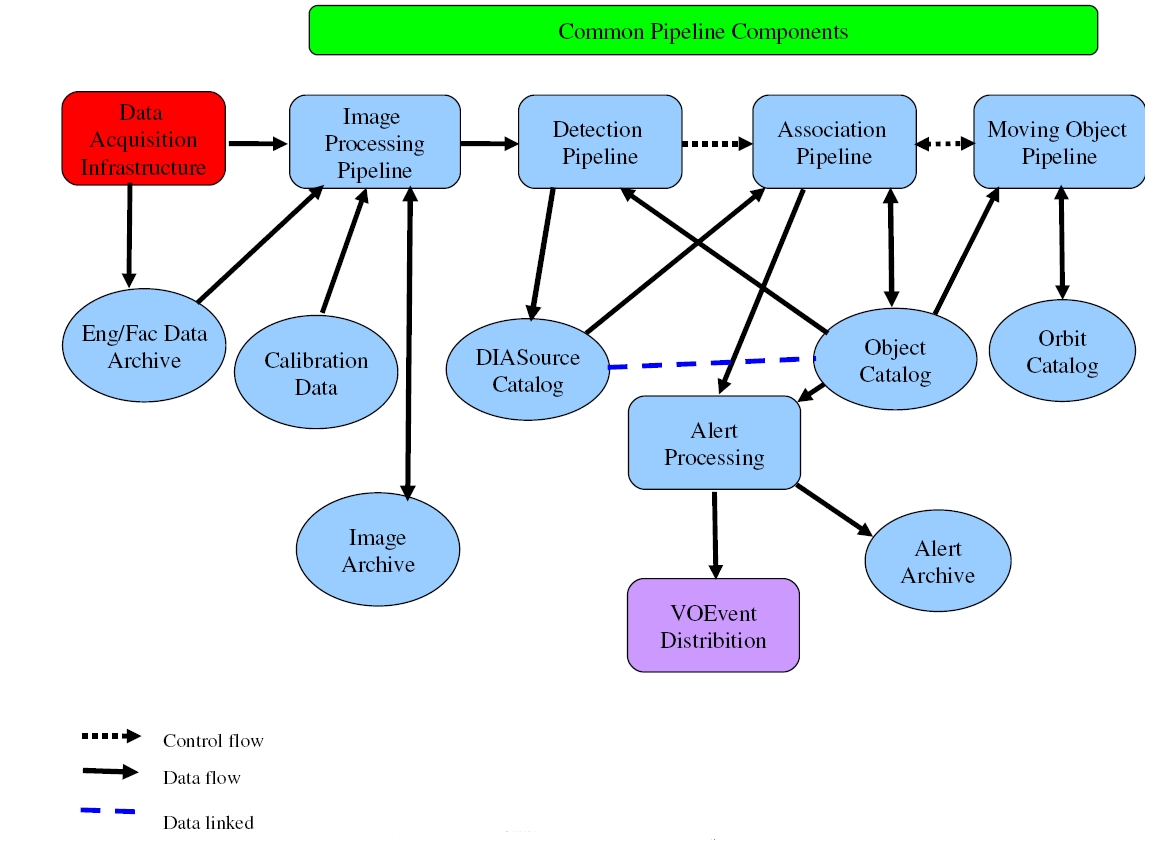
\includegraphics[height=0.45\textheight] {figures/LSSTNightlyPipeline}
\caption{The LSST Nightly Pipelines\label{fComp-nite}}

\vspace{0.05\textheight}

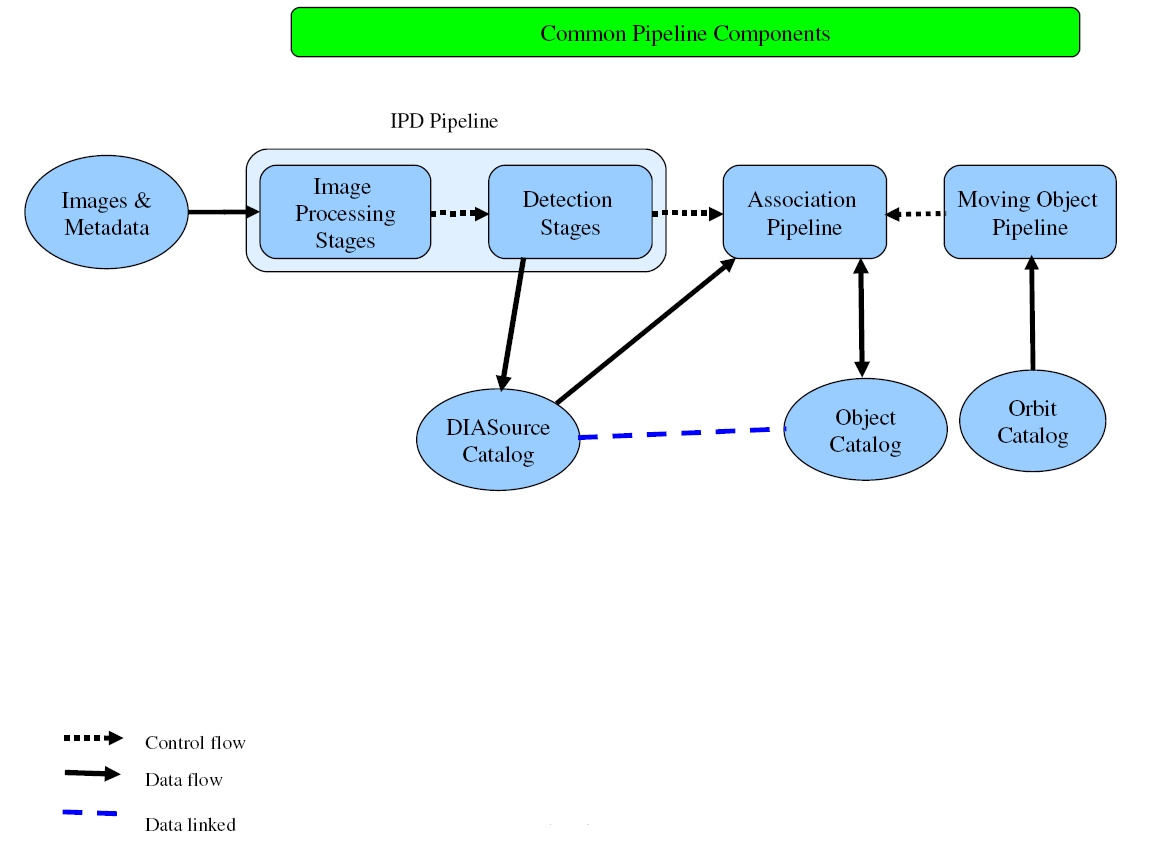
\includegraphics[height=0.45\textheight] {figures/DC2Pipelines}
\caption{The DC2 Pipelines\label{fComp-dc2}}
\end{center}
\end{figure}

The DC2 system is functionally comprised of three separate pipelines:
the Image Processing and Detection (IPD) pipeline, the Moving Object
(MOPS) pipeline, and the Association pipeline.  (Although the Image
Processing and Detection pipelines are logically separate pipelines in
our design, we have implemented them in our software framework as
stages within a single functional pipeline.  This choice does not
change the logic of the applications flow, but increases the execution
efficiency, since the images being transferred between Image
Processing and Detection can remain in memory without consuming I/O
resources.)  The three pipelines are loosely coupled via event-based
communication (\Sec{sMw-ev}).  They also share access to a
MySQL\footnote{http://www.mysql.com} database.  An early prototype of the pipeline
orchestration layer (\Sec{sMw-orc}) is responsible for deploying
the multi-pipeline to a cluster, executing it, and feeding it its
input data.  The whole system is configured via a set of so-called
\textit{policy files}.  These define the different stages that make up
the pipelines and provide values for parameters that control the behavior
of components.

\subsection{Summary of Processing Flow}\label{sComp-flo}

The DC2 multi-pipeline is executed via the orchestration layer
(\Sec{sMw-orc}) which is represented by the \code{dc2pipe} software
package.  Before actually starting the pipelines, the operator usually
configures the pipeline by making a copy of the default policies for
the particular flavor of pipeline being run (found in a repository
that is part of the \code{dc2pipe}) and then altering the values as
desired.  Among the configuration parameters that can be set are the machines that
will be used, the number of parallel processes that will be employed,
and the subset of CCDs making up each observed mosaic that should be
processed.  A separate file lists the sequence of exposures (which we
refer to as \textit{visits}) that the pipelines will operate on.
Normally, the operator uses one of a few default lists provided by the
\code{dc2pipe} package, but the file can be altered as desired.

\begin{table}[htbp]
\begin{center}
\caption{Summary of the stages composing the nightly pipelines\label{tComp-stg}}
\vspace{\baselineskip}
\begin{tabular}{|cp{0.85\textwidth}|}
\tableline
\multicolumn{2}{|l|}{Image Processing and Detection (IPD)} \\
  1 & Create links to the visit's input images in the run's filesystem 
      sandbox. \\
  2 & Load the visit's input images into memory. \\
  3 & Transform the visit's metadata. \\
  4 & Record the visit's metadata in the database. \\
  5 & Write out a copy of the input image data. \\
  6 & Subtract the input images. \\
  7 & Write out the difference image. \\
  8 & Detect sources in the difference image. \\
  9 & Record the detected sources into the database's DIASource catalog. \\
 10 & Send an event to the association pipeline indicating that
      detections are ready. \\
\tableline
\multicolumn{2}{|l|}{Moving Object Processing (MOPS)} \\
  1 & Load visit-specific data into memory.  (Currently no such data
      is being loaded.) \\
  2 & Predict the locations of known moving objects in the field. \\
  3 & Record the predicted positions into the database. \\
  4 & Send an event to the association pipeline indicating that
      predictions are available. \\
\tableline
\multicolumn{2}{|l|}{Association} \\
  1 & Load the Object catalog for the relevant sky region into memory. \\
  2 & Load new source detections from the DIASource catalog into memory. \\
  3 & Match the detections against known, non-moving objects. \\
  4 & Record matched sources into the database.  \\
  5 & Load new MOPS predictions into memory. \\
  6 & Match the detections against known, moving objects.  \\
  7 & Record the matched sources into the database.  \\
  8 & Update historical knowledge of the sky.  \\
\tableline
\end{tabular}
\end{center}
\end{table}

Once the system is configured, the operator starts it via a script 
(\code{launchDC2.py}) which deploys the pipelines on the proper
machines.  One important input to this script is an identifier
referred to as a \textit{run-ID}.  This is used to set up ``sandboxes''
on the file system and in the database where data related to this
particular execution --- or \textit{run} --- of the pipeline can be collected
and kept separate from other pipeline runs.  After the sandboxes are
set up, the pipeline processes are started on the proper machines which,
after some initialization, pause to await the arrival of new data to
process.  

New data is sent to the pipelines by the orchestration layer via a
sequence of event messages.  These messages are constructed in DC2 from
the information found in the file containing the list of visits, a
role that will be played by the Camera data acquisition interface on
the production LSST.  For
each visit, the information includes a visit identifier, the filter
that was used during the visit, and the sky position for the center of
that field.  The visit events are delivered in sequence to both the
IPD and MOPS pipelines, and the first stage of each processes them in
order.  The MOPS pipeline uses the field position to calculate the
predicted positions within the field of known moving objects.  The IPD
uses the visit information to find the next calibrated exposure along
with the associated template images and load them into memory.  

Each pipeline is composed of a sequence of \textit{stages}
(\Sec{sMw-har}).  Data are passed through the stages via a set of 
data queues that stitch the stages together.  Pipelines can coordinate
their activities by sending and receiving event messages.
Table~\ref{tComp-stg} summarizes the function of each stage in each of the
three pipelines.  

In summary, the IPD pipeline first loads the input images into memory.
It next applies the image subtraction algorithm (\Sec{sApp-imsub}) to
produce a difference image.  The detection stage then extracts sources
present in the difference image; these sources represent new objects,
objects that vary in brightness, moving objects, or possibly artifacts
such as cosmic rays.  Descriptions of
these detected sources are stored in the DIASource catalog within the
database.   At the end of the IPD pipeline, it sends an event to the
Association pipeline to tell it that new source detections are
available in the database.  The IPD pipeline then returns to its first
stage and begins operating on the next visit in the input queue.

Meanwhile, as the IPD is processing a visit, the MOPS processes the
same visit in parallel.  It uses the Orbit Catalog to predict the
positions of known moving objects that should appear in the visit's
field of view at the time of its observation.  These predicted
positions are also stored in the database.  The last stage of the
pipeline sends an event to the Association pipeline indicating that
the predicted positions are available.  The MOPS pipeline then returns
to its first stage to process the next field of view.   

The Association pipeline first waits for the event from the IPD
pipeline indicating that new source detections are available for
processing.  It reads the detections from the database and tries to
match them against known (stationary) objects in the Object Catalog.
For those sources that do not yet match known objects, the Association
pipeline uses the event from the MOPS pipeline to match them against
known moving objects.  The DIASource and Object catalogs are updated
to record the matched and unmatched source detections.  At this point, 
the nightly processing for a visit is complete.  

\subsection{The Deployment of DC2 onto Hardware}\label{sComp-hw}

The DC2 pipelines ran on a small, dedicated cluster located at NCSA
comprised of ten Dell Server blades with Xeon processors.  Four of the
blades are of an older model acquired from a past project and
featuring an earlier model processor with fewer cores per node than
the rest of the cluster; the remaining six are identical blades
feature dual, quad-core processors.  \Table{tComp-hw} summarizes
the processor configuration for the ten nodes.  All the nodes feature
4 GB of RAM except node 10, which has 16 GB.  This node was configured
to host the database, which needs the extra memory for handling very
large tables.  All nodes run 32-bit Red Hat Enterprise Linux AS
Release 4. 

Each node features a modest amount of local disk to hold the OS with
about $~50$ GB available potentially for storing local pipeline data.
Node 10 features a locally-mounted 280 GB filesystem for storing the
database data.  Approximately 750 GB of SAN-based storage (with
optical fiber connects) are available as shared, cross-mounted
filesystems (i.e.~available to all nodes), hosting the LSST software
stack, the repository of input data, and the pipeline run sandboxes.
Originally, this was mounted as a Lustre filesystem, providing
redundant, parallel I/O capabilities to the pipeline.  In this
configuration, the older nodes 1--4 were set up to be used exclusively
as file server nodes.  However, our deployment of the Lustre
filesystem proved unstable, and we were forced to replace this with an
NFS-mounted filesystem.  The expected performance penalties for
NFS did appear
to affect the overall performance of the pipelines, particularly in 
the Association pipeline.

\begin{table}[tb]
\begin{center}
\caption{Hardware summary for the DC2 cluster\label{tComp-hw}}
\begin{tabular}{ccccl}
%\multicolumn{5}{c}{Table \ref{tComp-hw}.  Hardware summary for the DC2 cluster}\\
\multicolumn{5}{c}{\phantom{Hardware summary for the DC2 cluster}}\\
\tableline\tableline
Node & No. of processors & Cores per processor & Memory (GB) & Pipeline hosted \\
\tableline
 1  & 2 & 2 & 4 & IPD \\
 2  & 2 & 2 & 4 & \textit{unavailable}\tablenotemark{a} \\
 3  & 1 & 2 & 4 & \textit{unavailable}\tablenotemark{a} \\
 4  & 1 & 2 & 4 & IPD \\
5-8 & 2 & 4 & 4 & IPD \\
 9  & 2 & 4 & 4 & MOPS \\
 10 & 2 & 4 &16 & Association \\
\tableline
\\[0.5\baselineskip]
\multicolumn{5}{p{0.85\textwidth}}{$^{\rm a}$Hardware and system configuration
  issues made these nodes too unstable for consistent use as pipeline nodes.}\\
\end{tabular}
\end{center}
\end{table}

As shown in Table~\ref{tComp-hw}, the three pipelines were completely
segregated on different sets of nodes.  (The segregation is actually a
constraint imposed by our use of MPI.)  Because of its heavy use of
the database, the Association pipeline was deployed onto node 10.
Though this pipeline is singly-threaded, the remaining compute 
resources were reserved for use by database processes.  The MOPS
pipeline ran with 4 total processes on node 9.  The remaining
available nodes were used to host the IPD pipeline; one process per
available processing core was deployed on each node.  



% -- Section 3
% section X: Input Data

\section{Input Data}
\label{sInDat}

\subsection{Input Images}

As part of our long-term strategy for our data challenges, we have
intended to apply our software to both simulated LSST images and real
mosaic images from existing telescopes.  While the former category
allows to ensure we meet the requirements imposed by our own telescope
and data acquisition system, the latter is important for two reasons.
First, real data forces us to deal with real-world observational
artifacts and the unexpected consequences they present.  Second, we
hope that by operating on a variety of existing data, our software will retain
sufficient generality that many of the components will be useful
outside the context of LSST.  

At this time we do not have simulated images that are sufficient for
validating science pipelines; thus, in DC2, we focused on two existing
datasets that are similar to what we expect to get from LSST.  Both of
these datasets come from the Canadian-France-Hawaii Telescope (CFHT)
using the MegaCam mosaicing camera.  This camera features a focalplane 
of 36 2048 \by\ 4612 pixel CCDs (a total of 340 megapixels),
covering a full 1 degree \by\ 1 degree field-of-view with a resolution of
0.187 arcsecond per pixel.  As discussed below in \Sec{sInDat-t}, we
approximate the images that the LSST camera will be delivering to the
DMS by dividing each CFHT CCD into 8 1056 \by\ 1161 pixel sections for a
total of 288 images, each closely equivalent in the number of pixels
to the images produced by the individual amplifiers of the LSST
camera.  By comparison, the LSST camera will contain 189 CCDs, each
with 16 2000 \by\ 500 amplifier sections, for a total of 3024 outputs.
So, in the form we have prepared it, the CFHT Megacam data is roughly
10\% of both the number of amplifiers and the number of pixels
possessed by LSST.

The first of the two datasets we selected comes from the CFHT Legacy
Survey (CFHT-LS)\footnote{http://www.cfht.hawaii.edu/Science/CFHLS/}.
This survey had three parts to it: two wide and
shallow, and one deep.  In the ``deep'' survey, the CFHT-LS
team chose four 1 square-degree fields that were observed repeatedly
to obtain up to 132 hours of integration time across 5 filter bands
for high sensitivity to the dimmest galaxies.  The availability of
repeated exposures of the same field made this a particularly good
choice as an LSST pre-cursor dataset.  In particular, we chose to use
the so-called \textit{D4} field because of its close proximity to the
ecliptic.  The increased chance of detecting solar system objects
provided by this field allows us to exercise our MOPS pipeline.  

The second dataset we chose was the Thousand Asteroid Light Curve
Survey 
(TALCS)\footnote{http://irtfweb.ifa.hawaii.edu/~sjb/CD07/abstracts/Masiero.CTabs.pdf}. 
This survey is producing repeated observations
of asteroids that can be used to measure their light curves.
Consequently, this is an even better set for exercising MOPS.
However, because of minor complications in acquiring and preparing the
TALCS data, we were not able to incorporate the data in time for DC2.
Nevertheless, we expect to use this data in DC3.  

\subsection{Preparing the CFHT-LS Deep Data}\label{tInDat-prep}

As described in the previous section, the Image Processing and Detection pipeline
focuses on the image subtraction as input to the detection of new,
variable, and moving sources.  Thus, to use the CFHT-LS Deep data in
DC2, we needed (a) calibrated mosaic images of each exposure of
the field and (b) a deep, stacked image of the field to
represent the static sky.  Both of these are available from the
CFHT-LS archive.  As a pre-processing step for DC2 (that is, prior to
presenting the data as input to the pipelines), we resampled the
stacked image to the observational footprint of each calibrated mosaic
we planned to process; we refer to these resampled images as
\textit{template images}.  

\subsubsection{Creation of Template Images}\label{sInDat-t}

We downloaded the stacked images of the D4 field in the R and
I-band, D4.2007B.R.fits and D4.2007B.I.fits.  These were used to
derive the template images for the Image Subtraction portion
(\Sec{ImageSubtraction}) of the DC2 pipeline.  The process of
creating these template images proceeded as follows.

Every nightly science image is represented by a \code{.fits} file,
obtained from the CFHT-LS archive, and an associated \code{.head}
file, obtained directly from Stephen Gwyn, a member of the CFHT-LS and
the person responsible for creating the stacked images.  The
\code{.head} files contain updated astrometric information not
available in the \code{.fits} header.  These \code{.head} files were
produced during creation of the stacked images, and result from
running the program
\code{Scamp}\footnote{http://terapix.iap.fr/soft/scamp}.  \code{Scamp}
solves for a common cubic order focalplane distortion (\code{PVn\_n}
keywords) from an ensemble of input images, as well as the pointing,
scale, and rotation of each individual science image (\code{CRPIXn},
\code{CRVALn} and \code{CDn\_n} keywords).  These non-linear terms
were essential for aligning the stacked image with each science image
to sub-pixel levels.

We extracted the header information associated with each of the 36
CCDs in the CFHT focalplane from each science image's \code{.head}
file.  This would serve as the reference astrometric coordinate system
that we warp the stacked image to, yielding the template.  We next
used the program
\code{Swarp}\footnote{http://terapix.iap.fr/soft/swarp} to extract
\textit{only} that portion of the stacked image that overlapped with
the coordinate system defined in the \code{.head} file.  In addition,
the flux was resampled within this window to align exactly with the
science image, yielding a template image aligned at the subpixel
level.  The header files suggest that the internal RMS of the solution
is $0.1\arcsec$, with an external RMS of approximately $0.3\arcsec$.
%
% TSA comment:  do we want to say anything about the small number
% of realy large alignment failures?
%
The resulting fits files were 4644 by 2112 pixels in size.  Since we
expect to operate on $2k \times 0.5k$ images for LSST, we further
subdivided the images into eight $1k \times 1k$ subimages to more
accurately simulate LSST operations.

\subsubsection{Creation of Variance and Mask Images}\label{tInDat-vm}

Each image containing the pixel information was renamed with the
extension \code{\_img.fits} to conform to the \code{MaskedImage}
formalism.  We then synthesized variance (\code{\_var.fits}) and mask
images (\code{\_msk.fits}).  For the template, we made the assumption
that the image was noise-free and contained no masked pixels, so the
variance and mask images were all zero-valued.  For the science
image, we synthesized its variance by dividing the science pixels by
the \code{GAIN} value from the image header (effectively ignoring the
readnoise, which averages $\sim 5$ electrons).  For its mask, we
extracted the \code{SATURATE} value from the image header, and masked
all pixels within 95\% of this value.  This was sufficient for masking
the majority (but not all; see
\Sec{ImageSubtraction-Performance}) of saturated pixels.  For
both the template and science image's mask, we added aligned mask
planes for ``bad'' (\code{MP\_BAD=0}), ``saturated'' (\code{MP\_SAT=1}),
``interpolated'' (\code{MP\_INTRP=2}), ``cosmic ray'' (\code{MP\_CR=3}),
and ``edge'' (\code{MP\_EDGE=0}) pixels.  In the step above, we set
both the \code{MP\_BAD} and \code{MP\_SAT} bits.

\subsection{Input Object Catalog}

The Input Object Catalog was prepared using data from D4 catalog,
detections from R and I bands were used (files D4.2007B.R.cat and 
D4.2007B.I.cat). Detections from these two files were associated
using the procedure documented 
elsewhere\footnote{http://lsstdev.ncsa.uiuc.edu/trac/wiki/dbD4ObjectCatalog}.
Objects were created for each pair of detections, and for the remaining 
unmatched detections. The total number of created objects was 450,000
and the total size was 1 GB.

\subsection{Input Orbit Catalog}

The Moving Objects Pipeline uses a catalog of orbits for known solar
system objects as one of its inputs.  In the production system, the
catalog would respresent our most up-to-date knowledge of the solar
system object orbits as computed by the special-purpose pipeline known
as \textit{DayMOPS} (\Sec{sApps-mops}) that runs each day to incorporate
the previous night's moving object detections into the orbit
calculations.  For DC2, we used a pre-computed object catalog
generated by feeding the the Minor Planets Center 
catalogue\footnote{http://cfa-www.harvard.edu/iau/mpc.html} into
the DayMOPS software.



% -- Section 4
\section{Software Framework}

Our software framework is the toolbox with which we've been able
construct a working DC2 components.  It starts with a software
development environment which includes tools and processes for design
and implementation of the code as well as system for compiling the
code into libraries in a consistant manner that accounts for all the
component interdependencies.  In this environment we have built up set
of reusable components that allow us to implement the scientific
algorithms.  These include components that provide access to
middleware capabilities ({\tt mwi}).  It also includes data structures
(such as an \code{Image}) central to building algorithm
implimentations as well as databases and database services.  Finally,
framework provides a middleware necessary for running pipelines.  At
the center of this is the pipeline framework for creating and
executing pipelines.  Also supporting pipelnes is the event-based
communication layer and the \textit{pipeline orchestration} layer used
for setting up and launching pipelines. 

% Subsection 3.4: build

\subsection{Software Development Environment}

\subsubsection{Design and Development Process}

Software design and development has been guided throughout the LSST project by
standard, established methodologies for large-scale software
development. These same methodologies were also applied in DC2. We highlight two
here.

\paragraph{Determining Requirements Through Use Case}

The starting point for determining the scope of DC2 was the DC2 use case, a
scenario describing the path through the LSST software taken by a single
``visit,'' one particular astronomical exposure, as it goes through the various
stages of processing --- image subtraction, source detection, object
association, and moving object detection.

The LSST DC2 use case was collaboratively developed by members of the LSST Data
Management 
team\footnote{http://dev.lsstcorp.org/trac/wiki/DC2NightlyProcessingUsecase}.
Software requirements for DC2 were in turn derived from this use case; whatever
infrastructure or tools necessary to accomplish this use case was a requirement
for the DC2 software.

\paragraph{UML model and DC2 specialization}

One of the most dangerous traps in software development is trying to hit a
moving target. Adding new features or additional technologies during the
development process may improve the target, but it also moves it. By analyzing
the project requirements in detail up front and capturing the results of that
analysis, the development process can be protected against ``mission creep,'' in
which an ever-moving goal results in an endless development phase.

Software classes for LSST are designed in UML, the Unified Modeling Language, a
general-purpose modeling language for diagramming object specifications. There
is a general LSST model meant for the final production code, and specializations
of that model for specific subgoals such as DC2. The model then guides the
software development. The software design, and its representation in UML, is not
absolutely frozen after the design phase, however; there is some necessary
degree of give and take between the model and its implementation.

The UML model was created and is maintained using a commercial software package,
Enterprise Architect\footnote{http://www.sparxsystems.com.au/} allowing for the
interactive and collaborative design of the model. Enterprise Architect also can
 --- with a little persuasion --- reverse engineer source code into the UML
model, meaning that the code and the model remain synchronized, keeping the
model relevant while discouraging mass \textit{ad hoc} changes to the design.

\subsubsection{The Role of Software Languages}

As a project, we have chosen an object-oriented approach to software
design, and so our choice of software languages for implementing the
DMS reflects this.  We have identified three languages to be used for
developing DMS code.  The vast majority of our code is to be
implemented in C++, particularly the most compute-intensive
components, so as to take advantage of the performance capabilities of
a compiled language.  Python is intended for glueing together C++
components into pipelines.  Java is expected to be useful for
developing user interfaces as well as aspects of control systems where
we can take advantage of existing middleware technologies.  

In DC2, the vast majority of the code --- in particular, all of the code
that makes up nightly pipelines --- was implemented in C++ and Python.
For the Event System (\Sec{sMw-ev}), we adopted the widely-used Java
Messaging system.  Consequently, a small amount of event-handling code
for loading logging event data into a database was written in Java.

C++ classes are made availabie in Python through the use of SWIG, a
tool for creating bindings layers between C/C++ and various other
languages.  For the most part this has worked exceedingly well:  while
many of us as developers have expressed that the SWIG configuration
files (the file that controls which and how C++ classes and functions
are exposed to Python) have the feel of black magic, the result
provides a fully featured interface that is convenient to use.  One
challenge has been SWIG's support for C++ shared pointers
(\code{boost::shared\_ptr}) and getting Python to properly handle
garbage collection of the objects they point to.  For DC2, we found
work-arounds sufficient to achieve our immediate goals.  We have also
been in conversation with the SWIG development team which has resulted
in improved support for shared pointers; we will take advantage of
this in DC3.  
  
\subsubsection{Coding and Documentation Standards}

Software developers on the LSST project are asked to ensure their source code
meets a set of mutually agreed-upon standards for uniform coding practices and
documentation. These standards, derived and adapted from respected open source
best-practices guides, aid the software development process in many significant
ways, reflecting as they do the consolidated, accumulated programming experience
of leaders of the open source development movement.

\paragraph{Coding Standards}

An important principle guiding coding standards is the recognition that a
developer's source code is read by two very different kinds of creature: the
language compiler/interpreter grinding through it, and the human being
extending, modifying, or debugging it. In a geographically distributed
development environment like LSST, our source code must be more self-explanatory
than might be necessary were the developer always sitting a short walk down the
hallway. This is why the LSST standards cover not only technical facets of
language usage but also how the code is documented. These standards were
developed not to enforce consistency for consistency's sake, but to support code
as self-explanatory as possible. Given the long life cycle of the LSST project,
this clarity will also become important should the code need to be modified by
other programmers at a later date to take advantage of new technologies or new
algorithms --- a very likely development.

Other coding standards take the form of recommended programming idioms, such as
the convention that variables should be initialized on the same line on which
they are declared. The advantages of such a convention are two-fold. From the
computer's perspective, it helps guard against inadvertently using an
uninitialized variable. From the human perspective, it prevents a long search,
when reading or modifying the source code, for the line within a function in
which the initialization actually occurs.

The LSST coding standards are posted for reference on the LSST development Trac
Wiki (described in more detail below)%
\footnote{http://lsstdev.ncsa.uiuc.edu/trac/wiki/CodeStandards}. The LSST C++
coding standard represents an amalgamation of standards collected from several
guides to best practices in C++. The LSST Python coding standards are largely
based on those proposed by Guido van Rossum, the creator of the Python language.

A representative example of a Python guideline that might appear overly pedantic
is the recommendation not to mix spaces and tabs when indenting, a distinction
literally invisible in most text editors. There is a simple reason behind this
suggestion, however: since the level of indentation carries semantic value in
Python, a mixture of tabs and spaces for indentation can confuse the Python
interpreter about how far a given line is intended to be indented. By sticking
to the coding standards' proclamation ``Never mix tabs and spaces,'' this
invisible source of potential error is eliminated.

\paragraph{Documentation Standards}
\label{build_docs}

The project has standardized on 
\code{doxygen}\footnote{http://www.stack.nl/\~{}dimitri/doxygen},
an open-source documentation
generator capable of extracting specially marked comments from C++ and Python
source code and generating cleanly formatted documentation in either \LaTeX\ or
HTML format. Keeping the documentation embedded inside the relevant source files
helps keep the documentation synchronized with the source code it documents.


LSST documentation standards indicate that each of the following must be
documented in a format \code{doxygen} can recognize:

\begin{itemize}

\item{Every C++ source and header file (\code{.cc}, \code{.h}) and Python file
    (\code{.py});}

\item{Every C++ and Python class specification, documenting its purpose,
    constructors, public instance variables, and public methods;}

\item{Every supporting function defined outside a class or object specification.}

\end{itemize}

\paragraph{Testing}

Our coding standards call for the creation of unit tests for all
software components as part of the common development process.  In
DC2, we obtained at least partial coverage of our code by unit tests
(enough to demonstrate on a number of occasions the critical value to
maintaining a large code base).  Most of the unit tests were created
against the Python class interfaces using the standard Python package
\code{unittest}, though some are written in C++ (using an ad hoc
testing pattern, as opposed to a formal testing framework) to test
lower level C++ interfaces directly.  In DC3 we plan to migrate our
C++ tests to the framework provided by \code{boost::test}.  

\paragraph{Formal Code Review}

DC2 had a formal process of code review, in which LSST developers would inspect
the code of other members, looking for general comments and also for compliance
to LSST coding standards. Pragmatically, in the last months of development, the
code reviews took a back seat, with the result that in some cases these reviews
were indefinitely postponed as developer time became scarce. For DC3, we will
ensure that code reviews are given equal priority with other development tasks
so that they don't fade away as the DC3 runs approach.

\subsubsection{Open Source Tools}

\paragraph{Description and Usage}
Where possible, LSST uses pre-existing open source software components, not only
in the code itself but also as part of the development environment. Several
robust open-source development tools play a central role in the LSST development
environment. These tools are hosted on a designated server,
\code{dev.lsstcorp.org}, which is located at NCSA.

\paragraph{Trac} Trac\footnote{http://trac.edgewall.org} is a web-browser-based
issue tracking system and wiki designed for managing software development
projects. It gives the LSST team several tools:

\begin{itemize} \item{\textbf{Issue Tracker.} Trac provides a system in which a
given software issue --- a code defect, a needed enhancement, etc. --- is
assigned a ``ticket,'' a record in the Trac database which serves as an
accumulating point for information about the issue and its current status. Each
ticket is assigned to a specific team member, who is responsible for bringing
that ticket's issue to closure. The ticket describes the defect or enhancement,
how to replicate the error, and other relevant information; other team members
can add additional information and comments. Users can call up, via canned
database queries, summaries of their tickets' status or other related
information.}

\item{\textbf{Wiki.} Trac also contains an embedded system of wiki pages,
providing an easily updated set of project web pages. 
The wiki pages are automatically indexed and 
searchable.}

\item{\textbf{Code Browser.} Trac interfaces directly with the Subversion
repository described below, allowing a quick overview of a software component.
Users can drill down to a given file in the repository and browse its current
form, or compare it with a previous revision number with differences
automatically highlighted.}

These tools are tightly integrated; for example, a user can easily indicate
a ticket number on a wiki page, and a link will automatically be created 
to the relevant ticket. The link text will appear as strike-through if the
ticket has been resolved. This allows a developer to quickly access 
the code and related documentation in wiki format. 

\end{itemize}

\paragraph{Subversion} Subversion\footnote{http://subversion.tigris.org}
is a source code version control system.
It provides a curated library for LSST source code and related documents,
maintaining a revision number for every document a programmer registers with
(``checks into'') the Subversion repository. Subversion can also recreate
previous versions of any file which has since been updated. Developers can
``check out'' a given version of a project or subproject and be certain that
it's the most up-to-date version available.

\paragraph{Doxygen}

The \code{doxygen} documentation system is described in the previous section.


\paragraph{Issues and Lessons Learned}

Trac and Subversion have been extremely useful tools for the software
development team, and we will continue to use them in the future. The wiki has
become an essential part of the communication process for the LSST team; it has
become a general practice to create a wiki page rather than to send a word
processor document via email when team members want to, for example, circulate a
draft document or propose a standard.

For DC2 we used tickets not only in their usual way but also as a method to
track the development of new components. The ticket system was thus used as a
way of tracking development workflow as well as tracking defects. There was a
general consensus that the system was more successful at the latter than the
former, because tickets alone are not a good container for information involving
either project dependencies or the amount of work each ticket represents. In
DC3 modifications will be made to the ticketing system to allow enhanced
workflow management.

The use of Subversion was quite successful, and the only differences we
anticipate for DC3 are changes in the organization of the directory structure.

As one would expect, doxygen is best at capturing the information closest to the
code itself, at the level of specific APIs of specific components. The result
for DC2 is that there was often a gap in documentation: very high-level
documentation and low level documentation were available, in the form of project
requirements and doxygen output respectively, but there was often nothing in
between, on the level of subject overviews. Such overviews would be helpful for
DC3 both for acclimating new team members and for helping team members better
understand other parts of the project they may not have worked with closely.

\subsubsection{LSST-Specific Tools}

\paragraph{Description and Usage}

In a typical Linux or OSX system, installing a software package usually means
building a shared (dynamic) library which is then installed in a standard
location, such as \code{/usr/local/lib}. Given the complexity of the LSST
software stack, however, there is a drawback to this approach, especially during
the development process. One of the banes of the software development world is
version dependency; some software packages are alarmingly choosy about which
versions of \textit{other} packages they will work with. 

For most users, software versioning is a minor issue. For developers the issue
of version management is critical. Comparing the results of running one version
of a package against running another is an important diagnostic tool when
debugging or optimizing code. Therefore the ability to easily switch between
versions is useful for developers. However, the ability to switch easily between
versions of a package is made complicated --- if not effectively obliterated ---
when those multiple versions create identically named packages in identically
named places.

The LSST build system is designed to orthogonalize version dependencies,
allowing multiple versions of a package to coexist on the same machine while
guaranteeing, through the use of shell environment variables, that only one
version is selected and activated at a time. This calls for some extra
machinery, much of which is encapsulated in the EUPS package described below.

\paragraph{\code{eups} and \code{lsstpkg}}

The \code{eups} (Extended Unix Product Support) package management tool is used
to install the software stack. Once invoked through a wrapper utility called
\code{lsstpkg}, the installation process goes like this:

\begin{enumerate}

\item{\code{lsstpkg} invokes \code{eups}.}

\item{\code{eups} requests from the server \code{dev.lsstcorp.org} the manifest
related to a given package. The server has a list of the current versions of
each package, so if the user doesn't request a given version he or she is served
the current one.}

\item{The server gathers and returns information about package dependencies,
producing a complete list of the package's direct and indirect requirements. The
system recursively resolves dependencies; if for example \code{mwi} requires
Python and Python requires \code{readline}, the build system installs
\code{readline} before Python and then proceeds to \code{mwi}. The requested
packages and versions are checked against those already installed; if a package
is already there, it won't be installed redundantly.}

\item{The relevant source tarball and \code{pacman} package manager script are
downloaded from the development server via \code{http}.}

\item{The \code{pacman} script executes, expanding the tarball, compiling the
source, and installing the package into a version-dependent location
(e.g.~\code{.../stack/mwi/2.2/lib}) rather than its default location.
The compilation performed by the \code{pacman} script may use the GNU make
utilities, the SCons (Software Construction) tool
(\code{http://www.scons.org}) used by LSST, or any other toolset} 

\end{enumerate}

Having multiple versions of a software package installed on a machine
is only half the battle; effective development also requires a
standard method of enabling the required version at runtime while disabling the others. In
the LSST software stack this job is taken care of with \code{eups} (Extended
Unix Product Support). Although \code{eups} is also used outside the LSST
project, it shares a developer with LSST (Lupton) and contains some
LSST-inspired modifications.

Activating a package requires that its libraries or Python source be linked into
the appropriate search paths so they can be executed. This manipulation of the
shell environment variables is done by \code{eups}, which also maintains
environment variables pointing to the package directory and storing version
information. For example, setting up Python 2.5 creates the environment
variables \code{PYTHON\_DIR}, containing the path to the Python 2.5 directory,
and \code{SETUP\_PYTHON}, containing additional version information about the
version that has been set up. \code{eups} also adds
\code{.../stack/Linux/external/python/2.5/bin} to the \code{PATH} variable, so
that the invocation \code{python} will cause that executable to start rather
than any other versions that may also be installed on that machine.

Setting up a package with \code{eups} is, like the software install, a process
requiring the recursive resolution of dependencies. Each package tarball
therefore includes a table of dependency information similar in nature to that
of the manifests described in the build system. Setting up a package also sets
up the packages it depends on, as determined by inspecting the \code{eups} table
files associated with each package.

\code{eups} can also report which packages are available on a system along with
which versions are currently set up, making it possible to easily capture the
total software configuration related to a given software run; each run of the
nightly pipeline in DC2 captured the \code{eups} set-up information, making it
possible to know exactly which version of each package was invoked for that run.

\paragraph{Building Third-Party Open Source Software} In many cases some
functionality required by LSST code was already available in open source form,
and the corresponding package was added to the LSST software stack, as decided
by the development team. The software so included ranges from generic
programming utilities to astronomical tools specific to treating image files in
the FITS format. Several of these packages are mentioned elsewhere in this report.

\paragraph{Issues and Lessons Learned}

The LSST build system has an ambitious aim: to allow developers, and eventually
end users as well, to easily build a software stack containing dozens of
packages --- some developed internally, many from elsewhere in the open-source
ecosystem --- on 32- and 64-bit Linux and Darwin (the Macintosh BSD Unix
environment). This goal was largely but not completely met.

Since each of the third-party packages makes its own assumptions about the
software platform it is being built on, corralling these packages --- especially
for multiple platforms --- was sometimes quite challenging. Two packages in
particular deserve a special mention in that regard. Boost includes and requires
its own non-standard build system, called \code{bjam}, and does some
idiosyncratic things with the naming and placement of its libraries. And
CORAL/SEAL was particularly insular; because CORAL does not currently support
the Darwin environment, its inclusion in the software stack effectively killed
the ability to test the stack on the Macintosh, frustrating given the number of
developers using Macs. Since in both cases an entire package was included for
only a small subset of its capabilities, it is possible that for DC3 and beyond
substitutes may be found. The database abstraction layer provided by CORAL, for
example, will be replaced by LSST code for DC3.

The \code{pacman} package installation manager will also be removed from the
build system for DC3. We used very little of the \code{pacman} script
capabilites, and \code{pacman}'s habits --- in particular, its compilation of
\code{pacman} scripts into an unreadable format --- made debugging the
installation process more difficult than necessary.

LSST-developed packages in the software stack have been designed to use
SCons rather than the GNU Autotools utilities (\code{autoconf}, \code{automake},
\code{configure}, \code{libtool}, etc.).  SCons provides roughly analogous
capabilities, but in a manner that avoids some of the fragility of the
GNU make process --- and its small avalanche of largely redundant intermediate 
files --- while easing cross-platform builds. It is anticipated that we will 
rely more heavily on SCons in DC3.




% Subsection 3.2: mwi

\subsection{Middleware Interface}
\label{MWI}

For DC2, we split the LSST framework into two parts: the middleware
interface, or MWI, and the application framework, or FW (\Sec{FW}).
Each lies in its own namespace (\code{lsst::mwi} and \code{lsst::fw}).

The middleware interface provides general-purpose services to the
application framework and the distributed processing pipeline framework.
It serves to isolate the application from the details of the underlying
infrastructure.  Among these services are memory leak checking and
debugging, exception reporting with the capability to attach flexible
data describing the problem, a general metadata class, a factory for
LSST objects, a class allowing text-file-based configuration of all
application components, and a framework for flexibly handling
persistence and retrieval of application objects.  In addition, a
database schema for storing DC2 application data, metadata, and
provenance information was developed.  In DC2, MySQL was used to
implement this schema, but another RDBMS could have easily been
substituted.


\subsubsection{The Citizen Class}

\paragraph{Description and Usage}

\code{Citizen} is a C++ class designed to support memory leak checking and
debugging.  Most DC2 C++ classes are subclasses of \code{Citizen}, whose name
was chosen to indicate that it encapsulates the minimum interface
required of well-behaved LSST classes.  All instances of such classes
are registered in a table, and their allocation and deallocation is
tracked.  A static method allows the table to be dumped, ensuring that
no unexpected instances are left at the conclusion of an execution.
Additional methods make it easier to set breakpoints on allocation or
deallocation of instances.

\code{Citizen}'s memory leak checking capability was used throughout the unit
test suites and in debugging the pipeline framework, although the
extensive use of \code{boost::shared\_ptr} throughout the C++ code
helped to minimize memory leaks and thus the need for \code{Citizen}-level
debugging.

Another feature of \code{Citizen} is the unique identifier associated with each
instance upon registration at allocation time.  This identifier provides
a valuable debugging tool.  For example, we can note that a particular
\code{DiaSourceVector} has identifier 19580205 and can ask to set a
breakpoint when that object is constructed or otherwise manipulated;
furthermore, these identifiers are preserved across a recompilation,
provided that the order of allocation of instances does not change.

\paragraph{Issues and Lessons Learned}

Some data instances are allocated and initialized statically, either at
program startup or at shared library load time.  Most such items are intentionally
never deallocated.  If these items are \code{Citizen}s, they appear as memory
leaks.  Some such items were made non-\code{Citizen}s; for others that might
usefully employ \code{Citizen}'s other capabilities, a \code{markPersistent()}
method was added that allows them to be tracked but ignored for leak
checking.

\code{Citizen} uses a constructor that takes a \code{std::type\_info} reference
to enable it to keep track of the types of instances registered with it.
For direct subclasses of \code{Citizen}, it is simple to have all constructors
initialize \code{Citizen} with the type information.  If these classes are ever
to be subclassed, however, they must define appropriate constructors
taking \code{std::type\_info} arguments in order to capture the subclass
type information.

\subsubsection{The DataProperty Class}
\label{DataProperty}

\paragraph{Description and Usage}

\code{DataProperty} is a general-purpose class that can represent a
hierarchical set of key/value pairs.  In fact, it is slightly more
complex: each \code{DataProperty} is either a key/value pair itself or a key
with an attached, subordinate ordered list of key/value pairs.  Such a
list may include duplicate keys.  Keys in a \code{DataProperty} are always
strings, and values may be of any C++ type.

\code{DataProperty} is used wherever generic mutable key/value metadata
is desirable, including:
\begin{itemize}
\item FITS headers associated with an image,
\item Data associated with a pipeline event,
\item Data associated with an exception, and
\item Parameters that help determine to where data is to be persisted
or from where it is to be retrieved.
\end{itemize}

The original \code{DataProperty} design in \Fig{dataproperty-design}
included the classes \code{AttributeDefinition} and \code{AttributeDictionary} 
to describe the allowable keys, value types, and potentially even value
ranges for \code{DataProperties}.  These facilities were not implemented for
DC2.

\begin{figure}[htbp]
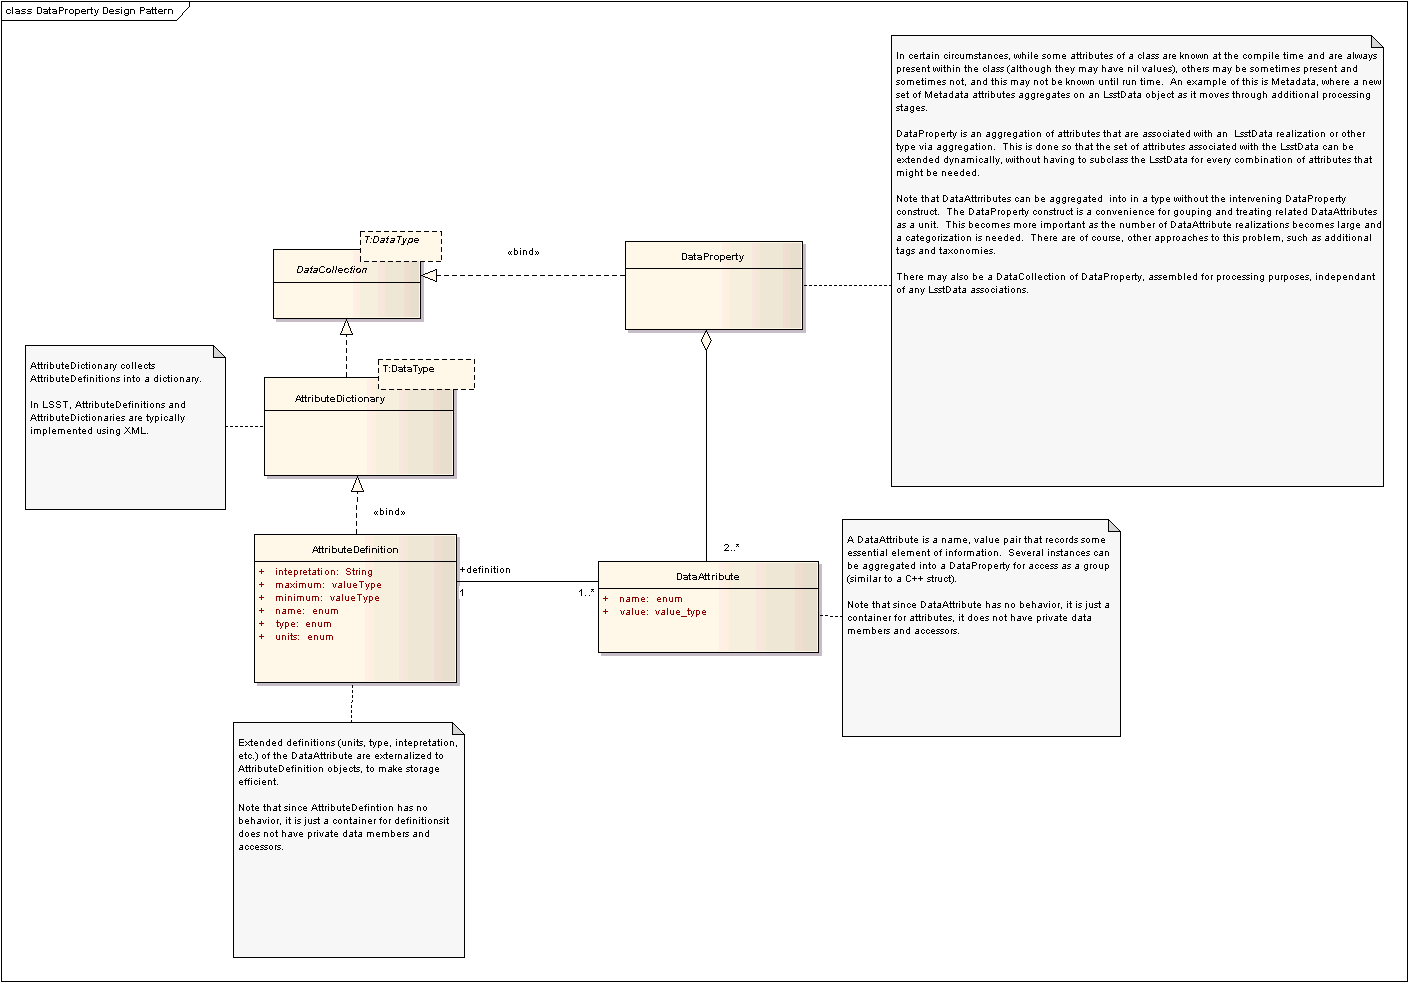
\includegraphics[width=\textwidth]{figures/DataPropertyDesign.png}
\caption{\code{DataProperty} Design Pattern}
\label{dataproperty-design}
\end{figure}


\paragraph{Issues and Lessons Learned}

The biggest issue with DC2's version of \code{DataProperty} is its data model,
which conforms best to FITS headers in allowing duplicate keys and being
order-sensitive.  Neither of these capabilities is characteristic of
the familiar key/value dictionary 
used by \code{std::map}, \code{std::hash\_map}, Java and Python
dictionaries, and the LSST \code{Policy} class (\Sec{Policy}). 
Ordered lists with duplicate keys can still be represented 
in a dictionary by using a single key
having an ordered list of values, however, and we will investigate reconciling the
data models of \code{DataProperty} and \code{Policy} in DC3.

Another issue that arose with \code{DataProperty} stemmed from its
implementation in terms of \code{boost::any}.  While this allowed any
C++ object to be inserted as a value --- a highly desirable feature --- it
meant that the recipient of a \code{DataProperty} needed to know the type of
value associated with each key at compile time before extracting that
value.  Even having execution-time metadata (e.g. from a \code{Definition}
class) describing the value type
associated with each key would not resolve this problem, as a type
switch would still be necessary.  While having such type information at
compile time (or code writing time) allows C++ to select the appropriate
value-extracting method, such code is particularly unnatural in Python,
where types are assumed to be dynamic.  In addition, explicit
construction functions for \code{DataProperties} had to be defined for Python
since some C++ types, such as \code{float} or \code{int64\_t}, are
inaccessible via implicit type matching in SWIG.  Adding utility
functions to extract integral types (regardless of size), real types, or
string types may help.

The initial \code{DataProperty} design had no easy way to combine two \code{DataProperty}
nodes.  We added an \code{addChildren()} method to allow all of the
children of one node to be added to another, replacing any of the same
name if already present.

\code{DataProperty} provides a powerful generic mechanism for sharing and
transmitting data, potentially finding uses even for communicating data
between functions in C++ or Python.  Programmers will need to be careful
to use this capability only when required, however, as passing function
arguments as a \code{DataProperty} instead of as explicit arguments may reduce
the type-safety, documentability, and debuggability of the code.

\subsubsection{Exception Classes}

An \code{ExceptionStack} class was defined to act as the main LSST exception
type.  Implementing this as a stack allows exception handlers to rethrow
exceptions without losing any underlying information.  All LSST
exceptions are subclasses of \code{ExceptionStack}.

Each exception (or level of the exception stack) can also contain a
\code{DataProperty} so that machine-interpretable key/value pairs can be
attached to the exception.  These key/value pairs are in addition to
the exception type and a human-readable exception message.

In DC2, exceptions were sometimes caught by calling code based on their
type information alone; if not, they propagated to the pipeline
framework, which handled them in an intelligent but generic,
type-independent and data-independent, fashion.  In DC3 and subsequent
Data Challenges, application-level exception handling is expected to
become more prevalent, making use of the stack and attached data
functionality described above.


\subsubsection{Trace and Logging Classes}

\paragraph{Description and Usage}

Two similar facilities were developed for emitting messages for
display that indicate what is happening in the code as it executes.
The Trace facility was developed first to serve the immediate
needs of the development phase as a debugging tool.  Later, a more
sophisticated logging facility was developed to support use cases
beyond simple debugging.  Building on the Trace design (as well as
some of the same underlying code), the logging system allows messages
to be automatically timestamped and collected from the many parallel
processes in an effective way.

The Trace facility is made up primarily of a \code{Trace} class
and a \code{TTrace} template that enable developers to produce debugging 
messages; these messages may be left in the source code
and selectively enabled by the user.  Both classes associate the
messages with a component name, which is defined hierarchically, and a
verbosity level.  The class allows the maximum verbosity level for each
component to be specified at run time, with inheritance through the
hierarchical component tree.  The template allows a maximum verbosity
level for a given source file to be specified at compile time, with no
code generated if a given message's level exceeds the compiled-in
maximum (it is also possible to compile out all Trace messages).

Trace messages may be written to any output stream, with the default
being standard error.  Since these messages are intended for debugging
purposes, there are no special provisions made for collecting them into
a central location.  

The Logging facility builds on the capabilities of Trace
in that it also supports the hierarchical component names and the
ability to tune the verbosity on a per component basis.  However, it
adds:
\begin{itemize}
\item  The ability to tag messages with arbitrary data properties;
\item  Automatic tagging of messages with standard properties,
  including a time-stamp and the node where the message originates;
\item  A convention for assigning verbosity levels to logical levels
  of severity (e.g. \code{Debug}, \code{Warn}, \code{Failure}, etc.);
\item  The ability to send messages to multiple streams
  simultaneously (with each destination having different verbosity
  controls);
\item  Pluggable message formats that can be configured on a 
  per-destination basis; and
\item  A mechanism for collecting messages from all of the nodes being
  used in an application and collating them into a browseable collection. 
\end{itemize}

The default behavior of the logging system depends on whether its
functions are called within the context of a running pipeline.
Outside of a pipeline, logging messages are simply printed to the
screen.  Inside a pipeline, the messages are converted into events and
published into the event system (\Sec{sMw-ev}).  These logging
events get sent to a separate machine where the messages and their
associated data properties are recorded into a database.  

Because all messages are timestamped, it is possible (with the aid of
the logging database) to measure the time it takes to execute a section
of code by taking the difference in the timestamps for messages
recorded at the start and end of the section.  Consequently, the
logging database is the basis of the timing analysis presented in
\Sec{sRes-time}.  

\paragraph{Issues and Lessons Learned}

As a convenience, the \code{Trace} class provided extra support
for formatting messages using \code{boost::format}.  We soon found,
however, that use of \code{boost::format} in this way would end up
formatting messages even when the messages were not getting printed
due to the verbosity setting; thus the \code{Trace} calls imposed a
significant run-time overhead.  We corrected this by providing an
interface that wraps the standard C function \code{vsnprintf} so
that the formatting of the message is done only if the message is to
be printed.  The Logging facility is susceptible to the same
problem; however, it does provide some usage patterns that prevent the
formatting overhead problem.  It does not yet support the
\code{vsnprintf} interface that is now in \code{Trace}, but it would
certainly benefit from it.  

Because the Logging facility was delivered much later than the
Trace facility, the use of the latter is more ubiquitous in our
code, particularly in the application code.  Many of those application
messages \textit{should} have been sent through the logging facility, had
it been availble, so that they could be captured, recorded, and made
use of as part of the production run timing analysis
(\Sec{sRes-time}).   

The Trace and Logging facilities intentionally share
functionality; the existence of two separate facilities is an artifact
of the development history.  In DC3, we plan to merge these into a
single logging facility that can serve both the debugging needs and
the need to record the runtime status.  



\subsubsection{SupportFactory}

The \code{SupportFactory} class was intended to be used to decorate and
configure LSST-specific data objects with appropriate auxiliary objects
to handle system-level tasks such as security or persistence.  In DC2,
this level of control was not yet necessary, so the \code{Security},
\code{Provenance}, and \code{ReleaseProcess} classes in \Fig{lsstdata-design}
were not implemented, and objects contained their own internal \code{Policy}
instances rather than using an externally-provided instance.

\begin{figure}[htbp]
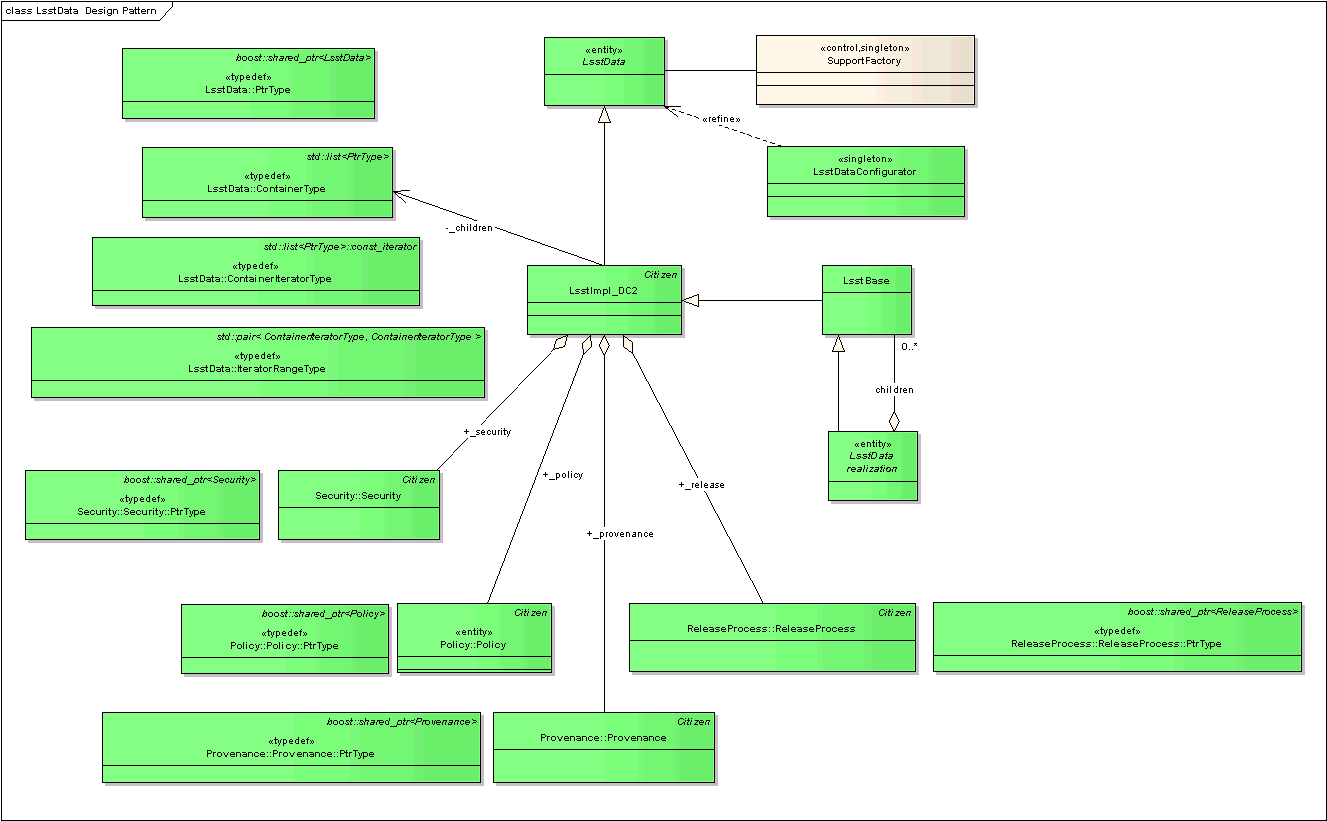
\includegraphics[width=\textwidth]{figures/LsstDataDesign.png}
\caption{\code{SupportFactory}/\code{LsstData}/\code{LsstBase} Design Pattern}
\label{lsstdata-design}
\end{figure}

Ironically, the only DC2 class for which \code{SupportFactory} was generally
used was \code{DataProperty}, somewhat contradicting the goal of having the
latter be a lightweight metadata object.  Heavier-weight classes such as
\code{Image}, \code{WCS}, or \code{Exposure} did not have their instances created using the
\code{SupportFactory} in DC2, even though they did derive from \code{LsstBase}.

In DC3, \code{SupportFactory} will not be used to create \code{DataProperty}
instances.  Its use with other classes may be introduced or mandated,
particularly as we develop functionality for its associated classes
like \code{Provenance} or \code{ReleaseProcess}.

\subsubsection{Policy Class}
\label{Policy}

\paragraph{Description and Usage}

\code{Policy} is a general-purpose class storing hierarchical key/value pairs.
It is intended for read-only data used to configure application
algorithms and pipeline components.  It was initially designed to
support up to three text-based file formats to allow both hand-editing
and machine authoring of configurations: JSON, XML, and an LSST-specific
format called the Policy Authoring Format (PAF).  In the end, JSON
authoring proved to be less popular than PAF, and it requires a
third-party package, so it will be dropped in DC3.  XML support was not
implemented in DC2, but it may become valuable as more complex uses of
\code{Policy}s are developed.

While \code{Policy}s are generally immutable, they do contain a full set of
creation and modification methods.  These are useful for testing, but
there were rare occasions in DC2 where they were used to modify read-in
\code{Policy}s (e.g. substituting for variables in patterns).  These
non-standard uses will be eliminated in the future.

Some additional \code{Policy} capabilities were not fully used in DC2.  The
ability to validate \code{Policy}s based on a dictionary of keys, types, and
values was implemented and many dictionaries were written, but
validation was not required in the final pipelines.  (Compare the
Definition and Dictionary design for the \code{DataProperty} class in
\Sec{DataProperty} above.)  The ability to include \code{Policy} files within
other \code{Policy} files also went unused.


\paragraph{Issues and Lessons Learned}

The underlying model and key/value pair implementation should be shared
with the \code{DataProperty} class, which is otherwise very similar.
\code{Policy} is
a heavier-weight class, as it also incorporates dictionaries and other
features, but the basic key/value operations should be consistent with
\code{DataProperty}.  At the same time, the supported types should be made
consistent, including support for \code{int64\_t} and \code{float}.  All
value types should be accessible from Python, with explicit construction
functions if required.

A request was made to be able to load default \code{Policies} for a pipeline
from a particular directory, overriding values in those \code{Policies} with
new ones from a different \code{Policy} file.

Another request was made to be able to use values set at a higher
level in the \code{Policy} hierarchy as the values of keys at a lower level.
This capability was designed but not implemented in DC2.

Finally, there was a request to be able to parameterize \code{Policy} values
using rules that could test conditions, presumably involving other
values or perhaps even pipeline context information.  The implications
for provenance will need to be explored.

\subsubsection{Persistence Class}
\label{persistence}

\paragraph{Description}

The persistence framework is a set of classes designed to support moving
data to and from persistent storage.  (For simplicity, we will often
refer to persistence instead of both persistence and retrieval.)  This
framework is intended to allow run-time configuration of the destination
of the persistence operation by means of \code{Policy}, to have minimal impact
on the design and implementation of the application class being
persisted, and to support high-performance implementations of
persistence in view of the large amounts of data that the LSST pipelines
will need to create and retrieve.

Persistence is mediated through a \code{Persistence} object that controls the
operation.  \code{Storage} objects provide the interface to the underlying
storage mechanism, while \code{Formatters} control the transformation from
the internal, in-memory format to the external storage format.  The use
of these classes is shown in \Fig{persistence-use}; each class is
described in more detail below.

\begin{figure}[htbp]
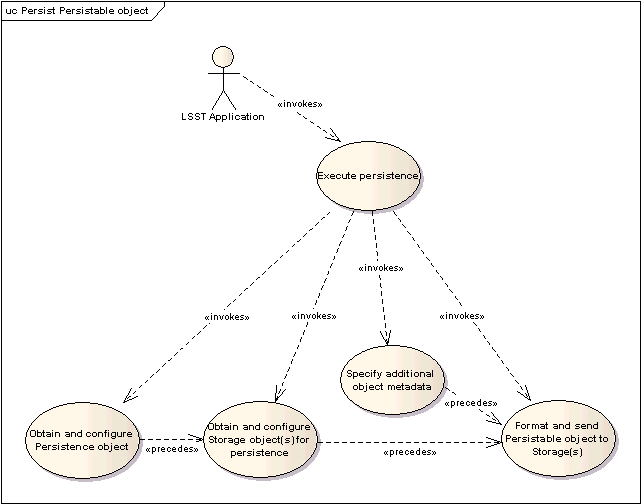
\includegraphics[width=\textwidth]{figures/PersistObject.png}
\caption{Use case for persisting an object}
\label{persistence-use}
\end{figure}

Later during DC2 development, generic input and output pipeline stages
were added to the C++ class framework in order to insulate application
stages from the details of how the data they operate on is retrieved or
persisted.  This allows the application stages to be reusable in more
contexts.

\paragraph{Major Classes}

\Fig{persistence-design} illustrates the design of the major classes in
the persistence framework.

\begin{figure}[htbp]
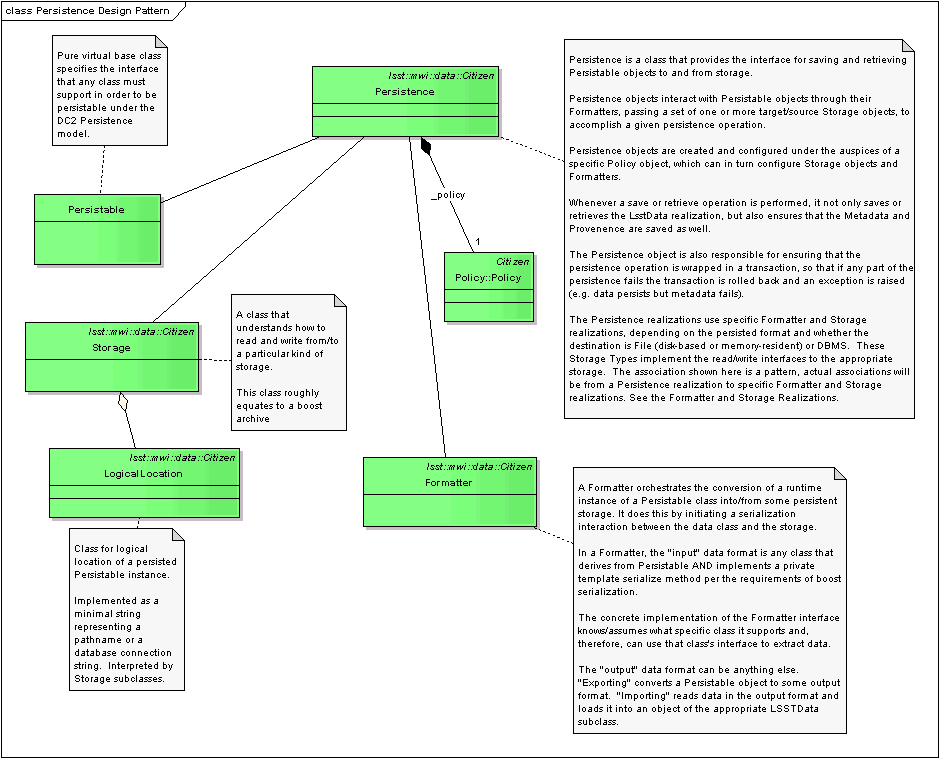
\includegraphics[width=\textwidth]{figures/PersistenceDesign.png}
\caption{Persistence design pattern}
\label{persistence-design}
\end{figure}

\subparagraph{LogicalLocation}
This class encapsulates a URL-like string that provides location
information.

\subparagraph{Storage}
This abstract base class is subclassed for each supported type of
persistent storage (see next section).  Each subclass manages all
interactions with its type of storage and provides methods used by the
\code{Formatter} classes below.  It can accept a \code{Policy} for configuration and
control.

\subparagraph{Formatter}
This abstract base class is subclassed for each persistable application
class.  Each subclass translates the private member variables of its
application class into the appropriate form for persistent storage (or
vice versa).  The subclass must contain code for each type of \code{Storage}
that may be used with the application class.  A \code{DataProperty} of pipeline
information (known as AdditionalData) is passed to the subclass to allow
selection of particular database rows or tables.  The subclass can
accept a \code{Policy} for configuration and control.

\subparagraph{Persistable}
Each persistable application class must inherit from this base class.
It provides the connection with the appropriate \code{Formatter} subclass and
also provides a method used to enable Boost serialization.

\subparagraph{Persistence}
This class manages persistence and retrieval operations.  It provides
access to the factory for \code{Storage} subclasses and selects \code{Formatter}
subclasses based on the type of \code{Persistable}.  It is intended to manage
high-level transactions to ensure the persistence operation completes or
is rolled back, although this functionality was not implemented for DC2.
It, too, can accept a \code{Policy} for configuration and control.

\paragraph{Storage Classes}
\label{Storages}

\subparagraph{DbStorage, DbTsvStorage}
These \code{Storage} subclasses manage the persistence of data to database
tables.  \code{DbTsvStorage} optimizes the persistence of large quantities of
data by writing a temporary tab-separated-value file that is then
bulk-loaded into the database.  These \code{Storages} fully isolate the rest of
the LSST software from the details of database interaction,
encapsulating connections, sessions, table management, value binding,
SQL query creation, prepared statement management, and cursor
operations.  In DC2, they were implemented on top of the CORAL
relational database portability layer from CERN, so they could be
switched from an underlying MySQL database to an Oracle database at
will.  This functionality was found to be unneeded in the short term,
and its cost in terms of the additional package that had to be supported
was relatively high, so in DC3 we will investigate reimplementing these
subclasses directly in terms of the MySQL API.

\subparagraph{FitsStorage}
This simple \code{Storage} manages the pathname needed to persist data to FITS
files in a shared filesystem.

\subparagraph{BoostStorage}
This \code{Storage} manages the persistence of data to text archive files using
the Boost serialization framework.  (Note that some data persisted to
these files may be in binary form for efficiency, despite the
description as ``text archives''.) This \code{Storage} was not used except for
testing.  It will eventually be used for checkpointing the state of
pipelines or stages.

\subparagraph{XmlStorage}
This \code{Storage} is intended to manage the persistence of data to XML files.
This \code{Storage} was not used in DC2.  Its current implementation is in
terms of Boost serialization, which results in a particular form for the
XML file.  If this \code{Storage} is to be used in the future, it may require a
rewrite to handle more general XML structures.

\paragraph{Formatters}

\subparagraph{\code{DataProperty}}
\code{DataProperty} persistence to database storage is used to maintain DC2
provenance information.

\subparagraph{Application framework classes}

While \code{Formatter} subclasses were written for \code{Image},
\code{Mask}, and other application framework classes, the primary one
used in DC2 was \code{Exposure}.  Input and output of \code{Exposure}s
from and to FITS files was supported.  In addition, persistence of
\code{Exposure} metadata, including the WCS, to a database was also
supported.

\subparagraph{Association Pipeline inputs and results}
The vectors of difference image sources (\code{DIASource}s) and moving object
predictions (\code{MopsPred}s) generated by the image processing pipeline and
nightly moving object pipeline, respectively, had \code{Formatter} subclasses
to specify their persistence to database tables (\code{DbTsvStorage}).  The
results of the association pipeline, including vectors of match pairs and
identifier pairs, were also persisted to database tables using \code{Formatter}
subclasses.

\subparagraph{Policy}
\code{Policy} did not use the persistence framework for its text-file retrieval
operations.  Since persistence is configurable by \code{Policy}, doing so would
create a circular dependency.

\paragraph{I/O Stage Classes}

Two pipeline stage classes were added to the distributed processing framework
to support generic input and output of data.  These stages were used in
DC2 to manage all persistence and retrieval of data, with the sole
exception of lookups in the database, for example to obtain filter name
to identifier mappings or moving object orbit parameters.

A sample \code{InputStage} policy looks like this:
\begin{verbatim}
AdditionalData: "exposureId=triggerVisitEvent.exposureId"
InputItems: {
    ScienceExposure: {
        Type: "ExposureF"
        PythonType: "lsst.fw.Core.fwLib.ExposureF"
        StoragePolicy: {
            Storage: "FitsStorage"
            Location: "/lsst/DC2root/%{runId}/ipd/input/%{exposureId}/
                       %{ccdId}/%{exposureId}p_%{ccdId}"
        }
    }
}
\end{verbatim}

The AdditionalData specification allows values from events or
other items on the input clipboard to be made available to the
persistence framework through a \code{DataProperty}.

The InputItems specification gives the item or items to be
retrieved, in this case a ScienceExposure.  Its type information is
provided and the type of storage and location from which to retrieve it
is specified.  The location pathname has substitutions indicated using
``\%\{\}".  Some of these substituted values (e.g. \code{runId}
and \code{ccdId}) are determined by the \code{InputStage} itself based on the
pipeline context; others (e.g. \code{exposureId}) are copied from
clipboard items.  This flexible templating facility allowed any desired
filesystem layout to be easily supported.

A sample \code{OutputStage} policy looks like this:
\begin{verbatim}
AdditionalData: "exposureId=triggerVisitEvent.exposureId"
OutputItems: {
    ScienceExposure: {
        Required: true
        StoragePolicy: {
            Storage: "FitsStorage"
            Location: "/lsst/DC2root/%{runId}/ipd/output/%{exposureId}/
                       %{ccdId}/%{exposureId}p_%{ccdId}"
        }
        StoragePolicy: {
            Storage: "DbStorage"
            Location: "mysql://lsst10.ncsa.uiuc.edu:3306/%{runId}"
        }
    }
}

Persistence: {
    Formatter: {
        ExposureF: {
            ScienceExposure: {
                TableName: "Raw_CCD_Exposure"
            }
        }
    }
}
\end{verbatim}

Here the Required specification is used to indicate that
persistence is mandatory and that the ScienceExposure must be present on
the clipboard.

Two StoragePolicy specifications are used for the single
ScienceExposure; it is persisted first to \code{FitsStorage} and then its
metadata (including the pathname used for the FITS file) is persisted to
\code{DbStorage}.

Finally, the \code{Formatter} subclass for the \code{ExposureF}
application framework class (an instantiation of the general
\code{Exposure} template) is configured to place this ScienceExposure's
metadata into the \code{Raw\_CCD\_Exposure} table in the database.

\paragraph{Performance}

The persistence framework achieved its goal of enabling flexible input
and output of application objects.  Over the course of DC2, the layout
of the input and output files changed several times, but modifications
were limited to the \code{Policy} configurations of the appropriate
\code{InputStage}s or \code{OutputStage}s.  \code{Exposure} persistence
with metadata in the database and pixels in FITS files was demonstrated.
Inter-pipeline communication via the database for difference image
sources and moving object predictions was also demonstrated.

I/O speed was not a limiting bottleneck in the DC2 pipelines, although
this type of performance will need to be monitored carefully in the
future.  Representative times for I/O operations are given in
\Table{tPersist}.

\begin{table}[htb]
\begin{center}
\caption{Timings of I/O operations using the persistence framework}
\label{tPersist}
\vspace{\baselineskip}
\begin{tabular}{| p{0.75\textwidth} | r |}
\hline
Read one slice's 10.3 MB \code{Exposure} and 10.3 MB template
\code{Exposure} from FITS files on NFS filesystem & 9.0 sec \\ \hline
Write one slice's 10.3 MB \code{Exposure} to FITS file on NFS filesystem
and metadata to database & 6.5 sec \\ \hline
Write one slice's 10.3 MB difference \code{Exposure} to FITS file
on NFS filesystem & 6.4 sec \\ \hline
Write one slice's \code{DIASource}s to database \newline
(average number of \code{DIASource}s = 36) & 0.05 sec \\ \hline
Read all \code{DIASource}s from database \newline
(average number of \code{DIASource}s = 1321) & 0.16 sec \\ \hline
Write \code{DIASource} matches to database \newline
(average number of match pairs = 1082) & 0.03 sec \\ \hline
Write new \code{Object} identifier pairs to database \newline
(average number of pairs = 537) & 0.02 sec \\
\hline
\end{tabular}
\end{center}
\end{table}

Note that DC2 was limited to a single-host NFS filesystem for image
storage.  As a result, while the per-slice I/O bandwidths achieved were
only on the order of 1.6--2.3 MB/sec, the overall I/O bandwidth to the
shared filesystem was a much more reasonable 57--83 MB/sec, especially
given the contention involved with 36 simultaneous I/O operations.

In the future, we expect to use an image store that has much larger
aggregate bandwidth and lower contention.  This might be implemented,
for example, by providing SAN connections to each compute node or by
using a Lustre parallel filesystem.  The result would be significantly
decreased image read and write times and increased scalability.

\paragraph{Issues and Lessons Learned}

A common persistence use case occurring during testing and manual
debugging is to persist an application object to a single type of
storage.  Performing this operation currently requires several steps in
Python.  A convenience function to simplify this use case into a single
step will be provided.

Information used to specify the location of persisted objects is
provided in various places, including the AdditionalData
\code{DataProperty}, the Location in the StoragePolicy specification of
the \code{InputStage} or \code{OutputStage}, and in some cases items in
the \code{Formatter} \code{Policy}.  These should be merged
into a single \code{DataProperty}, perhaps as part of the
\code{LogicalLocation}.

The facility for substituting values into the location strings is
valuable, powerful, and flexible, but it adds yet another syntax to
learn.  The standard Python syntax and formatting mechanisms will be
used to simplify usage.

% Subsection 3.1: fw -*- latex -*-

\subsection{Framework}
\label{FW}

For DC2, we split the LSST framework into two
parts, MWI (Middleware Interface; \Sec{MWI}) and FW.
Each lies in its own namespace (\code{lsst::mwi} and \code{lsst::fw}).

\subsubsection{C++ Classes}

FW contains the framework classes related to processing astronomical images.
The fundamental objects are:
\begin{itemize}
\item Images and Masks
  \begin{itemize}
  \item \code{Image}:
    A 2-dimensional image.
  \item \code{Mask}:
    A set of 2-dimensional bitmasks.
  \item \code{MaskedImage}:
    A container of two \code{Image}s (the data and its variance) and a \code{Mask}.
  \item \code{WCS}:
    A World Coordinate System class.
  \item \code{Exposure}:
    A \code{MaskedImage} and its \code{WCS}.
  \end{itemize}

  \item Convolution Kernels
    \begin{itemize}
      \item Kernels: \code{AnalyticKernel}, \code{FixedKernel}, \code{Kernel}, \code{LinearCombinationKernel}.
      \item Kernel's spatial variability: \code{Chebyshev1Function1}, \code{GaussianFunction1}, \code{Lanczos\-Function1},
	\code{PolynomialFunction1} (and their 2-dimensional analogs).
      \item Free functions to convolve \code{MaskedImage}s with Kernels.
    \end{itemize}

  \item Miscellaneous:
    \begin{itemize}
    \item \code{MaskedImageFormatter}:
      Using \code{boost::persistence}.
    \item\code{DiskImageResourceFITS}:
      Saving image and mask data to FITS files.
    \item \code{MovingObjectPrediction}:
      A prediction of the current position of an object.
    \item \code{DiaSource}:
      The properties of a source detected in a difference image.
    \item \code{Filter}:
      A photometric filter (e.g.~\textit{g}).
    \end{itemize}
\end{itemize}

All of these classes were implemented for DC2, and make use of
the support classes defined in mwi (e.g.~\code{mwi::data::LsstBase},
\code{mwi::utils::Trace}).  They are documented using doxygen (\Sec{build_docs}),
although the level of the documentation is patchy; in particular,
high-level documentation (motivation and examples) tends to be 
missing. The documentation will be expanded in DC3.

\paragraph{Images and Masks}

\subparagraph{Image and Mask}
The classes that contain pixels (\code{Image}, \code{Mask},
\code{MaskedImage}, and \code{Exposure}) use JPL's VisionWorkbench
(VW) to provide the fundamental pixel access; specifically
\code{Image} and \code{Mask} contain a \code{vw::ImageView}.

We have adopted two idioms to access pixels in DC2: registering
a functor (derived from \code{fw::PixelProcessingFunc}) that should be applied
to each pixel in the image, or explicitly iterating over the pixels.

The functor approach is clean and object-oriented, but not very well
suited to algorithms that process sets of pixels (e.g.~searching an
image for connected pixels over threshold).  This approach was used e.g.~in
measuring the centroid of a detected source.

Explicit pixel access in VW uses an iterator rather than a pointer to
access the pixels, although the VW header files state that the
STL-compliant iterator (\code{vw::PixelIterator}) is slow, and should
not be used in time-critical applications.  An alternative,
(\code{vw::ImageView::pixel\_accessor}) may be used but is not a full
STL iterator; we opted to use accessors for DC2.  These proved not to
be rich enough to easily express common operations (e.g.~returning the
value of the pixel just to the right of the accessor), but minor
enhancements to the API would probably resolve these difficulties.

The implementation of subsets of images is not complete; for example
there is no \code{Image} API to get a sub-\code{Image} that shares
pixels with the full \code{Image}.  The code that uses subimages
does not uniformly and consistently allow for coordinate offsets,
although this is likely to be a fruitful source of confusion in
future data challenges.  How to do this consistently and transparently
is not obvious.

\subparagraph{Mask}
LSST's bitplane class uses a dictionary to associate named planes
(e.g.~\code{SATUR}) with bits (e.g.~\code{0x10}); the planes themselves
are implemented as bitmasks within \code{vw::ImageView} as described above.

This representation was chosen to allow us maximum flexibility --- in
particular to allow modules to add planes as needed, and to import
external masks (e.g.~CFHT bad-pixel masks).  During DC2 we realised
that this flexibility came at a cost;  in order to apply operators
to \code{Mask}s the bitplane dictionaries must first be reconciled,
and this expensive step will be needed whenever different modules
add the same planes in varying orders.

For DC3 we intend to preserve the flexibility of named, extensible
bitplanes, but make the dictionary a class variable rather than an instance
variable (\ticket{322});  we expect this change to remove the
need to reconcile \code{Mask}s.

\subparagraph{MaskedImage}
We represent images with associated masks and variances using \code{MaskedImage},
with pixel accessors similar (but not identical) to \code{vw::ImageView::pixel\_accessor}.
These have proved viable, but not especially flexible;  for example, there is
no clean way to read a neighboring pixel value without also moving the mask and
variance iterators.

\subparagraph{\code{WCS}}
LSST's world coordinate system class is currently implemented using Mark Calabretta's 
\code{wcslib}\footnote{http://www.atnf.csiro.au/people/mcalabre/WCS}
which represents the WCS in terms of FITS keywords, stored internally to \code{WCS}
using \code{DataProperty} (\Sec{DataProperty}).  This has proved satisfactory
for DC2, although the CFHT images caused problems with \code{wcslib}'s \code{wcsfix}
function (\ticket{184}) and \code{wcslib} fails to read some apparently legal
FITS headers (\ticket{259}).

\paragraph{Convolution Kernels}

\subparagraph{Kernel}
\code{fw} supports a number of types of kernel derived from a class \code{Kernel}:
\code{AnalyticKernel},
\code{FixedKernel}, \code{LinearCombinationKernel}.  These can be thought
of as small images, and are used to represent difference kernels (\Sec{ImageSubtraction}), and
will in the future probably also be used to represent point spread functions,
PSFs.

An \code{AnalyticKernel} is defined by a function that can be used to evaluate
any pixel within the kernel; a \code{FixedKernel} has the pixel values provided
explicitly, and a \code{LinearCombinationKernel} is a linear combination of
other kernels (e.g.~a set of Gauss-Hermite functions).  In general kernels
are spatially varying, and \code{fw} provides a number of classes to express
this: \code{Chebyshev1Function1}, \code{GaussianFunction1}, \code{LanczosFunction1},
\code{PolynomialFunction1} (and their 2-dimensional analogs).

Once a (possibly spatially varying) Kernel is defined, it may be
applied to a \code{MaskedImage} to generate the convolution of the
image with the specified kernel, taking proper account of the mask and
variance.  In the future we expect to also support convolving single
\code{Image}s.

There are some concerns with the speed of convolution in DC2.  In the
context of difference imaging, this has been partially resolved by
adding a new kernel type, \code{DeltaFunctionKernel}, and providing
a specialisation of the convolution code to exploit the special structure
of a Kernel with only one non-zero pixel; this specialization has
not been deployed in DC2.

\paragraph{Miscellaneous}

\subparagraph{Persistence}
See the discussion in \Sec{persistence}.  The \code{fw} package
provides support for persistence in terms of classes that
implement \code{boost::persistence} for e.g.~\code{MaskedImage},
and that are able to save image and mask data to FITS files.

\subparagraph{MovingObjectPrediction}
This is a prediction of the current position of an object, including
errors.

\subparagraph{DiaSource}
This holds the properties of a source detected in a difference image.  The
class itself contains a large number of parameters as
expected by the database, but only a few are actually measured
for DC2;  even for these, only place-holder algorithms are
employed.

\subparagraph{Filter}
This identifies a photometric filter (e.g.~\textit{g}).

% \subsubsection{Python}  Moved to build.tex and generalized for all
%  of DC2


%  \subsubsection{Testing}  Moved to build.tex and generalized for all
%  of DC2

\subsubsection{Timings}
\label{fwTiming}

The DC2 implementations of critical functions are still slower than we
need.  A preliminary investigation focussed on the convolution
operations, hoping that lessons learned will apply wherever we look at
pixels.  We are analyzing the code at various levels, including at the
assembler level to understand the efficiency of our most
compute-intensive loops.  It is clear to us that there is work to be
done.  In particular, we find an over-abundance of register loads
(this might be better on more modern processors), and pointer updates
are not simple offsets by compile-time constants (e.g.~4).  It seems
likely that a few well chosen changes to the lowest level accessors
could significantly improve performance while remaining transparent to
the user-level code.


% Subsection 3.2: mwi

\subsection{Database}
\label{database}

DC2 used as the underlying DBMS the MySQL Community Edition version 5.0.45.
A single database server was used, running on a dedicated commodity
machine (lsst10) with dedicated SAN-attached disk storage.
Each DC2 run created and used a separate dedicated database. At the end of DC2 
we had over 200 databases, occupying a total of 126 GB of disk space.

\subsubsection{Schema}

The DC2 database schema consisted of 23 tables. These tables covered
all DC2 products requiring the database, including objects, 
difference sources, moving objects, predicted positions of moving objects 
and their orbits, exposure metadata, and some internal association-related 
tables. In practice this is a small subset of the entire LSST schema, 
which currently consists of over 100 tables. The full LSST schema, 
in addition to products used in DC2, includes a draft schema for provenance 
and calibration related tables.

The schema of the tables used in DC2 was very similar to the schema of the
corresponding tables in the LSST schema. Even though in DC2 we did not 
need all the columns from tables like Object or DIASource, we kept them
to maintain realistic row sizes.
The DC2 specific changes applied to the schema were related to specifics
of the CFHT input data. These changes include adding a few columns to 
the Object table and keeping exposure metadata at a different level ---
in DC2 we kept exposure metadata at the CCD level, while in production we 
expect to manage detailed exposure metadata at the level of individual 
amplifiers. 

\subsubsection{Usage}

The main role of the database was to act as a persistent store and
allow efficient querying of the catalogs and metadata.
An additional role of the DC2 database was to act 
as a communication channel between the pipelines --- in particular,
between the IPD and association pipelines and between the MOPS
and association pipelines.

In the former case the IPD pipeline wrote newly detected 
difference sources to the database, and the association pipeline read them.
The communication was done through a dedicated in-memory table.
In the latter case MOPS wrote predicted
positions of moving objects to the database, again for reading by the
association pipeline.

\subsubsection{Direct Ingest Without Catalog Ingest Service}

One of the main differences from our database usage
in DC1 was the removal of the Catalog Ingest Service (CIS).
In DC1 each processing slice dumped data into a well known
location, and CIS ``pulled'' the data and inserted it
into the database. Such an approach allowed us to avoid multiple concurrent
inserts into the same set of tables --- CIS concatenated all
the smaller inserts into a single bigger one. In DC2 we decided to test a 
different approach: we removed CIS, and allowed individual slices 
to ``push'' data directly into the database (via the Persistence
framework). 

To ingest data efficiently we used tab separated value (TSV) files --- 
the most efficient technique to insert multiple rows into a MySQL 
table. This technique was also used by CIS in DC1. Each slice used 
its own TSV file. Since all tables (except a few MOPS-related ones) 
were of MyISAM type, table-level locking was used, which is 
the worst-case scenario when performing concurrent inserts. 
Inserts were done \textit{ad hoc}, without any attempt to synchronize or 
de-synchronize them. In practice, due to enforced synchronization 
on stage boundaries, all slices wrote to the database at almost the same time. 
Again, this is the worst-case scenario. In DC2 we had 36 slices, 
and each slice wrote 36 rows on average. On average, it took 
a very reasonable 0.05~sec per slice to complete the ingest.

In production, we are expecting to have about 3000 slices --- one per amplifier.
Each slice will produce a few dozen new difference sources.
Should lock collisions be a problem due to the larger number of
concurrent inserts, we could switch to a MySQL table type with row-level 
locking or go back to the CIS-like approach and combine multiple 
ingests into a single bigger one.

\subsubsection{Issues and Lessons Learned}

Based on standalone tests we ran in 2007 prior to the DC2
final runs, we determined that in order to meet the 10~second
real time requirement for the Association Pipeline, we needed to
move some of the processing out of the database itself into custom-written
code, and maintain a specialized copy of some data used by AP 
in a custom file format, rather than keep it in the database. 
Such an approach allowed us to tailor the match algorithm specifically 
to our needs, and take advantage of data locality and partitioning. 
More details about this approach, including the partitioning scheme, can 
be found in \Sec{association} of this report.

It might be possible in future versions of MySQL to teach the
query optimizer to deliver a query plan similar to our custom 
algorithm.  Today, however, such a task is very difficult if not impossible. 
This is likely true for most, if not all, DBMS products available 
today. We will periodically re-evaluate the custom versus in-database 
approach, and will work with DBMS vendors on extending their 
optimizers to better meet our needs.

In all the places where MySQL was used, performance was not 
an issue. This is true for both ingesting and querying the data.
Essentially the database overhead was negligible. 

% Subsection 3.3: harness

\subsection{DPS: Distributed Processing Services}
\label{DPS}\label{sMw-har}

The Pipeline Harness is encapsulated within the Distributed Processing Services (DPS) package
and uses the namespace \code{lsst::dps}.  
The distributed processing framework of the \code{dps} package provides the ability to run an application 
pipeline in parallel across numerous nodes of a cluster or supercomputer, or
across cores of a workstation, 
in transparent fashion, shielding the application codes and their developers from the details
of parallel processing.  It provides the mechanism for integrating a piece of application code 
into  a pipeline as a single stage, and provides the infrastructure for combining multiple 
application stages in sequence to form a full pipeline. It also facilitates the  triggering of 
processing within pipelines through its use of the events system of the \code{events} package
(\Sec{sMw-ev}).  
In DC2,  \code{dps}
package classes were implemented in Python and C++, and the Message Passing Interface
(MPI) was used for parallel processing and communication. 

% A wide range of the pipeline functionality within the DPS package is configureable through  policy.

\subsubsection{Pipeline and Slice}

\paragraph{Description and Usage}

The LSST baseline model calls for classes \code{Pipeline} and \code{Slice} to encapsulate the serial and parallel 
threads of pipeline processing, respectively.  For DC2, \code{Pipeline} and \code{Slice} classes were implemented
in a mixture of Python and C++.  Most of the policy configuration, stage management,  and processing workflow 
and triggering was encoded within the Python classes, while the C++ classes strictly managed 
the MPI environment.  For DC2,  MPICH2 v1.0.5\footnote{http://www.mcs.anl.gov/research/projects/mpich2}
was the message passing library utilized.  
Furthermore, serial Pipelines made use of explicit MPI2 spawn functionality to launch $N$ \code{Slice} 
workers across a collection of nodes.   The MPI communication between \code{Pipeline} and \code{Slice}s was 
collective in nature and intercommunicator-based (i.e., accomplished using MPI\_Bcast 
and MPI\_Barrier calls across the intercommunicator generated by the MPI2 spawn). 
MPI communication of complex types such as \code{DataProperty}'s between \code{Pipeline} and \code{Slice}s 
was left out of the scope of DC2, and was instead accomplished via the \code{events} system for 
this version of the harness. 

Within DC2, \code{Pipeline} and \code{Slice} were configurable through \code{Policy}, and each of the parallel threads 
read the pipeline policy file to obtain required information for setup (policy parameters are 
not communicated through MPI).  Values typically included in a pipeline policy file include the 
names of the application stages to be executed  by the pipeline, the event triggering dependencies 
of the stages, the events system broker to be used, an event topic for clean system shutdown,
and others. 

\paragraph{Issues and Lessons Learned}

There are several issues with respect to current MPI usage that are worth consideration.
The use of collective MPI communications offered a fairly clean and simple approach for DC2, 
but introduced some fault tolerance issues, as a single \code{Slice} failing could impact the full 
complement of \code{Slice}s adversely.   Some extra coding was required to keep the broader 
collection of \code{Slice}s  executing in the event that one \code{Slice} 
encountered an exception, and it  is not clear that this is the cleanest solution.
Beyond the matter of collective communication, we also need to consider whether a single \code{Pipeline}
communicating to $ N $  \code{Slice}s will scale successfully to thousands of \code{Slice}s. 
We observed the parallel pipelines of DC2 to operate in a stable fashion with a single \code{Pipeline} 
managing on  the order of $\sim40$ \code{Slice}s, but it is not known if this will scale to large numbers. 
Further stress testing of the current approach to larger scales and the investigation of more 
versatile and robust communication and \code{Slice} management are important threads of activity for
DC3 preparation. In any case, the \code{dps} Python and C++ codes provide a stable interface
such that, should we provide alternative implementations, the application codes and the
rest of the middleware will be unaffected.

\subsubsection{Stage}

\paragraph{Description and Usage}

In the LSST baseline the generic class \code{Stage} is used to wrap a single module of 
astronomical pipeline processing.  Developers write application stages by extending the 
\code{Stage} class of \code{dps} package  and implementing the \code{Stage} API. 
For DC2, this  consisted of the  methods \code{preprocess()} and \code{postprocess()} for 
serial elements to be executed within Pipelines, and the
\code{process()} method for parallel processing to be executed by Slice workers. 
This API implementation provides the code hooks by which the application code interfaces with 
the framework of the harness. The current  implementation always occurs in Python, and 
so all application stages are either written in Python or have a top layer of Python that 
invokes underlying C++ code using Python bindings generated by SWIG.  

In addition to providing the generic Stage, for DC2 the \code{dps} package also
featured  special subclasses  of \code{Stage} to provide reusable functionality pertinent  to  
multiple pipelines. These included: 
\code{EventStage}, \code{InputStage/OutputStage}, and \code{SymLinkStage}.

\paragraph{Issues and Lessons Learned}

Each of the elements of the Stage API (\code{preprocess()}, \code{process()}, and  \code{postprocess()}) 
served a needed role in enabling application Stage functionality and in facilitating the
integration of application Stages into the harness framework. The use of Python as the layer for
the final integration did not pose a hurdle to the development of the application Stages. 
The DC2 experience is overall  supportive of the  continued use of this construct for bringing 
application code  into the  pipeline  framework provided by \code{dps}. 


The idea of encapsulating generic, pluggable  functionality within modular Stages (as opposed
to encoded functionality directly into the harness)  was very useful in DC2, 
and will be further developed in future work.



\subsubsection{Clipboard and Queue}

\paragraph{Description and Usage}

The pipeline harness constructs application Stages with an InputQueue and an OutputQueue,
such that for $N_s$ total Stages there are $N_s+1$ Queues; the OutputQueue of Stage $i$ is 
identically the InputQueue of Stage $i+1$. 
Application Stages obtain parameters and data they required from a dictionary type 
structure encapsulated in the Clipboard class; an application Stage pulls the Clipboard
from its InputQueue, retrieves and adds values, and posts the Clipboard to its OutputQueue 
for the next Stage. Though the Queue may contain multiple Clipboards, in DC2 a single Clipboard was used to  carry data and information to application Stages.  

The Clipboard served to insulate application
Stages from issues of inter-pipeline communication and the middleware layer events system.
If  a given application Stage required a trigger event prior to execution, the harness framework
blocked for the arrival of the trigger event. Upon receiving the event, the \code{dps} harness places 
the payload onto the Clipboard of the serial Pipeline and all Slices under the key of the 
incoming event topic.   

In addition, an application Stage could expect to find required data
(for example, image data) on the Clipboard.  Such data would arrive on the Clipboard by 
configuring the Pipeline to begin with (or just include) an InputStage. The InputStage makes use 
of appropriate Persistence framework utilities to read data off of disk into memory and place it on the Clipboard under a  standard key for
the application Stage.   In this way application Stages could be  coded  to expect to 
find required parameters and data on the Clipboard as provided by the middleware harness.

The Clipboard mechanism also plays a role in the  current strategy for inter-pipeline communication.
 A pipeline may send an event to a separate running pipeline by executing an 
EventStage. The EventStage is configured through policy to pull \code{DataProperty}'s off of the
Clipboard under a specified key, and issue an event with these objects as payload under a 
specified event topic.   On the receiving end, the  payload is placed on the Clipboard as 
previously described.  Thus, Clipboards are effectively used to carry information from 
one application Stage to another both within and between running pipelines. 

\paragraph{Issues and Lessons Learned}

Memory management with respect to Clipboards required some care in DC2.
Across multiple visits,  a running Pipeline or Slice  could accumulate data in memory on Clipboards
if proper cleanup/garbage collection did not occur.   In DC2, all Clipboard contents were erased at the
end of the processing for each visit, and it was verified  that running pipelines had stable memory usage 
across multiple visits.  This feature also enforced that there was no dependency of the processing
of one visit on previous ones, which has important consequences for reproducibility of results
in targeted or bulk reprocessing. 

\subsubsection{Exceptions, Logging, and Other Features}

\paragraph{Description and Usage}

Exception handling by the harness framework when invoking the Stage API methods
played an important role in DC2.   
Exceptions thrown within underlying application code and not dealt with in
the lower layers were captured by the framework to prevent problems in one Slice from 
affecting the full parallel computation. If one Slice encountered a fatal exception, this fatal error
was appropriately logged (so as to be visible within the events log/portal) and the affected Slice 
was cycled through its remaining stage loop for the given visit within attempting any further 
computation, and without affecting the other Slices.

The harness also supports the capture of a shutdown event for terminating 
pipeline execution and bringing down the MPI environment cleanly.  The
topic of this event may be set in policy.  The effect of the shutdown event 
is to terminate execution at the end of the current Stage loop, even if other trigger 
visit events have been issued and data awaits processing.  An extension of this idea
will be implemented in the future, whereby a ``final data'' event (an event communicating
that  there is no more data or trigger events  forthcoming) may be issued.  In this case
the execution will terminate after all remaining  trigger visit events and their associated 
data are processed.



% - communication of values between Slices/sharing of information on Clipboards




\subsection{Pipeline Control}
\subsubsection{The Event System}\label{sMw-ev}

The event system is a set of components that can send and receive reliable, 
asynchronous messages.  Components using the event system API subscribe to a 
\textit{topic} to send and receive messages.   A message sent to a topic will be sent
to all current subscribers on that topic.    The subscriber can then decide 
what to do with that message based on its contents.   For example, in DC2, one
message sent to a topic would cause one subscriber to the start the next stage
of a pipeline,  while another subscriber to that same topic would simply 
store the entire message in a database for later analysis. 

The event system uses libraries and brokers that implement the Java Message 
Service (JMS) protocol, a widely used, robust, open source standard. There are
a number of commercial and open source distributions of JMS available.  The 
Event System API was implemented using the open source C++ messaging library 
ActiveMQ-CPP\footnote{http://activemq.apache.org}.
The Event System API is a layer above ActiveMQ-CPP; we used 
Swig to expose this API to Python. 

The Event System API hides the configuration requirements of the ActiveMQ-CPP
library, simplifying the creation of components that send and receive
messages.  To create a message transmitter, the component can make one call 
specifying the location of the message broker, and the topic to send
subsequent messages to.   A component wishing to receive messages would 
create a message receiver specifying the message broker and the topic to 
subscribe to.    Messages send on a topic by the event transmitter would then
be received by the component that created the event receiver.   Creation of
these transmitters and receivers can be done individually, or globally to 
further simplify configuration by using policy files.  There are also
interfaces to allow out of order message retrieval and message reception
timeouts.

The Logging API was used to transform logging messages into events.  These
events were sent out on a logging topic.   We used the open source messaging
platform \code{Mule}\footnote{http://mule.mulesource.org}
to create a client that received event messages from the logging
topic and sent them to a database.  Events for pipeline coordination were also
sent to a database.  These events were then later searched to identify 
problems, and to do analysis of completed runs.

\subsubsection{Launching DC2 via the Orchestration Layer}\label{sMw-orc}

In the LSST reference design, the \emph{orchestration layer} is a
component of the DMS that is responsible for preparing and configuring
a pipeline, executing it on a parallel platform, monitoring its
progress, and cleaning up the results after it has finished.  More
specifically, the preparation and execution of a pipeline would
triggered by an event containing a logical name for the pipeline to
run, along with logical identifiers for the data it is to operate on.
The logical pipeline name would be used to ``look up'' the appropriate
policy files in a policy repository.  The policy files would be
retrieved, possibly tweaked, and then deployed onto the target
platforms as necessary.  

In DC2, the orchestration layer was not a component of focus;
nevertheless, we did require the ability to setup and execute the DC2
pipelines in a consistent and automated way.  This functionality was
built into a package called \code{dc2pipe}.  Even though this
package is not intended to be an attempt to meet the general
orchestration layer requirements, it does share in some of the
concepts from the reference design.  

The pipelines are launched via a core script called \code{launchDC2.py}.
It is configured via a top-level policy file which sets some global
parameters such as the working home directory for the execution
(\code{/lsst/DC2root}), the directory representing the policy
repository, and the file containing the list of exposures to process
through the pipelines.  This policy file also sets some
pipeline-specific parameters.  Most important is the list of nodes to
run the pipeline on along with the number of processes to run on each
node.  When the \code{launchDC2.py} script is executed, the operator
passes in this top-level policy file and a name to give to that
particular execution (the \emph{run-ID}).  To prepare for the
execution, this script will: 
\begin{itemize}
\item Ensure that MPI and ssh are properly configured to execute the
execution;
\item Create the run-specific database tables to be used in the
database;  
\item Create a working home for the execution named after the run-ID 
under \code{/lsst/DC2root} for holding input data, output data, and
configuration information; and
\item Cache copies of the pipeline policy files to the working home.
\end{itemize}

Once the preparation is complete, the script executes the pipelines,
each as an MPI application on the configured head node for the
pipeline.  





% -- Section 5
\section{Application Layer}

The preceding chapter described the software infrastructure upon 
which the DC2 pipeline was created and run. Although these
components are all a necessary part of DC2 --- and will continue
to play a role through the life of the LSST project --- none of them can
accurately be described as fundamentally astronomical or
photometric in nature. Instead, they form the framework upon which 
the actual science application is constructed. We turn now to 
a description of the application layer of DC2.

% Subsection 4.1: imageSubtraction

\subsection{Image Subtraction}
\label{ImageSubtraction}\label{sApp-imsub}

The essence of Image Subtraction is to design a convolution
\code{Kernel} $K$ that  photometrically registers the
point-spread functions (PSFs) of two images.  One image is (ideally)
an essentially noiseless and defect-free template image $T$ created through
coaddition of many individual science images.  The other is the
science image $I$ obtained on a given night.  After registration,
subtraction of the template image from the science image should yield
a difference image $D$ that contains only those things that have
varied in position or brightness from the template.

Since this process involves the convolution of an image, for DC2 we
decided that we will \textit{always} build the \code{Kernel} to operate
on the template image, leaving the science pixels untouched.  The
advantages of this are two-fold: since convolution is
expected to be a smoothing process, you can afford to correlate the
pixels in the template image more than you can in the science image
since they are less noisy; and since the template is assumed to be
defect-free, we can minimize the effect that convolution spreads the
influence of bad pixels.  

The creation of $D$ is a fundamental role of LSST's nightly pipeline.
This image will feed the nightly alert stream, which will be the public face
of LSST for many scientists.  It's important we get this part of the
reductions right, which is why we began development of this stage in
DC2, with large lead time to first light.

\subsubsection{Key Framework Classes}

Image Subtraction required design and development of several key
Framework and Detection classes.  The key Framework classes developed
during the course of DC2, and how they were used, are listed below.

\begin{itemize}
\item \code{lsst::fw::Exposure} ---
   Input images from the CFHT were read into \code{Exposures}, a
   combination of a \code{MaskedImage} and its associated \code{WCS}.
   The template and science image \code{MaskedImages} were the
   fundamental objects being passed between the Image Subtraction
   stages.

\item \code{lsst::fw::Kernel} ---
   Three sets of convolution \code{Kernel}s were created in the DC2
   implementation of Image Subtraction.  They were used to match the
   PSFs of the two images in different \code{Footprint}s.  A spatial
   model was also built using the \code{Function} class below.

\item \code{lsst::fw::function::Function} ---
   This allows the user to create one or two-dimensionally spatially
   varying functions.  DC2 used \code{Functions} to represent the
   final spatially varying Image Subtraction \code{Kernel}, as well as
   a spatially varying differential background correction.

\item \code{lsst::fw::function::MinimizerFunctionBase} ---
   This internal class allows the user to fit for the coefficients of
   a \code{Function} using \code{lsst::fw::function::minimize}, \
   given a set of input constraints.  
   \code{MINUIT}\footnote{http://www.cern.ch/minuit} was used for
   the non-linear fitting backend.

\item \code{lsst::imageproc::DiffImContainer} ---
   A \code{DiffImContainer} was created for each \code{Footprint} used
   to constrain the \code{Kernel} model.  It holds pointers to the
   different versions of \code{Kernel}s that were built, summary
   statistics on the associated difference images, the background
   measurement at its position, and if the \code{Footprint} has passed
   or failed goodness-of-fit criteria.

\end{itemize}

\subsubsection{The Algorithm}

Image Subtraction is implemented using a combination of controlling
Python scripts and number-crunching C++ code.  To
create a useful reference for future designers, we will distinguish
which operations are implemented in which language.

The first stage is implemented in Python.  It reads the CFHT
template and science images from disk, and turns them into two
\code{MaskedImages}.  It also reads in the \code{Policy} file that
controls e.g.~the \code{Kernel} sizes, how large to make the
\code{Footprint}s, how faint one should go when searching for these
\code{Footprint}s, and the criteria used to reject bad
\code{Footprint}s during the \code{Kernel} creation process.

The Python code then calls the C++ routine
\code{getCollectionOfFootprintsForPsfMatching}.  This in turn calls 
the \code{Detection} code to search for significant peaks above
background in the Template image.  For reduction of commissioning
data, we will likely have to operate in this mode.  However, for
subsequent operations we should be able to query the Database for the
locations of appropriate positions.  These are returned as a list of
\code{Footprint}s.  Each \code{Footprint} is then searched for 
masked pixels in both the Template and Science images.  Any masked
pixels in the \code{Footprint} causes it to be rejected.  They are
then grown by a certain amount specified in the \code{Policy}, and
returned to the controlling Python script to have PSF-matching
\code{Kernel}s built for each one.

For each returned \code{Footprint}, a \code{DiffImContainer} is
created in Python, and the first \code{Kernel} is created.  The
C++ routine \code{computePsfMatchingKernelForPostageStamp} \
generates \code{Kernel} Model I for a given \code{Footprint}.  This
uses a delta-function set of basis functions to create the most
general \code{Kernel} possible.  The associated difference image is
examined, and the \code{Footprint} is rejected if the residuals are
too large (``too large'' having been defined in the input
\code{Policy}).  The outputs are a single \code{Kernel} and a DC
differential background correction between the template and science
image.

In Python, the \code{Kernel}s are examined as an ensemble.  In
particular, the distribution of the \code{Kernel}s sums (the
photometric rescaling, or the \code{Kernel}s ``volume'') is examined
and outliers are rejected.  These outliers might be e.g.~variable
stars.

Next the C++ function \code{computePcaKernelBasis} is called.
The inputs are the ensemble of good \code{Kernel}s.  This routine runs
a Principal Component Analysis (PCA) on the ensemble, creating an
orthonormal basis set of eigen-\code{Kernel}s from the data
themselves.  The hope is that the input \code{Kernel}s are
similar enough to justify approximating each one with a compact
set of eigen-\code{Kernel}s.  The number of eigen-\code{Kernel}s
chosen was defined in the \code{Policy}, and for DC2 was a minimum of
3, and enough to account for 95\% of the variance, up to a maximum
of 7.
%
Each input \code{Kernel} is approximated by deriving the coefficient
in front of each eigen-\code{Kernel} through their dot product, a
process that yields \code{Kernel} Model II, a PCA approximation of
each input \code{Kernel}.  The associated difference image is
examined, and the \code{Footprint} is rejected if the residuals are
too large.  If any are rejected, the PCA is re-run, until this
process converges.

Finally, the Python code calls the C++ routine
\code{computeSpatiallyVaryingPsfMatchingKernel}, which fits 
spatially varying \code{Functions} to the eigen-\code{Kernel}
coefficients (yielding \code{Kernel} Model III) as well as a spatially
varying background.  The spatial orders are specified in the input
\code{Policy}.  This allows a \code{Kernel} to be generated for, and
applied to, each pixel in the input images, allowing creation of the
difference image.  The difference image is persisted as a
\code{MaskedImage} and the \code{Kernel} and background as
\code{Functions}.

\subsubsection{Performance}
\label{ImageSubtraction-Performance}

For DC2, the \code{Kernel} Model I was very successful.  The mean
residual (normalized by the noise) across all \code{Footprint}s was
0.00, while the variance of this distribution was 1.06.  The final
variance is derived from the quadrature sum of the science image's
variance and the template image's variance (assumed to be zero for
DC2) convolved with the square of the \code{Kernel} values.  We find
that much of the extra noise came from \code{Footprint}s which should
have been masked but were not, due to e.g.~unrecognized saturated
stars.  Ideally, these \code{Footprint}s would have been skipped had
we had access to the imaging data from the start.  However,
significant pre-processing was done by the CFHT team and we were not
able to determine exactly which pixels had been saturated.
\code{Kernel} steps II and III were executed in DC2 with effectively
no sigma clipping of the input \code{Kernel}s.  This led to a success
rate of 98.7\% on the input CFHT images, with the remaining 1.3\%
having an anomalously large number of
detections per difference image.  This is commensurate with the
success rate for modern difference imaging pipelines.

The egregious failures (1.3\% of the input data) had two origins.  The
first were misregistrations of the input data, which was
out-of-scope for DC2 but will be in-scope for DC3.  These may be
recognized due to the very small ($\sim 0.0$) \code{Kernel} sums, as
the code tries to take an object in the template and match it to the
science image, which in general has no signal at that position.  The
second was a true failure of the pipeline.  These difference images had
\textit{very} strong gradients in the background, and significant
spatially varying residuals around the positions of objects.  This was
traced back to the sigma clipping processes: in these cases, the cuts
were too severe and rejected all but a few \code{Kernel}s.  These 2--3
\code{Kernel}s were then used to fit a spatially varying function,
which was effectively underconstrained.  This suggests that the sigma
clipping algorithms need to be more intelligent, and that there should
be some intelligence (perhaps in the \code{Function} classes) as to if
there are enough constraints to fit for a given order \code{Function},
which would increase or decrease the order of the \code{Function}
accordingly.  Care should also be taken to ensure that there are
constraints at the extremes of where the \code{Functions} will be
evaluated, in particular at the corners of the images.

As a research addendum to DC2, we created a ticket (\ticket{286}) that further
investigated the \code{Kernel} fitting process.  We added additional
steps of quality assurance and logging.  We found that when sigma
clipping was turned on for \code{Kernel} steps II and III, we were
sometimes losing too much information in the PCA step (II).  The sigma clipping
process would remove nearly \textit{all} \code{Kernel}s.  A closer
investigation revealed that these input science images had a PSF smaller
than the template image.  This meant that the \code{Kernel}s that were
built to match the template PSF to the science image PSF ended up
being \textit{deconvolution} \code{Kernel}s.  For these runs, the
ensemble of deconvolution \code{Kernel}s was not similar enough
to be accurately modeled by a small number of eigen-\code{Kernel}s.
This significantly impacted the final quality of the output difference
images.  This is likely the cause of the low-level dipole residuals
seen in the DC2 difference images.

\subsubsection{Convolution vs. Deconvolution}

This realization led to an investigation of the merits of convolving a
noisy science image versus deconvolving a template image.  There are
two competing issues here.  First is that we wish to ``convolve'' or
``smooth'' the image with the better PSF; deconvolution or sharpening
tends to increase high frequency noise and is not recommended for
anything but the highest signal-to-noise (S/N) data.  The second is
that we we wish to operate on the template image; it will have higher
S/N than the science images and should be relatively defect-free,
avoiding the spreading of bad pixels into adjacent pixels that happens
during convolution.  However, for DC2 we came across the situation
where the template image had worse seeing than the science image,
requiring we either deconvolve the template image or convolve the
science image.   This situation will also arise for LSST, particularly
early in the survey.

\Fig{fig-conv} illustrates this issue.  Each row shows, from
left to right: the image that was operated on; the image that it was
matched to; the derived convolution \code{Kernel}; and the final
difference image.  For the top row, the image that was operated on was
the science image (its apparent that the background is more noisy),
and it was matched to the template image.  The PSF of the science
image is smaller than the PSF of the template image, meaning the
\code{Kernel} \textit{convolved} or smoothed the science image.  The
\code{Kernel} indeed looks like a smoothing \code{Kernel}, compact and 
with most of its power in the center.  However, convolving the noisy
science image has generated correlated noise in the difference image;
 in general the
output noise will be increased when smoothing a noisy input
image.

For the bottom row, the image that was operated on was the template
image (it's apparent that the background is very smooth), and it was
matched to the science image.  The \code{Kernel} has high-frequency
power, as you would expect from a \textit{deconvolution}
\code{Kernel}.  The difference image has apparently uncorrelated 
noise, and is ideally what one expects from an output difference
image.  However, we determined during DC2 that we were unable to
compactly model an ensemble of deconvolution \code{Kernel}s using this
PCA technique --- the different \code{Kernel}s were not similar
enough to allow us to accurately approximate them with a small number
of PCA bases.  This is reflected in the spectrum of eigenvalues
derived from the PCA process: for convolution, the first 5
eigen-\code{Kernel}s described on average more than 80\% of the total
energy; for deconvolution the first 5 described on average 30\%.

\begin{figure}[htbp]
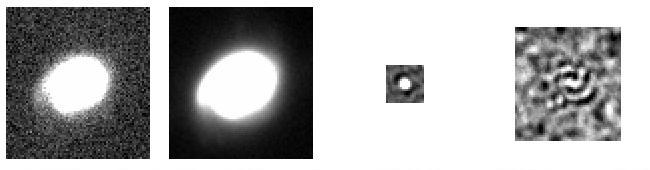
\includegraphics[height=40mm]{figures/conv_crop.jpg}
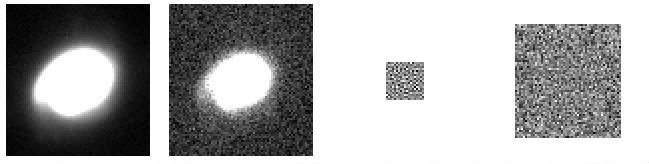
\includegraphics[height=39mm]{figures/dconv_crop.jpg}
\caption{Convolution vs. Deconvolution: The inputs and outputs
from the \code{Kernel} Model I process for a single \code{Footprint}.
For each row, we show from left to right the image that was operated
on, the image it was matched to, the derived \code{Kernel} Model I,
and the associated difference image.  In the top row, we operate on
the noisy science image, yielding a compact \textit{convolution}
\code{Kernel}.  In the bottom row, we operate on the template image 
which has a broader PSF, yielding a \textit{deconvolution}
\code{Kernel}.}
\label{fig-conv}
\end{figure}

Another way to contrast the processes is to look at a histogram of the
residuals in the difference images after the \code{Kernel} Model I
process.  Ideally, the histogram of normalized residuals will be a
normal distribution with a mean of 1.0 and root-mean-square of 1.0.
\Fig{fig-conv-stats} shows these data for the process of
convolving the science image on the left, and deconvolving the
template image on the right.  Each panel shows the histogram of all
\code{Footprint} residuals from a subset of the DC2 images, along with
the idealized normal distribution plotted as a line.  As alluded to
above, the noise distribution on the left has ``heavy tails'', 
which will lead to more spurious high-sigma
detections.  The upshot is that the spatial variation of the
convolution \code{Kernel}s may be compactly modeled.  The figure on
the right shows that the noise is better behaved when operating on the
template images.  However, the method we have chosen to model the
spatial variation of deconvolution \code{Kernel}s for DC2 appears to
fail.

% NOTE TO EDITOR : 
% CAN YOU GET THESE TO LINE UP LEFT TO RIGHT?
% RHL: They are.  What's the problem?
% ACB: I can't see how they turn out since my pdflatex is broken.
\begin{figure}[htbp]
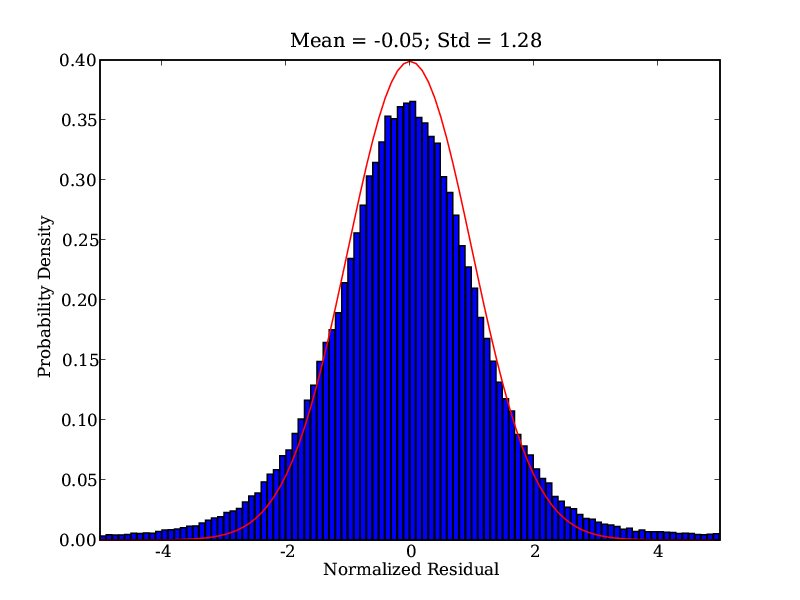
\includegraphics[height=60mm]{figures/sig30Sall.jpg}
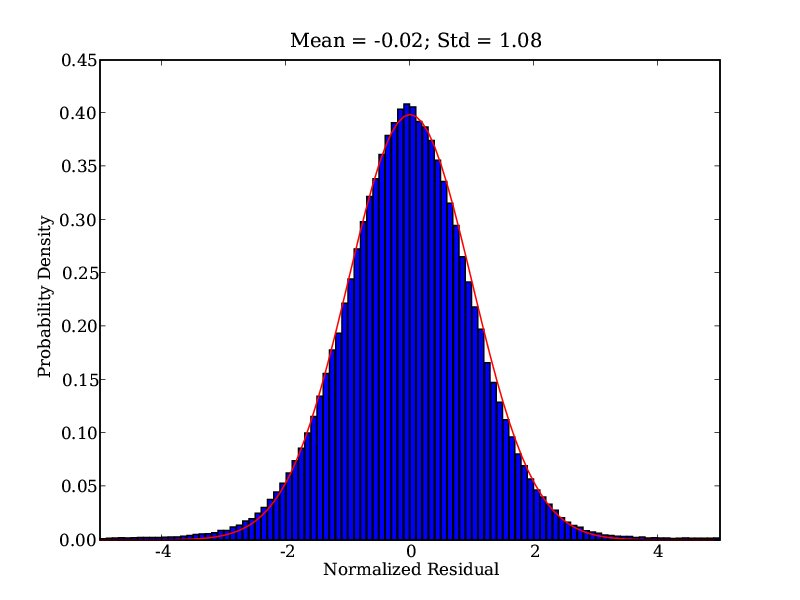
\includegraphics[height=60mm]{figures/sig30all.jpg}
\caption{Histogram of difference image pixel residuals normalized by 
the propagated noise, taken from all \code{Footprint}s after the
\code{Kernel} Model I process.  We plot the idealized normal
distribution as a solid line.  The histogram on the left shows the
results when operating on the science image, resulting in convolution.
The noise is clearly greater than expected.  The histogram on the right shows
the results when operating on the template image, resulting in
deconvolution.  The distribution is much closer to the expected normal
distribution.}
\label{fig-conv-stats}
\end{figure}

\subsubsection{Timing}

The baseline computation estimate for Image Subtraction 
%NOTE:  need reference to document that contains this
is $4.6 \times
10^{-8}$ THz--sec pixel$^{-1}$.  For DC2, we realized a speed of $2.2
\times 10^{-7}$ THz--sec pixel$^{-1}$ with both \code{fw} and
\code{imageproc} compiled with \code{opt=2}.  This is 20\% of the 
required performance.  There are 3 main sections of code that
contribute significantly to the run time: the process of accessing
pixel data; the process of convolving; and the process of filling and
inverting matrices.  The latter two depend implicitly on the first,
each requiring $\code{Footprint}_{\rm Nrow} \times
\code{Footprint}_{\rm Ncol} \times
\code{Kernel}_{\rm Nrow} \times \code{Kernel}_{\rm Ncol}$ pixel 
accesses, making this an important piece of the code to optimize.

%Pixel data are accessed through \code{fw::MaskedPixelAccessors}, which
%in turn call Vision Workbench's
%\code{vw::MemoryStridingPixelAccessor}.  {\bf RUSS - anything to say here?}.

The inverting of matrices is currently done using the \code{vw::math}
interface to \code{LAPACK}.  We are using the \code{pseudoinverse}
functionality to make the inversions more robust.  However, the
computation scaling is more severe for this process than for the less
robust \code{inverse} process.  The scaling for \code{inverse} is
$(\code{Kernel}_{\rm Nrow} \times \code{Kernel}_{\rm Ncol})^2$, while
the \code{pseudoinverse} scales to the 3$^{rd}$ power.  It is thus
important to choose the correct dimensions for our
\code{Kernel}s.  We need them large enough to represent the 
differences in the PSFs, but if we make them too large the above
scaling will start to dominate the computational budget.  There is the
additional complication that as we make the \code{Kernel}s larger, we
need to grow the \code{Footprint}s larger so that there are enough
constraints on the \code{Kernel}; their sizes are intimately
connected.  Current surveys scale the sizes using the image FWHM to
moderate the trade-off between accuracy and speed.

We should also investigate other numerical backends to undertake these
linear algebra operations, including other implementations of BLAS
(e.g.~ATLAS or Goto).  Its unclear if the current \code{LAPACK}
libraries were compiled with optimization; if not, we should realize a
significant speed-up in this processing.

\subsubsection{Issues and Lessons Learned}

The implementation of Image Subtraction for DC2 was very successful,
including stressing the build system with practical software
development, developing framework classes for pixel-level analysis
and linear algebra, and turning the process of image subtraction into
a functional \code{Pipeline}.  However, there remain several
outstanding issues, discussed above, which need to be resolved before
nightly LSST operations.  Many of these will continue on as research
and development tasks during DC3.

\begin{itemize}

\item Regularize \code{Kernel} I. This would have the advantage of 
   damping the noise in the wings of the \code{Kernel} and otherwise
   enforcing smoothness.  However, we would have to be particularly
   careful if the \code{Kernel} needs off-center power (e.g.~to
   compensate for misregistration).  Such smoothing would be
   undesirable for deconvolution \code{Kernel}s.

\item Change the order of \code{Functions}. The software needs to 
   know when there are/are not enough constraints for a given order
   \code{Function}, increasing or decreasing the order of the
   \code{Function} accordingly.

\item Do additional characterization of difference image. This includes 
   detecting and characterizing dipole residuals.

\item Enforce constraint on \code{Kernel} sum. We expect that 
   this number, representing the photometric rescaling, should be
   constant across an entire image but do not enforce this yet.

\item Have more intelligent rejection/retention of \code{Footprint}s.  We 
   will want to make sure that we have constraints for our spatially
   varying \code{Functions} across the entire image, especially in the
   corners.

\item Optimize the size of the \code{Footprint}s and 
   \code{Kernel}s. This includes taking into account the PSF
   full-width-half-maximum and crowding conditions.  In sparse
   fields, \code{Footprint}s that are too large do not add any
   additional constraints on the \code{Kernel} while significantly
   slowing down the processing.  Also, the \code{Kernel} size should
   be larger for poorer seeing data.

\item Consider circular \code{Kernel}s. This would reduce the number of 
   pixels we need for convolution operations by a factor of $\pi$/4,
   although at the cost of extra, possibly expensive, book-keeping.

\item Speed up the code. This includes optimizing convolution, finding 
   more efficient means to address image pixels, and selecting and
   optimizing the compilation of our linear algebra libraries.

\item Improve the spatial \code{Kernel} and background model. We 
   are currently using polynomial functions which can be poorly
   behaved in regions where they are not well constrained.  Options
   include using Chebyshev polynomials.

\item Explore the trade-offs between convolution 
   and deconvolution, and between operating on the science and
   template images.

\item Investigate how to compactly model a spatially varying 
   deconvolution \code{Kernel}.

\end{itemize}

% Subsection 4.2: detection  -*- LaTeX -*-

\subsection{Detection}
\label{Detection}

The object detection and characterization code lies in its own namespace, \code{lsst::detection}.

\subsubsection{C++ Classes}

Detection contains the framework classes related to processing astronomical images.
The fundamental objects are:
\begin{itemize}
\item Source detection
  \begin{itemize}
  \item \code{Threshold}:
    A threshold level.
  \item \code{Footprint}:
    A set of pixels (internally stored as \code{Span}s).
  \item \code{DetectionSet}:
    An STL collection of \code{Footprint}s associated
    with a \code{MaskedImage} (\Sec{FW}).
  \end{itemize}
  
\item Source measurement
  \begin{itemize}
  \item \code{MeasurePixProcFunc}, \code{Measure}:
    Classes designed to measure the properties
    of \code{DiaSource}s.
  \item \code{Peak}:
    A peak in an image.
  \end{itemize}
  
\item Miscellaneous
  \begin{itemize}
  \item \code{BCircle}:
    A description of a circular disk.
  \end{itemize}
  
\item Classes ready for DC3 (\ticket{322})
  \begin{itemize}
  \item \code{PSF}, \code{dgPSF}:
    Place-holders to describe point spread functions.
  \item \code{Defect}:
    A CCD defect, such as a bad column.
  \end{itemize}
\end{itemize}

All of these classes were implemented for DC2, and make use of
the support classes defined in mwi (e.g.~\code{mwi::data::LsstBase},
\code{mwi::utils::Trace}).  They are documented using doxygen,
although the level of the documentation is patchy;  in particular
high level documentation (motivation and examples) tends to be missing.

\paragraph{Source detection}

\subparagraph{Footprint}
The fundamental class in source detection is a \code{Footprint}, a set
of connected pixels above (or below) some threshold. Two pixels are
said to be `connected' if they touch along a side or by a corner.  The
internal representation of a \code{Footprint} is an STL container of
\code{Span}s --- a triple of a row number in the image and a starting
and ending column.\footnote{We are currently schizophrenic as to
  whether such ranges are inclusive or exclusive; \code{Span}s are
  inclusive, while e.g.~\code{vw::BBox2i} is exclusive. We need
  to be consistent in DC3 and beyond.}
The user currently needs to be aware of this; for
DC3 we should provide an iterator over the pixels in a \code{Footprint},
and possibly move \code{Footprint} to \code{fw} (\Sec{FW}).

The threshold defining a \code{Footprint} is a class in its own right,
imaginatively named \code{Threshold}, which may be implicitly
initialised from a numerical value or constructed to be a negative
value (which \code{Footprint}s must lie below), and/or a value
in units of an image's variance or standard deviation.

In DC2 we have been detecting in an unsmoothed image, and demanding
at least a certain number of pixels above/below a threshold.  In general
we wish to search for objects based on a maximum likelihood
analysis of the image;  in the limit of faint sources with
uncorrelated Gaussian noise, this corresponds to smoothing the
image with the assumed shape of the sought-for source (e.g.~with
the PSF).  We have not implemented any such scheme for DC2,
although the machinery is present in \code{fw}'s \code{Kernel}
classes.  The natural generalisation of this approach is to
search in a $\chi^2$ image.  Another question is the actual
value of the threshold to adopt, but this (although an interesting
question) has little impact upon the image processing algorithms
employed.

A \code{Footprint} or set of \code{Footprint}s only makes sense
in the context of an image;  a \code{DetectionSet} associates
an STL container of \code{Footprint}s with a \code{MaskedImage},
and may be constructed from the \code{MaskedImage} and a \code{Threshold};
it is templated over the \code{Image} and \code{Mask} pixel types.

Experience with other surveys has shown that \code{Footprint}s provide
a natural representation of sources;  if the pixel intensities are
stored within the class, a \code{Footprint} may be used to define
a source, even if two or more sources overlap.  We may expect that
\code{Footprint}s will acquire more methods as LSST DM proceeds.


\paragraph{Source measurement}

DC2 only concerns itself with difference imaging, and thus with
\code{DiaSource} (\Sec{FW}).  The current implementation of the source
measurement code uses a functor scheme (class
\code{MeasurePixProcFunc} driven by \code{Measure}) similar to that
used for iterating over \code{Image}s.  This seems appropriate,
certainly for the simple moments that we are measuring in DC2. A
suitable generalisation, possibly iterating over \code{Footprint}s,
should be used in DC3.

\subparagraph{Peak}
An approach to defining object identity is to determine the set
of peaks present in a set of images;  in order to treat blended
sources simultaneously --- as well as to cull noise peaks --- it
is often convenient to treat all peaks present in a \code{Footprint}
together.  The class \code{Peak} was defined to fill this r\^ole,
although it has not been employed in DC2.  

\subsubsection{Classes ready for DC3 (\ticket{322})}

Some functionality is present in the DC2 code base,
although not used in the DC2 processing.

\subparagraph{Interpolation over defects}
A CCD defect, such as a bad column, is described by a \code{Defect};
the list of problems for a given CCD can be read from a \code{Policy}
(\Sec{Policy}) file.  Once identified, and given some information
about the PSF,  these defects are interpolated over using linear
predictive coding (LPC), and labelled as interpolated in the
associated \code{Mask}.  This patching over defects avoids problems with
e.g.~cosmic ray detection code which otherwise detects all bad columns;
it is of course possible to write more complicated algorithms that
handle bad pixels, but it's simpler to interpolate them away.

\subparagraph{PSFs}
We have classes \code{PSF} and \code{dgPSF} (a double-Gaussian
inheriting from \code{PSF}) to describe the PSF.  These are
present purely as placeholders, and to give the \code{Defect}
and cosmic ray code a measure of the seeing.

\subparagraph{Cosmic Rays}
LSST expects to perform cosmic ray (CR) splits, but not all datasets
allow such luxuries, and it is often advantageous to be able to
detect CRs in a single band --- for example, if the two exposures
need to be aligned before CR removal can be attempted.  The current
implementation is based on that used by SDSS and looks for gradients
in the image that exceed the band limit (i.e.~are sharper than
the PSF).  The algorithm seems to work reasonably well on the
Megacam data used in DC2, but may well need work or replacement
for DC3.

\begin{figure}[htbp]
  \begin{center}
    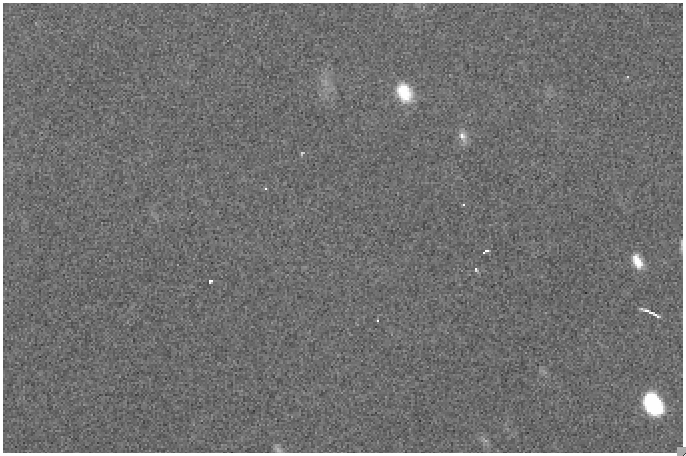
\includegraphics[height=60mm,angle=90]{figures/CR-before}
    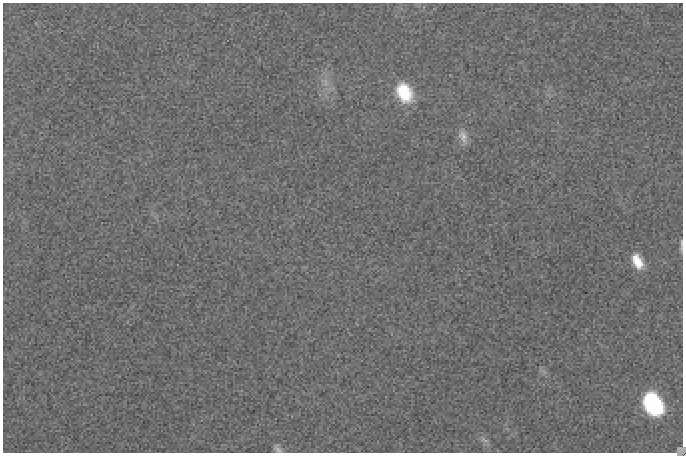
\includegraphics[height=60mm,angle=90]{figures/CR-after}
  \end{center}
\caption{A $343\times228$ pixel portion of a CFHT image (\code{cal-53535-i-797722\_1})
  before (left) and after (right) defect and cosmic ray interpolation. The entire
  $2k\times4k$ image contains approximately 1100 cosmic rays.
}
\label{FigCRbefore}
\end{figure}

% Subsection 4.3: MOPS

\subsection{Moving Object Prediction System (MOPS)}
\label{sApps-mops}

DC2 integrated the night-time functionality of MOPS (``NightMOPS''),
which consists of predicting locations of known objects expected to
appear in images.  This is done concurrently with image processing,
with the intent of concurrently reporting both detected objects and
predicted objects to the Association Pipeline on a per-image basis.
This process is distributed trivially by distributing responsibility
for subsets of the set of known objects between multiple slices in the
NightMOPS Pipeline.

\subsubsection{MOPS Preparations for DC2}
In full LSST, the day-time functionality of MOPS (DayMOPS) involves
processing large sets of detections into a catalogue of orbits.
Additionally, each day DayMOPS will be responsible for making two or
more ephemeris predictions for all known orbits for the coming night.
To prepare a catalogue and collection of ephemerides which was similar
to that expected in full-scale LSST, we fed the Minor Planets Center
catalogue of detections into DayMOPS.  The DayMOPS software generated
a catalogue of 159357 orbits based on 29779380 detections.  Prior to
DC2, three ephemeris points were predicted per orbit, per night for
which we had image data, a total of 87008922 ephemerides.  The
ephemeris points were predicted at midnight, 4 PM before that midnight
and 8 AM after that midnight, and stored in the central LSST database.

\subsubsection{NightMOPS Within DC2}

\paragraph{}
NightMOPS was implemented as an Application Pipeline, implemented
entirely in \code{Python}.  The workload was distributed between
Pipeline Slices, each of which were responsible for subsets of the
total objects.

NightMOPS received its input from the DC2 Harness via the Events
system, which would announce a field of view and time as image
processing for those images began.  On receiving this Event, each
NightMOPS Slice would concurrently query the ephemeris collection
generated by DayMOPS for ephemeris points (and their associated error
ellipses) corresponding to the evening of the image and the Slice's
assigned object IDs.  Slices would then prune objects which would not
pass nearby the field of view at that time and ignored them.  The
positions of the remaining objects were quadratically interpolated
from their three associated ephemerides.  These positions and their
associated object IDs were then passed on to the Association Pipeline
via the persistence framework and the database, with an Event passed
to the Association Pipeline informing it of the availability and
location of the data.


\subsubsection{Results}
NightMOPS predicted 25 objects which were detected in images during
the DC2 runs.  This small number of matches seems to be a result of
the limited number of objects detected in the MPC database and the
areas of sky in the images we chose for DC2.  All of our interpolated
ephemeris locations  were very close to the actual observed
detections, an average of 5.8 arcsec in error.  The maximum
distance between predicted location and observed location was
10 arcsec; the minimum was 1 arcsec.   An example detection of a MOPS
predicted object position is shown in \Fig{MOPSPredImage}.

\begin{figure}[htb]
\begin{center}
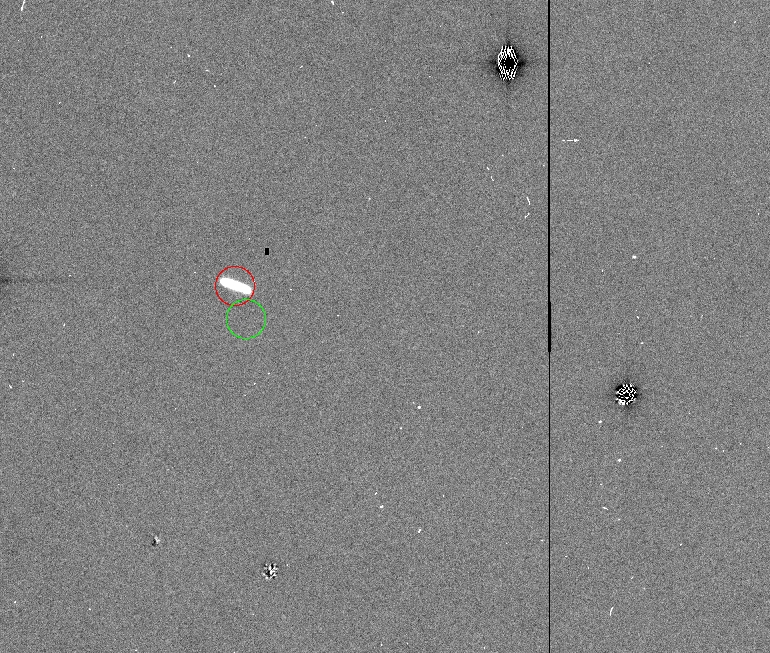
\includegraphics[height=60mm] {figures/MopsPred_rlp0130_705197}
\caption{Detection of a MOPS predicted solar system object in DC2.
The object has orbit\_id=41904, and was detected in Visit 705197.  The
green circle is centered on the predicted position, while the red
circle is centered on the detected position, which is about 6 arcsec away.}
\label{MOPSPredImage}
\end{center}
\end{figure}


%\subsubsection{Performance}
%NUMBERS and some OLD BENCHMARKS
%The majority of this time was dominated by database query and transfer.  This time was relatively small %compared to the time taken by image processing; NightMOPS was far from a bottleneck in DC2.

\subsubsection{Issues and lessons learned}

MOPS proved itself capable of night-time operation which met or
exceeded our performance demands.  Further, the DC2 preparation
demonstrated the functionality of the DayMOPS system for identifying
objects from sets of detections.  Though our number of matches between
ephemeris predictions and observed objects was somewhat small, this
was limited by factors outside of our control, including the currently
limited set of known asteroids.

The most significant problem within NightMOPS was that the predicted
error ellipses for objects were very large (average semi-minor axis:
1806.64 arcsec, average semi-major axis: 2947.12), especially when
contrasted with the average distance from detected object to predicted
ephemeris location (6 arcsec).  We see several possible causes for
this problem, particularly the ephemeris prediction libraries we used
to generate the orbital covariance matrices, which were provided to us
by the NASA Jet Propulsion Laboratory, or our own libraries which
convert from covariance matrices to error ellipses.  We are continuing
to investigate this problem and plan to address it in DC3.


It is also of note that database access time during NightMOPS
operation will likely decrease in the future: in LSST, we will only
need to query a table containing ephemeris for the current night, not
for a large set of nights as in DC2.  Further, small preliminary
experiments have found that changing our SQL query syntax can result
in as much as a fifty-fold increase for NightMOPS database queries.
As database query was the major factor in DC2 performance of
NightMOPS, we can expect NightMOPS to perform far better in DC3 and
full-scale LSST than we observed in DC2.

\subsubsection{Conclusions}
Though the small number of NightMOPS predictions to detected object
matches in DC2 was a small disappointment, DC2 proved a convincing
test of the NightMOPS subsystem, demonstrating both correctness and
high performance.  Further, we can realistically expect massive
improvements in performance, making a strong argument that even as
other Pipelines improve in performance, NightMOPS will not become a
bottleneck.

A further issue related to the JPL code is that it is only licensed
for use within the U.S.~and within the LSST consortium. We are 
exploring options for relaxing these restrictions or replacing
the JPL code with equivalent code (Milani or Tricarico).

% Subsection 4.4: Association

\subsection{Association}
\label{association}

The task of the association pipeline (AP) is to compare information coming 
from the latest telescope visit with historical knowledge of the sky;
specifically, to determine which objects, if any, correspond to the difference 
sources being produced by the detection pipeline (DP) and which of those
sources correspond to the moving objects predicted to be in the field-of-view
(FOV) by the NightMOPS pipeline. These associations provide the basis from
which the alert generation pipeline will decide whether a difference source
constitutes an interesting evolution of some existing object or is evidence
of an entirely new object; i.e. whether or not an alert concerning the source
should be sent out to the astronomical community at large. Keeping the number
of alerts at a manageable level is paramount to their utility --- it follows
that every attempt to avoid repetition in alert content must be made. The
association pipeline therefore not only compares against historical knowledge
of the sky, but also updates this knowledge: new objects for unmatched
difference sources are created and difference sources are archived so that
on future visits to the same FOV, they can be taken into account by the alert
generation rules. For the same reasons, we envision that object attributes may
also be updated according to their associated difference sources.

\subsubsection{Architecture}

The execution of the association pipeline is split into three main phases: a
load phase, a compute phase, and a store phase. The first of these is
concerned with loading historical data for the FOV being observed from disk
into memory, the goal being to allow further computation to proceed with as
few time-consuming disk accesses as possible. Next, the compute phase matches
difference sources to objects and then moving objects to difference sources ---
both matches are purely spatial, and are described in more detail below.
Lastly, the store phase is in charge of updating historical knowledge of the
sky based on the compute phase results.

Given that the LSST object catalog is expected to contain between 14 billion
(DR1) and 49 billion (DR11) objects at roughly 1.7kB per object and that the
AP time budget per visit is only about 10 seconds, the load phase cannot be
implemented na{\"\i}vely; both parallelization and partitioning are employed to
meet performance targets. We first observe that the AP performs purely spatial
matches, so little more than object ID and position are required to feed the
compute phase. These attributes are extracted from the master copy of the
object catalog, which is maintained in a relational database and is supplied
as an input to a DC2 pipeline run. The resulting very thin vertical partition
is stored in the file system to keep database load in check. However, at
several hundred GB the partition remains impractical to read into (or keep in)
memory and spatial partitioning is required for efficient access: objects are
divided into equal height declination stripes, which are then physically
partitioned into chunks of equal width in right ascension. For each chunk, the
AP maintains 2 files: the first contains objects from the original input object
catalog, and the second, a chunk \emph{delta} file, is dedicated to objects that
were created as part of visit processing. The load and store phases only read
and write files for chunks that overlap the visit FOV and the store phase
writes only \emph{delta} files.

Chunks are sized such that the spatial extents of a FOV can be tightly
approximated by a relatively small set of chunks (\ensuremath{\sim}100
for a full 10 deg$^{2}$ LSST FOV), minimizing I/O wasted on objects
lying outside the FOV. This also allows the corresponding files to be
distributed across many disks so that multiple worker slices can be used
to read and write them in parallel. Unfortunately, one problem arises from
this strategy: spatial matches are run in the pipeline master process in
order to avoid slice-to-slice communication, a capability not
supported by the DC2 pipeline framework. To see why slice-to-slice
communication would be necessary if different slices handled matching for
different parts of the sky, consider that a single difference source might
match objects read by different slices. But running the compute phase
in the master means that worker slices must somehow communicate data they've
read back to the master. This is again a feature not fully implemented by the
DC2 pipeline framework. To circumvent these limitations, AP worker slices read
files into a shared memory region accessible to all other workers, as well as
the master. This works well but constrains the AP to scale within the bounds
of a single machine.

Finally, it should be noted that the alert generation pipeline (AGP) will
peruse much more than just a few attributes of each object and difference
source: it is envisioned that each object matching a difference source as
well as all historical difference sources associated with each matched object
will be thoroughly examined. Accesses will be made to database tables rather
than custom files, and are sparse if na{\"\i}ve spatial clustering is employed: the
up to \ensuremath{\sim}10$^{5}$ difference sources will match objects scattered
amongst up to 10$^{7}$ objects in the FOV. Though we expect that at most
\ensuremath{\sim}500MB of object data must be read into memory for
examination, and at most 300MB written, sparsely laid out objects would
require either a large number of disk seeks or sequential reads of many times
more data. In either case, parallelization over an inordinately large number
of disks would be required for reasonable performance. We plan to address this
issue by splitting the object table into two: one table for known variable
objects and one for the rest. Since almost all difference sources are expected
to match known variables, spatially clustering the variable object table will
result in a dense layout of matched objects on disk, allowing much more
effective use of I/O. Also, instead of loading variable objects during the 10
second AP time-window, they can be pre-loaded as soon as the FOV is known,
either by explicit inserts into an in-memory table or by issuing queries to
warm up database caches. As the AGP is out of scope for DC2, this aspect of
the AP is currently not implemented.

\subsubsection{Test Platform and Data Volume}

The AP was tested on a server with two Intel Xeon E5335 2.0GHz CPUs
and 16GB of RAM, running Red Hat Enterprise Linux AS release 4. The AP was
compiled without optimization (-O0) and a single 1 deg$^{2}$ FOV
containing 417,327 objects was used as input. This FOV overlapped ~25 chunks,
of which only 16 were non-empty. Analysis was performed using DC2 runs
rlp0128 and rlp0130, for which per-visit maximums of 5086 difference
sources and 22 moving object predictions were recorded. The worst-case figures
for full-scale LSST are expected to be roughly 20 times larger: we will be
dealing with up to 10$^{7}$ objects, 10$^{5}$ difference sources and a few
thousand moving object predictions in a single FOV.

\subsubsection{Implementation and Performance}

\paragraph{Load Phase}

A single worker Slice was used to read the roughly 15MB of data contained in
the DC2 chunk files into memory. Due to last-minute problems with Lustre
parallel file system configuration, chunk files were stored on an NFS volume:
the very same volume containing exposure data operated on by the
image-processing pipeline. The fact that the DC2 pipeline repeatedly visited
the same FOV (virtually guaranteeing that chunk files were read from cache
rather than disk) and the use of a contended NFS volume for storage
invalidates DC2 timing results for this part of the load phase. However, by
running tests in which the DC2 chunk files were loaded from dedicated SAS
disk, these reads have been confirmed to complete in less than one second.

Once objects for the field-of-view have been loaded, they are indexed into a
data structure that supports the very fast proximity searches required by the
spatial matches of the compute phase. Index construction duties are assigned
to the load phase since there are no dependencies on data produced by other
nightly pipelines --- the index can therefore be built while image processing
and detection are running, rather than counting against the 10 second AP time
budget. The data structure is built by bucket sorting objects on declination,
giving a set of very fine declination stripes dubbed zones, and then sorting
objects on right ascension within each zone. In total, a single thread takes
\ensuremath{\sim}0.3 seconds to produce an index for the 417,327 objects in
the DC2 input object catalog. Though the complexity of sorting objects within
a zone is O(N log N) where N is the number of objects in a zone, the dominant
costs in index construction are linear-time. Tests have been run in which 3.6
million objects were indexed in \ensuremath{\sim}2.8 seconds by a single
thread on a SunFire V240 (16GB RAM, 2 UltraSPARC IIIi 1.5GHz CPUs), so scaling
up the number of objects by a factor of 10 to 20 from DC2 levels is not
expected to be problematic. Nevertheless, if performance becomes an issue then
index construction can be parallelized.

\paragraph{Compute Phase}

After index creation, the AP load phase is finished and the AP waits for the 
DP to signal its completion via an event. Once this event is received, the AP
reads the difference sources stored in the database by the DP into memory.
In DC2, this took \ensuremath{\sim}0.12 seconds for every thousand difference
sources read in, peaking at \ensuremath{\sim}0.6 seconds for 5000 difference
sources. In production, 10$^{5}$ difference sources must be handled in the worst
case: taking 12 seconds to read them into memory is unacceptable. Luckily,
multiple opportunities for optimization on this front exist: first of all,
the AP currently retrieves all attributes of difference sources, even
though it uses only position and id. Secondly, database access occurs through
a wrapper for a debug build of the CORAL database access library, adding 
multiple layers of indirection on top of the native database API --- for DC3,
the LSST database access wrapper will call native APIs directly. Finally, if
these optimizations do not yield the necessary speed-ups, we plan to
parallelize difference source reads.

With difference sources for the visit in hand, the AP is ready to perform its
first spatial match, the task being to find all objects within a fixed
distance $R$ (DC2: 0.5 arcsec) of each difference source. This is 
accomplished by using the object index created in the load phase: each zone
in the index is chosen to correspond to a declination range slightly larger
than $R$ so that for any given difference source position $P$, potential
matches must be in one of 3 zones: the zone containing $P$ and the those
immediately above and below. In addition, for each zone in the index a
constant $\alpha$ is pre-computed such that any 2 points in the zone separated
by more than $\alpha$ in right ascension must be separated by distance at
least $R$. So, by searching for objects lying in one of 3 zones and that have
right ascension within $\alpha$ of $P$ (which can be done with binary search
since objects are sorted on right ascension within each zone) we quickly
obtain a tight set of match candidates from which objects further than $R$
from $P$ are easily removed. As a further optimization, we organize difference
sources into a zone index and process them one zone at a time, in right
ascension order within each zone. As a result, successive proximity searches
exhibit good spatial locality; given the spatial organization of data in zone
indexes, this translates to good memory locality.

Building a zone index for between 772 and 5086 difference sources took
from 0.8 to 5 milliseconds; elapsed time was roughly linear in the number of
difference sources inserted into the index. Matching then took between 1.5
milliseconds and 0.13 seconds, with most matches finishing in under 3
milliseconds. We suspect the spikes in match timing are due to the spatial
distribution of difference sources in particular visits, though this remains
a topic of investigation for DC3. Between 182 and 2243 difference source to
object matches were found; these were written to the database in 0.02 to 0.063
seconds, with timing linear in the number of matches.

At this point, the AP waits for an event signaling that NightMOPS has finished
predicting which moving objects will appear in the visit FOV. As soon as this
event is received, predictions are loaded from the database --- for DC2 runs
under consideration, a maximum of 22 predictions per-visit were retrieved in
roughly 0.015 seconds. Predictions with positional error ellipse semi-major
axis length greater than 3 deg were discarded; the rest had both semi-major
and semi-minor axis lengths clamped to 10 arcsec to avoid producing
thousands of matches for the very large NightMOPS error ellipses. For each
prediction, all difference sources not matching a known variable object and
lying within the predictions error ellipse are found using a modified version
of the spatial match algorithm described above. Match candidates are
identified by computing a per-prediction error ellipse bounding box (in zone
number and right ascension) and then using the difference source zone index
created for the previous match to look them up. The scarcity of moving objects
and error ellipse clamping led to sub-millisecond DC2 timings for this part of
the compute phase.

Finally, difference sources that will generate new objects are identified by
scanning all sources and flagging those not matching any object; identifiers
for flagged sources are then stored in the database. Both operations take time
linear in the number of difference sources involved: in DC2, 230 to 2294 new
objects were identified in 0.4 to 4 milliseconds and persisted in 0.011 to
0.067 seconds. Lastly, the results of matching moving object predictions to
difference sources are persisted; this took 0.018 seconds on average --- no more
than 4 matches were found in a visit.

\paragraph{Store Phase}

With the results of the compute phase stored in per-visit database tables, the
final task of the AP is to update historical knowledge of the sky. This
process begins by writing out delta files for chunks overlapping the
visit FOV. DC2 timings for this step, executed on a single worker slice,
varied from 0.1 to 1 seconds. Swings in timing were caused by NFS contention ---
the AP was often finishing a visit just as the image processing pipeline was
loading science and template exposures for a subsequent visit. Further tests
in which delta files were stored to dedicated disk revealed that these writes
very consistently took between 0.6 and 0.7 seconds for about 1.3MB of data.

Following delta file writes, a series of MySQL scripts are fired off. The
first of these uses the match result tables to update the \code{Object} table:
currently only the time of last observation and observation count in each
filter is updated. The script also creates new objects from difference sources
and sets the \code{objectId} of each difference source to the id of the
closest matching object or the object created from it. Finally, it appends
difference sources to the \code{DIASource} table. DC2 execution times for this
script were either short or long: between 0.35 and 4.6 seconds, with only
very few visits taking time between the two extremes. Furthermore, we found
that the execution times for the SQL statements in the script as reported by
MySQL consistently added up to significantly less than the total run-time of
the script.

The second script appends per-visit match results and NightMOPS predictions 
to historical tables. This allows for debugging without littering a run
database with hundreds of small tables, and can be toggled on or off using a
policy file flag. The last script simply drops all visit specific tables
created by DC2 pipelines and is again controllable via policy. These two
scripts exhibit similar behavior to the first: execution time was quite large
(3--4.5 sec, except for the last visit in a run, which took 0.15 sec) but
timings for the individual statements as reported by MySQL do not add up. The
cause of these discrepancies remains unclear --- we plan to investigate and
address this issue in DC3.

\subsubsection{Conclusions and Future Work}

In total, the AP completed in 1.5 to 10.0 seconds per visit, averaging 7.4
seconds with the vast majority of time spent in MySQL scripts that update the
database at the end of a visit. Despite the use of a single-host NFS
filesystem for disk storage and MySQL performance anomalies in the store
phase, performance targets were either met or exceeded for all 62 visits
under consideration, convincingly demonstrating the feasibility of the AP
design for full scale LSST data volumes.

Features to be implemented and/or investigated in the DC3 timeframe include:
\begin{itemize}
\item \emph{Expanded Python Interface}:
    The AP currently exports a very minimal Python interface. For DC3 we
    will expose the spatial matching algorithms to other pipelines which
    require similar functionality.
\item \emph{Probabilistic Matching}:
    Positional error ellipses for both objects and difference sources are
    available. Given a difference source matching multiple objects, these
    can be used to pick the best matching object according to probabilistic
    criteria (rather than simply picking the closest one). Alternatively
    or in addition, all difference source to object matches could be
    officially stored for later perusal.
\item \emph{Proper Motion Correction}:
    By storing proper motions along with object positions in chunk files,
    object positions can be extrapolated to the times at which visits actually
    occur (and at which difference source positions are measured), thereby
    improving match accuracy. This extrapolation can be done by the load phase
    and overlapped with disk I/O. It incurs minor computational costs, and scales
    linearly in the number of objects.
\item \emph{Correction for Refractive Effects}:
    Also expected to have a significant impact on object positions are
    color dependent refractive atmospheric effects. Using stored
    colors for each object and the zenith angle for the visit, we expect
    to be able to meaningfully improve the object positions used as input to
    the spatial match routines.
\item \emph{Transactions and Data Volume}:
    We hope to investigate the feasibility of updating the database and chunk
    files in transactional fashion with visit-level granularity, so that from
    a database perspective each visit appears to have either completed
    successfully or not at all. We also plan to run tests in which the input
    \code{Object} catalog is significantly larger than the one used for DC2;
    the goal will be to stress the I/O intensive portions of the AP with a
    particular focus on more fully characterizing the performance of the
    store phase.
\end{itemize}

Some of the proposed DC3 tasks will result in a significant size increase of
chunk files --- brightnesses and position errors will need to be stored in the
filesystem. Besides potentially complicating the process by which chunk
files and the database are kept in-sync, increased demands will be placed on
I/O and computational subsystems. Though we do not expect these to overwhelm
the capabilities of a single server, we observe that future iterations of the
AP may yet again increase these demands, especially as the design and
requirements of the alert generation pipeline solidify. We therefore plan to
re-implement the AP in terms of the slice-to-master and slice-to-slice
communication primitives which are expected to be provided by the DC3 pipeline
framework. This will improve AP scalability and has the added benefit of
allowing the (relatively complicated) shared memory management code to be
excised, significantly simplifying the AP implementation.



% -- Section 6
% section 5: Results

\section{Results}

\subsection{Summary of DC2 runs}

In the course of executing DC2, we ran the pipelines over our input data
numerous times.  These runs uncovered a variety of bugs, performance
problems, and data quality issues which led to additional improvements
to the code.  Eventually, the maturity of the system was sufficient to
produce runs that would meet our objectives, so we have focused our
analysis of the results on three particular runs that featured
identical versions of the software: \code{rlp0127}, \code{rlp0128}, and 
\code{rlp0130}.  In these runs, the Image Processing and Detection
(IPD) pipeline featured 1 master pipeline process and 36 slice process
running across six nodes of the cluster.  The Moving Objects
Prediction System (MOPS) pipeline ran on node 9 with 3 slice
processes.  The Association pipeline ran on node 10 (where the
database was located) entirely in one process, the master process.
Each of these runs operated on a different set of 36 amplifier-sized
images from the same set of mosaic CFHT-LS D4 exposures (amplifier
numbers 73--108, 37--72, and 181--214, respectively).  From a total of
288 possible amplifier images per exposure, the amplifier sets were
chosen to sample different areas of the focal plan; \Fig{f6-1}
illustrates the location of these amplifier sets.  The number of 
visits completed in each run were 53, 62, and 62, respectively, for a
total of 177 visits.   A summary of the three runs, including the
number of images successfully processed, appears in \Table{t6-1}.  

\begin{figure}[htbp]
\begin{center}
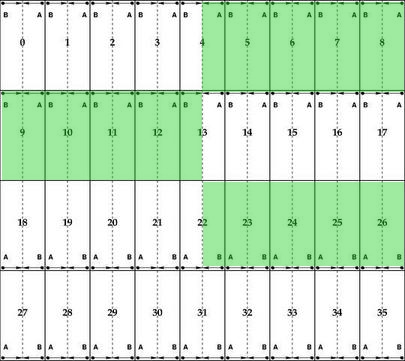
\includegraphics[height=60mm] {figures/MegaCamMap}
\caption{Map of the CFHT MegaCam focalplane.  The area covered by DC2
  runs rlp0127, rlp0128, and rlp0130 are shown in green\label{f6-1}}
\label{FigMegaCamMap}
\end{center}
\end{figure}

\begin{table}[htbp]
\begin{center}
\caption{Summary of DC2 Reference Runs\label{t6-1}}
\vspace{\baselineskip}
\begin{tabular}{ | r | r | r | c | r | r | r |}
\hline
runId & nVisits & nAmps & Amp IDs & inputImages & outputImages & outputFrac \\ \hline
rlp0127 & 53 &  36 &  73-108 & 1908 & 1875 & 0.983 \\ \hline
rlp0128 & 62 &  36 &  37-72  & 2232 & 2228 & 0.998  \\ \hline
rlp0130 & 62 &  36 & 181-214 & 2232 & 2213 & 0.991 \\ \hline
Total   & --- & 108 &   ---    & 6372 & 6316 & 0.991 \\ \hline
\hline
\end{tabular}
\end{center}
\end{table}

We note that the DC2 pipeline will run without modification on much
larger clusters.  A cluster with 288 cores would allow the full CFHT
MegaCam mosaic to be processed in parallel.  We expect such hardware
to be available to us very soon, and we will supplement this report
with results from such runs when they are available.

\subsection{Science data quality}
\label{ScienceDataQuality}

We did not set explicit science data quality criteria for DC2.
Nonetheless, it is valuable to briefly consider the topic here, since it gives
us guidance in planning for DC3.  The main role of the nightly
processing pipelines in the overall LSST data flow is to generate
transient alerts.  These alerts will be based on the DIASources produced by
the IPD pipeline and associated with Objects by the Association
pipeline. Although the alert generation logic is still to be designed,
it is clear that it will rely in part on the lightcurves of candidate
Objects, since they give the history of the Object's behavior.  A key
science metric, therefore, is the quality of these lightcurves.

Taking the results from rlp0128 as representative of the three runs
that made up DC2, a total of 72569 DIASources were generated.  The
histogram of the number of DIASources per Visit is shown in \Fig{FigDIAHist},
and of the number of lightcurve points for an Object in \Fig{FigDIALCHist}.  Two
points are clear from these plots:

\begin{itemize}
\item{A few visits generate anomalously large numbers of DIASources; and}
\item{The vast majority of Objects have only a single lightcurve point.}
\end{itemize}

\begin{figure}[htbp]
\begin{center}
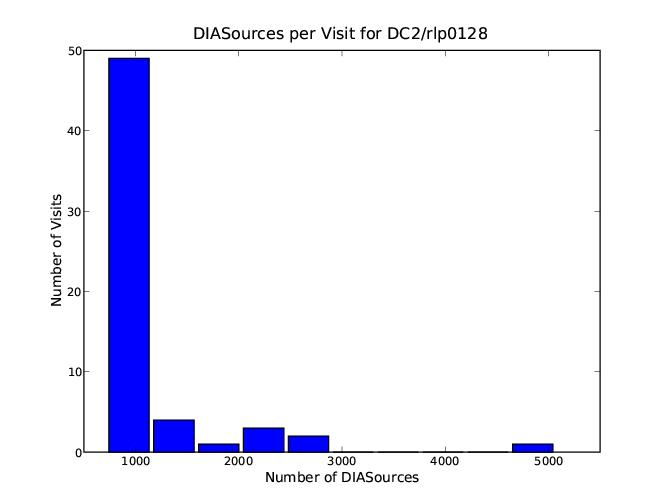
\includegraphics[height=60mm] {figures/VisitHisto_rlp0128}
\caption{Histogram of the number of DIASources per Visit for DC2 run \code{rlp0128}
\label{FigDIAHist}}

\vspace{0.1\textheight}

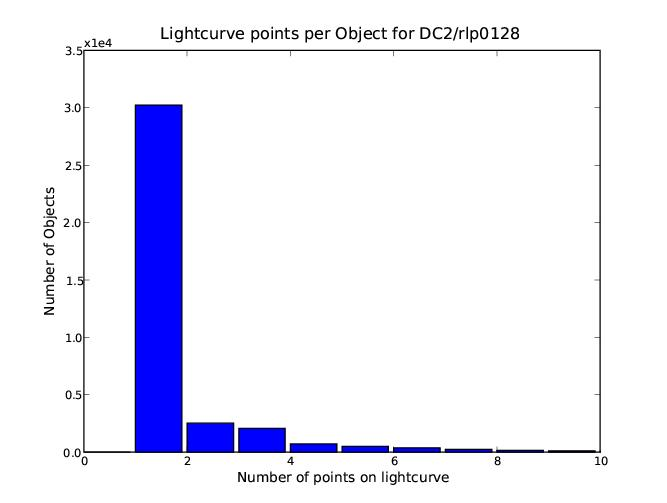
\includegraphics[height=60mm] {figures/LCHisto_rlp0128}
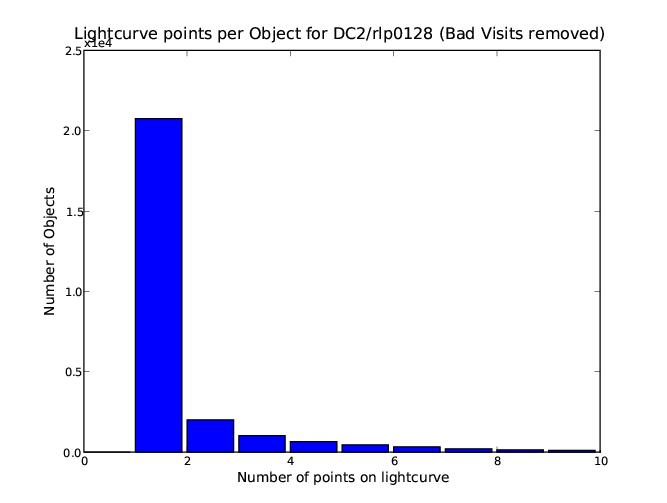
\includegraphics[height=60mm] {figures/LCHistoClean_rlp0128}
\caption{Histogram of the number of DIASources per Object for DC2 run
  \code{rlp0128}.  This is the number of points on the lightcurve for the
  Object. On the right, after eliminating Visits that produced more than 2000 DIASources.
  Note that the ordinate is in units of $10^4$.
\label{FigDIALCHist}}
\end{center}
\end{figure}
  
Inspection of the images shows that the anomalous Visits reflect a
variety of problems in the input images themselves, or in the
subtraction process.   These include template images that are severely
misregistered with their science image. A replot of the lightcurve
point histogram with anomalous Visits (defined as those producing \ensuremath$>2000$
 DIASources) is shown in \Fig{FigDIALCHist}.   There are substantial
reductions in the number of lightcurves with 1, 2, or 3 points, but
qualitatively the picture is unchanged.

Analysis of individual lightcurve quality is time consuming, since the
image region corresponding to each individual point must be assessed
(at the moment, by eye).   At present, only a small fraction of the
available lightcurves have been checked, drawn from representative
points on the  \Fig{FigDIALCHist} histograms, leading to the following
preliminary conclusions:

\begin{itemize}
\item Lightcurves with only a single point are overwhelmingly due to
  cosmic rays.  These will be effectively eliminated in DC3 by
  incorporating cosmic ray rejection into the detection stage of the
  IPD pipeline (cf. \Fig{FigCRbefore}), and further in LSST by the use of two Exposures per
  Visit.
\item The majority of the remaining lightcurves come from ``bipolar''
  subtractions, in which the subtracted image contains a closely
  spaced pair of peaks, one positive and the other negative.   These
  result from poor subtraction kernels.  A number of causes of these
  are understood, and discussed in \Sec{sApp-imsub}.
\item A small number of lightcurves resulting from variable stars are
  present in the data.   The individual DIASources are being correctly
  associated with their Object by the Association pipeline.  The
  fluxes being produced by the Detection stage of the IPD pipeline
  appear to be noisy, however.  Some causes of this are also discussed
  in \Sec{sApp-imsub}.
\end{itemize}

\subsection{Timing results}
\label{sRes-time}

Because the Logging framework attaches a timestamp to every logging
message, we can use it to instrument the pipeline harness and
calculate the time spent in various parts of the pipeline.  In
particular, we inserted logging calls to mark the beginning and end of
important sections of the pipeline processing, such as the start and
end of the process function for each stage.  This technique allowed us
to separate out the different contributions to the overall processing
time, including I/O, middleware overhead, and time spent running
scientific algorithms.  This section presents the results of this
analysis.  

Among the logging markers we included in the harness code was a mark
indicating the start of processing of each visit.  Thus the total cost
of processing each visit was determined by calculating the time
between each such mark.  The average of these times are shown in Table
\ref{t6-2}.  As we will see, the variation is not Gaussian (as they are
certainly dominated by systematic effects), so the calculated standard
deviation is just indicative of the spread in values.\placetable{t6-2}
The variation is better seen in the \Fig{f6-4}.  

\begin{deluxetable}{lrr}
\tablecaption{Average time to process one visit through each pipeline.\label{t6-2}}
\tablewidth{0pt}
\tablehead{
\colhead{Pipeline} & \colhead{avg. time (s)} & \colhead{$3\sigma$ (s)}
}
\startdata
Image Processing/Detection (IPD) &  207.2 & 108.2 \\
Moving Objects (MOPS)            &   52.9 &   4.1 \\
Association                      &  207.4 & 108.5 \\
\enddata
\\[-1.5\baselineskip]
\tablecomments{$N_{visits}=177$}
\end{deluxetable}

\begin{figure}[htbp]
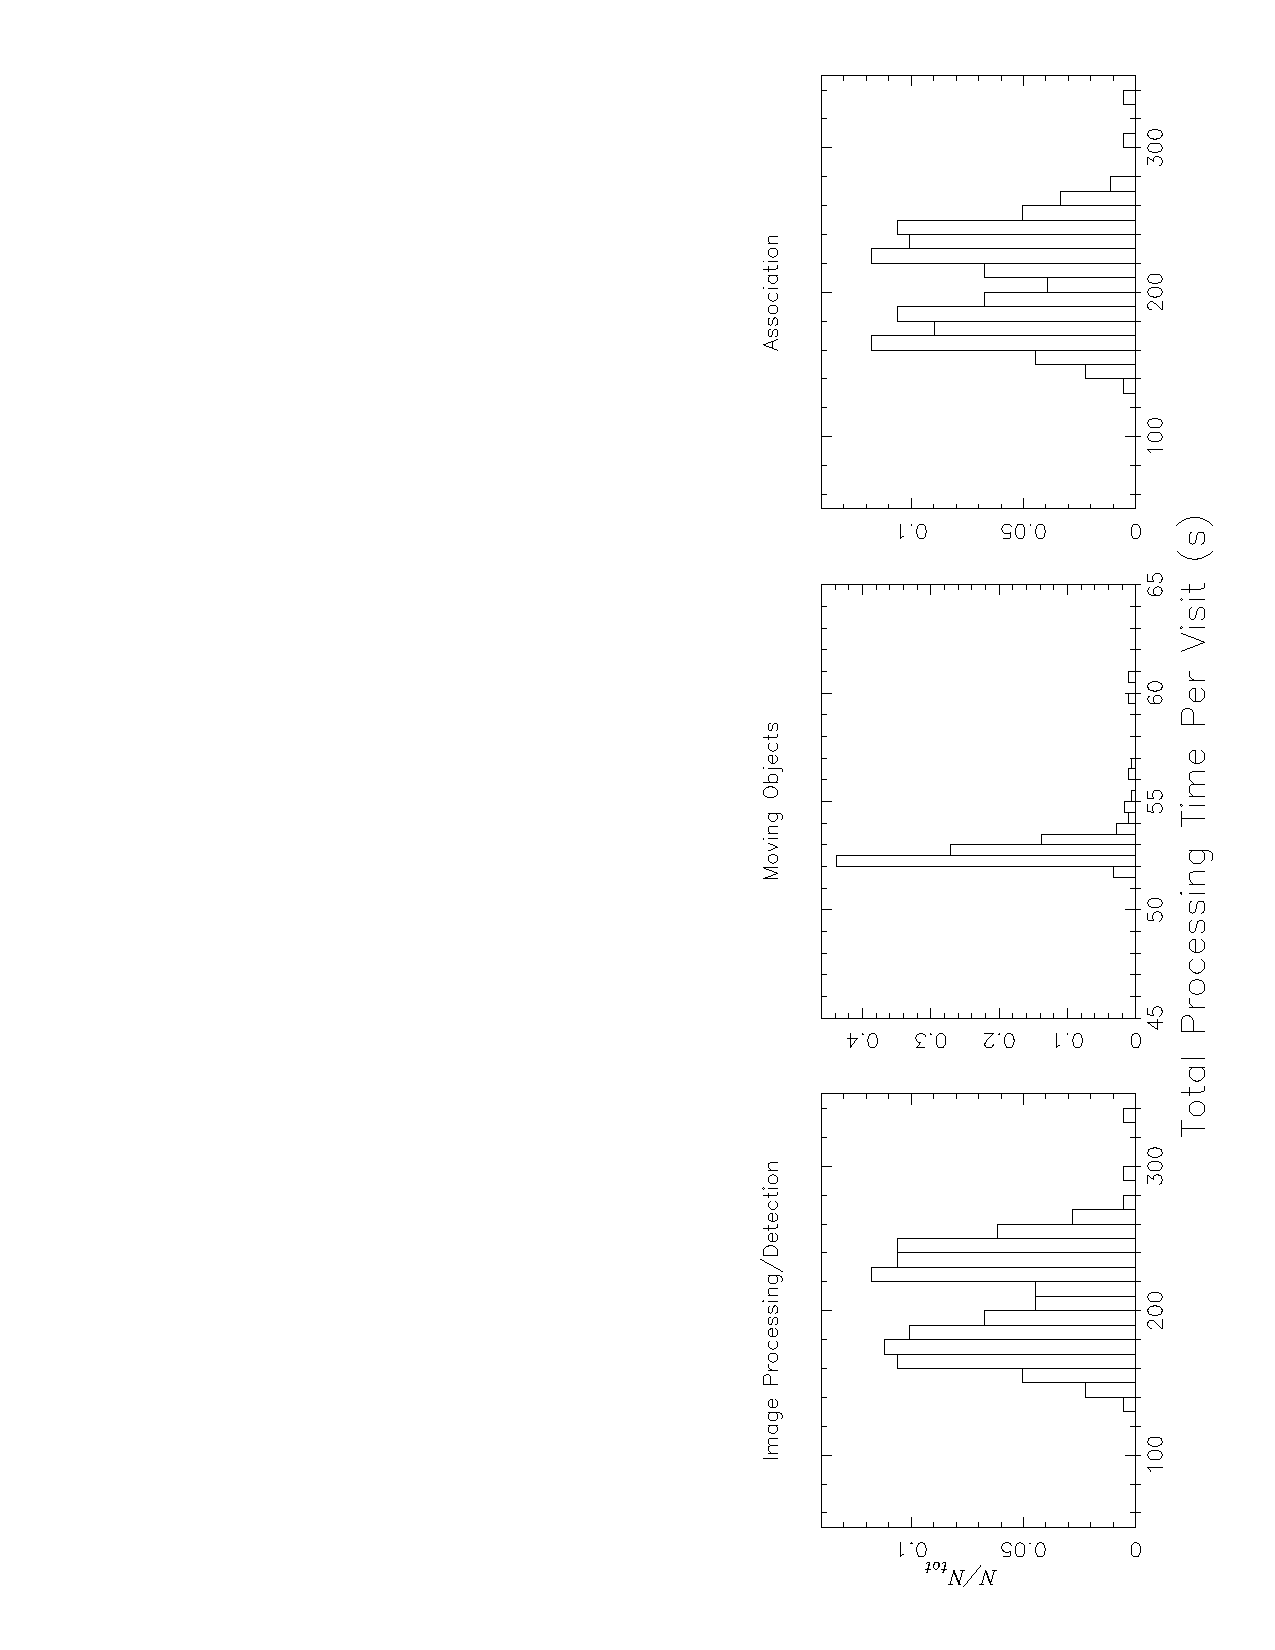
\includegraphics[width=0.8\textwidth,angle=-90,scale=0.375,viewport=364 29 583 757,clip]{figures/MasterLoopHist.pdf}
\caption{Histogram of the times to process each of visit.  The
  $y$-axis measures the fraction of the 177 visits in each time bin.\label{f6-4}} 
\end{figure}

One of the most notable features of the graphs is the correlation
between the IPD data and the Association data.  This reflects the fact
that the Association pipeline pauses at the beginning of each visit to
await an event sent from the IPD pipeline in its last stage signalling
the availability of new detections.  Consequently, the total time spent
processing a visit in the Association pipeline is dominated by this
wait time.  \Fig{f6-5} illustrates only the time spent in
Association application code.  The time spent by the pipeline
framework managing the pipeline, including the spent waiting for
events, has been excluded.  As we can see, this time is much less than
that shown in \Fig{f6-4}.  (As we will see later, the contribution of
the middleware overhead is even smaller.)  The mean time of this set
is 6.9~s.  

\begin{figure}[htbp]
\begin{center}
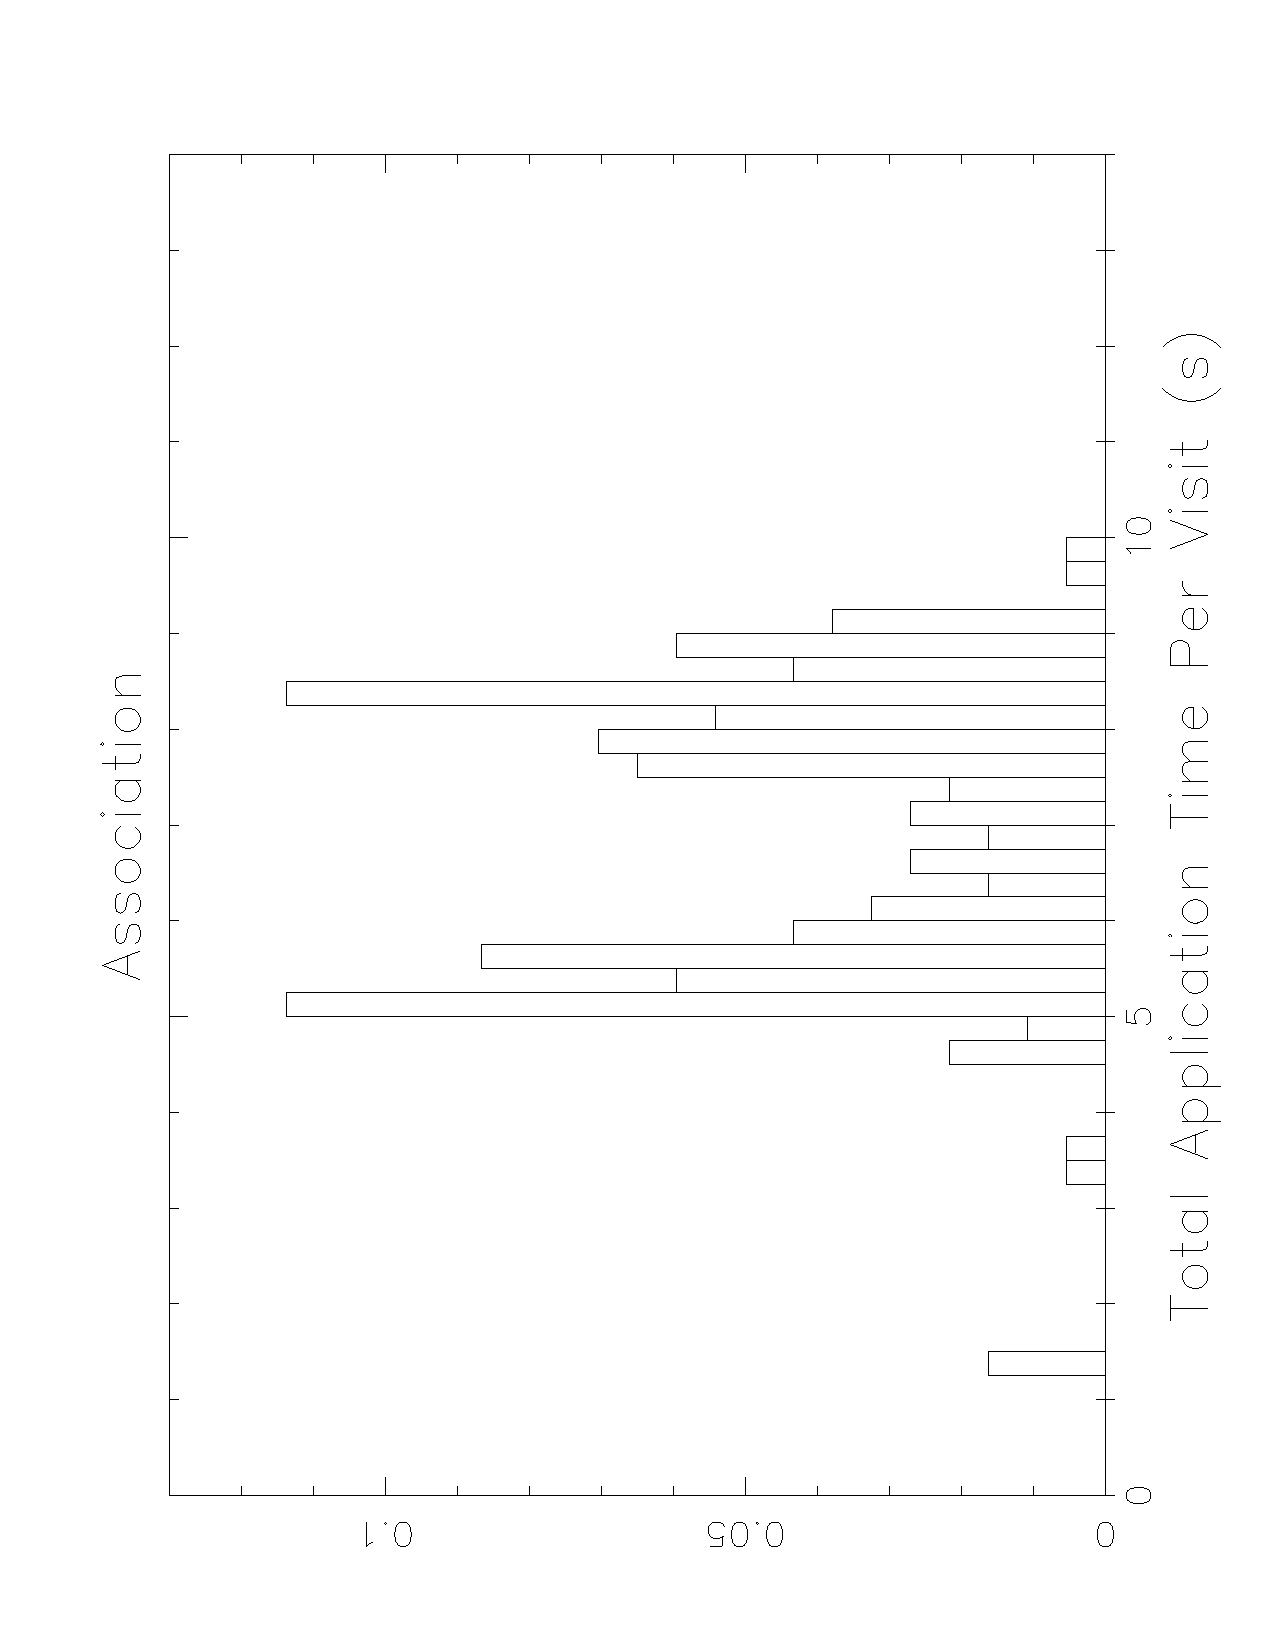
\includegraphics[width=0.8\textwidth,angle=-90,scale=0.45,viewport=47 49 587 719,clip]{figures/AppLoopHistAssoc.pdf}
\end{center}
\caption{Histogram of the times applying the association algorithm to
  each visit, excluding the time waiting for an event and the time
  spent managing the pipeline.  The $y$-axis measures the fraction of 
  the 177 visits in each time bin.\label{f6-5}} 
\end{figure}

\begin{table}[htbp]
\begin{center}
\caption{Average application processing time per stage (s)}
\label{t6-3}
\vspace{\baselineskip}
\begin{tabular}{crccrcr|crcr|crcr}
\tableline\tableline
&&& \multicolumn{4}{c|}{IPD} & 
    \multicolumn{4}{c|}{MOPS} & 
    \multicolumn{4}{c}{Association} \\
\multicolumn{3}{c}{Stage} 
&\multicolumn{3}{c}{average}&\multicolumn{1}{c|}{$3\sigma$} 
&\multicolumn{3}{c}{average}&\multicolumn{1}{c|}{$3\sigma$} 
&\multicolumn{3}{c}{average}&\multicolumn{1}{c}{$3\sigma$} \\
\tableline
& 1 && &   0.023 &&  0.082 & 
       &   0.010 &&  0.008 &
       &   0.460 &&  0.162   \\
& 2 && &   9.567 &&  2.598 &
       &  52.399 &&  2.886 &
       &   0.156 &&  0.210   \\
& 3 && &   0.027 &&  0.015 & 
       &   0.039 &&  0.144 &
       &   0.024 &&  0.040   \\
& 4 && &   0.039 &&  0.007 & 
       &   0.056 &&  0.022 &
       &   0.040 &&  0.024   \\
& 5 && &   7.023 &&  2.411 &&&&&
       &   0.018 &&  0.004   \\
& 6 && & 175.141 && 99.467 &&&&&
       &   0.018 &&  0.005  \\
& 7 && &   6.489 &&  2.016 &&&&&
       &   0.037 &&  0.023  \\
& 8 && &   7.521 && 35.196 &&&&&
       &   6.136 &&  4.741  \\
& 9 && &   0.133 &&  1.119 &&&&& &&& \\
&10 && &   0.061 &&  0.008 &&&&& &&& \\ 
\tableline
\end{tabular}
\end{center}
\end{table}

The obvious conclusion from the results shown thus far is that the
IPD pipeline is the source of the most costly processing.  We narrow
down the source of the bottlenecks in \Table{t6-3} in which we
plot the processing time as a function of pipeline stage for each
pipeline.  From this table, we can see:
\begin{itemize}
\item The costliest stage of the IPD pipeline is stage 6 that does
  the image subtraction.  
\item The next costliest IPD stage, on average, is stage 2 that
  reads the input images into memory; however, the time spent in stage
  7 which does source detection can vary quite a bit, sometimes
  dominating over stage 2.  This depends on the number of sources
  detected in the subtracted image. In the worst cases the subtraction
  was such that the detected sources comprised most of the pixels
  in the image.
\item Stage 2 of the MOPS pipeline is where the ``day-MOPS'' algorithm
  is applied (as the others handle I/O), so as expected this stage
  dominates the processing costs.  
\item The dominant stage of the association pipeline is Stage 8 which
  updates the source catalog.  
\item The association pipelines source matching stages, 3 and 6, are
  relatively fast, typically taking under 0.1 s.  
\end{itemize}

Because the image subtraction contributes such a large fraction of the
overall run time, we undertook a more detailed analysis of its time
usage.  This indicates that the convolution of the template image with
the spatially varying kernel is taking the bulk of the time.   A
simple convolution test case with a spatially invariant kernel
indicates that the current code is running at least a factor of 10
slower than is achieved by existing optimized convolution codes.  We are
working to understand the causes of this, which are certainly
connected to the compiler's treatment of pixel access in the vw
library.  We fully expect to attain full performance from relatively
minor modifications to the vw code, possibly combined with some
changes in the way we utilize it for convolution.

The time spent in stage 6 of the IPD pipeline is dominated by the 
\code{process()} step.  More precisely, because all of the slices
synchronize at the end of this step --- that is, the master process waits
until all of the slices have finished their processing before
proceeding on to the \code{post-process()} step --- the total time spent
in the stage is always longer than the processing time of the slowest
slice.  Looking at all the times spent in the \code{process()} step of
stage 6, we see a large variation.  \Fig{average-node-time} shows the
average time spent on this step as a function of node.  Clearly the
best performing nodes are 5--8 which are the newest machines in the
cluster.  The slices on the older node 1 ran over twice as slow on
average as those on the newer node, and the slices on node 4 ran about
50\% slower.  We might surmise that if we had a homogeneous cluster
consisting all of the newer blades we would see IPD running on average
about 70 s per visit.  We note that the variation of processing times
is still quite large for slices on the newer nodes, suggesting that
peculiarities in the data itself can still have a big effect on the
processing time.

To confirm our hypothesis regarding a homogeneous cluster, we did a
run in which the IPD pipeline only used nodes 5--8.  The average time
spent on image subtraction was 72.7~seconds (with a full range of 33.5
to 122.4~seconds) which is consistent with \Fig{average-node-time}.
The variation is still large, and at least one slice significantly
slows down the processing of the entire exposure.  This could be due
to variations in the data itself, or it could be an effect of running
multiple slices on the same multi-core node.  This latter possibility
could be tested by examining how the processing times change as a
function of the ratio of the number of slices deployed on a node
vs. the number of available cores.  

\begin{figure}[htbp]
\begin{center}
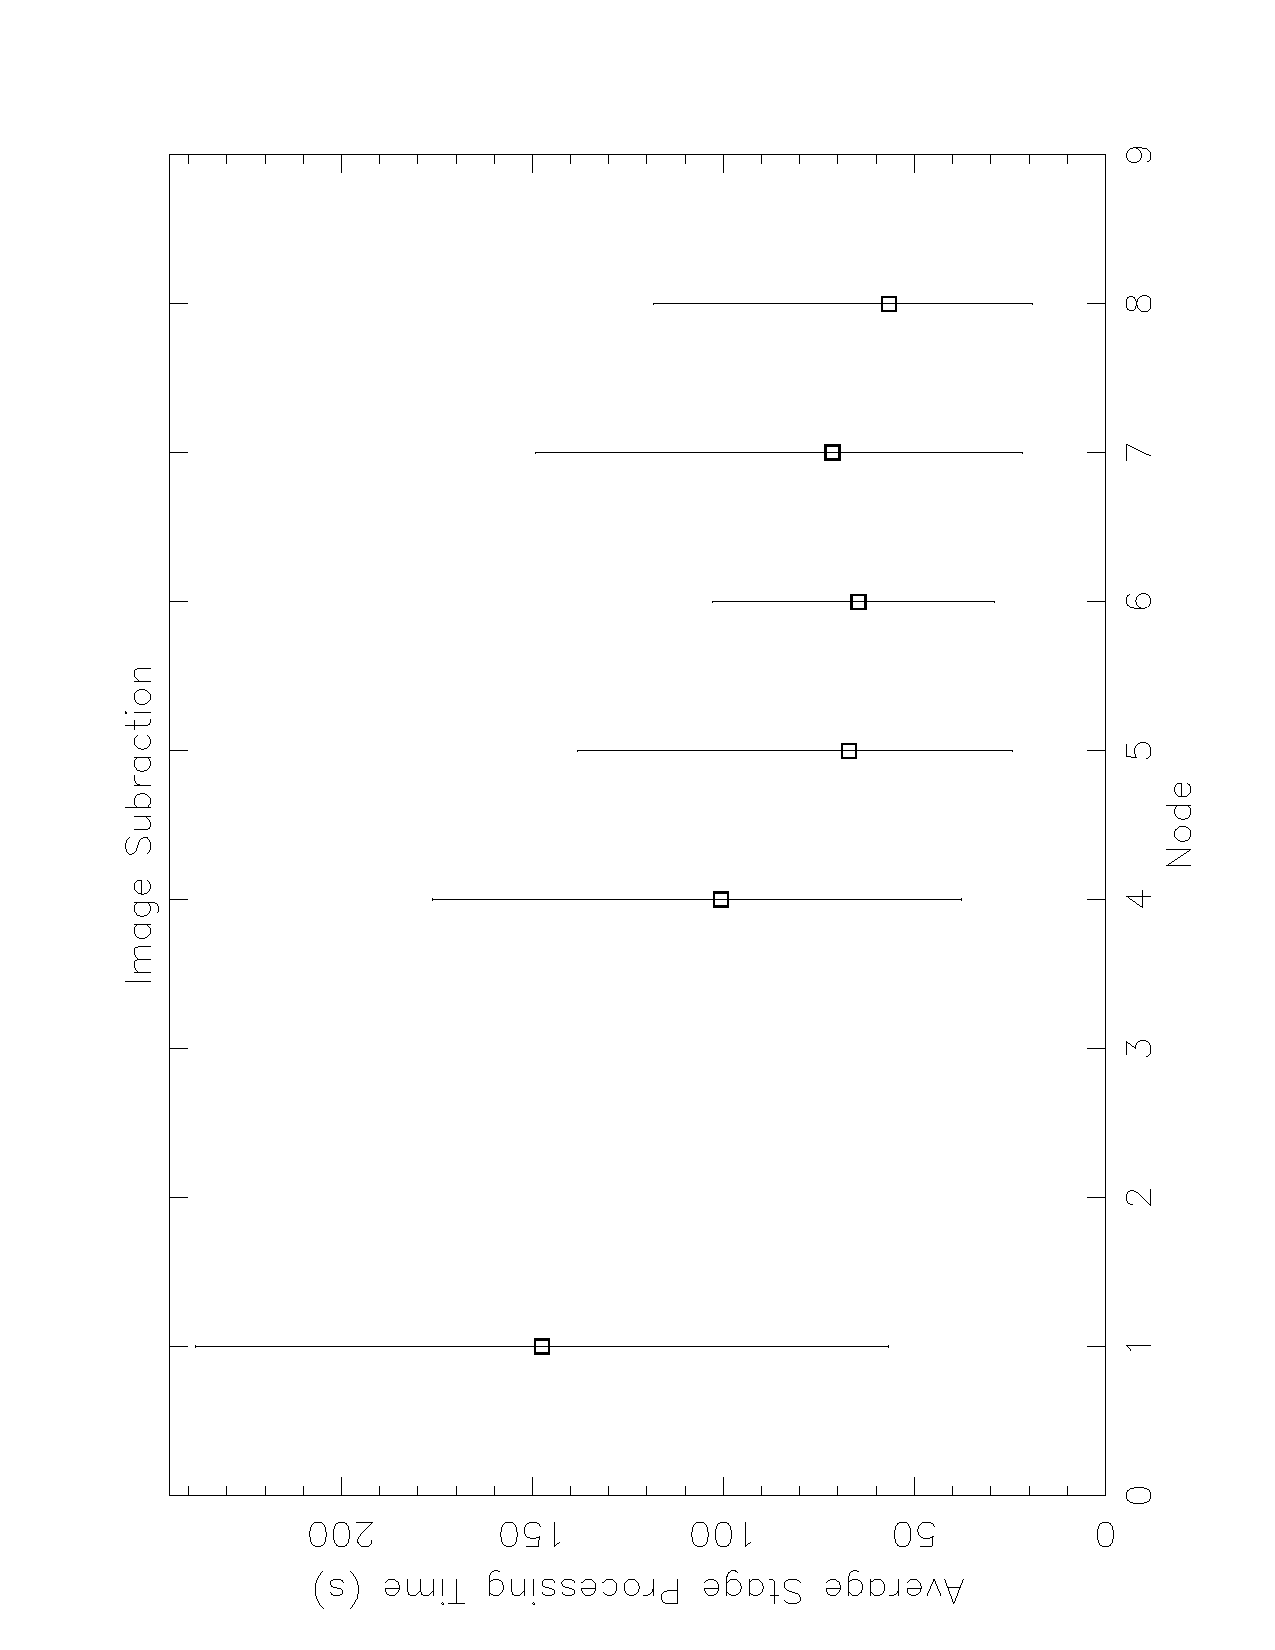
\includegraphics[width=0.8\textwidth,angle=-90,scale=0.45,viewport=59 19 572 722,clip]{figures/StageProcVsNode.pdf}
\caption{A plot of the average time (represented by the squares)
  spent within the \code{process()} step of the IPD pipline's stage 6
  as a function of node.  The bars passing through each square extend
  to the minimum and maximum times measured on that node.  Nodes 1--4
  are older, less powerful machines than nodes 5--8.
\label{average-node-time}} 

\vspace{0.5\baselineskip}

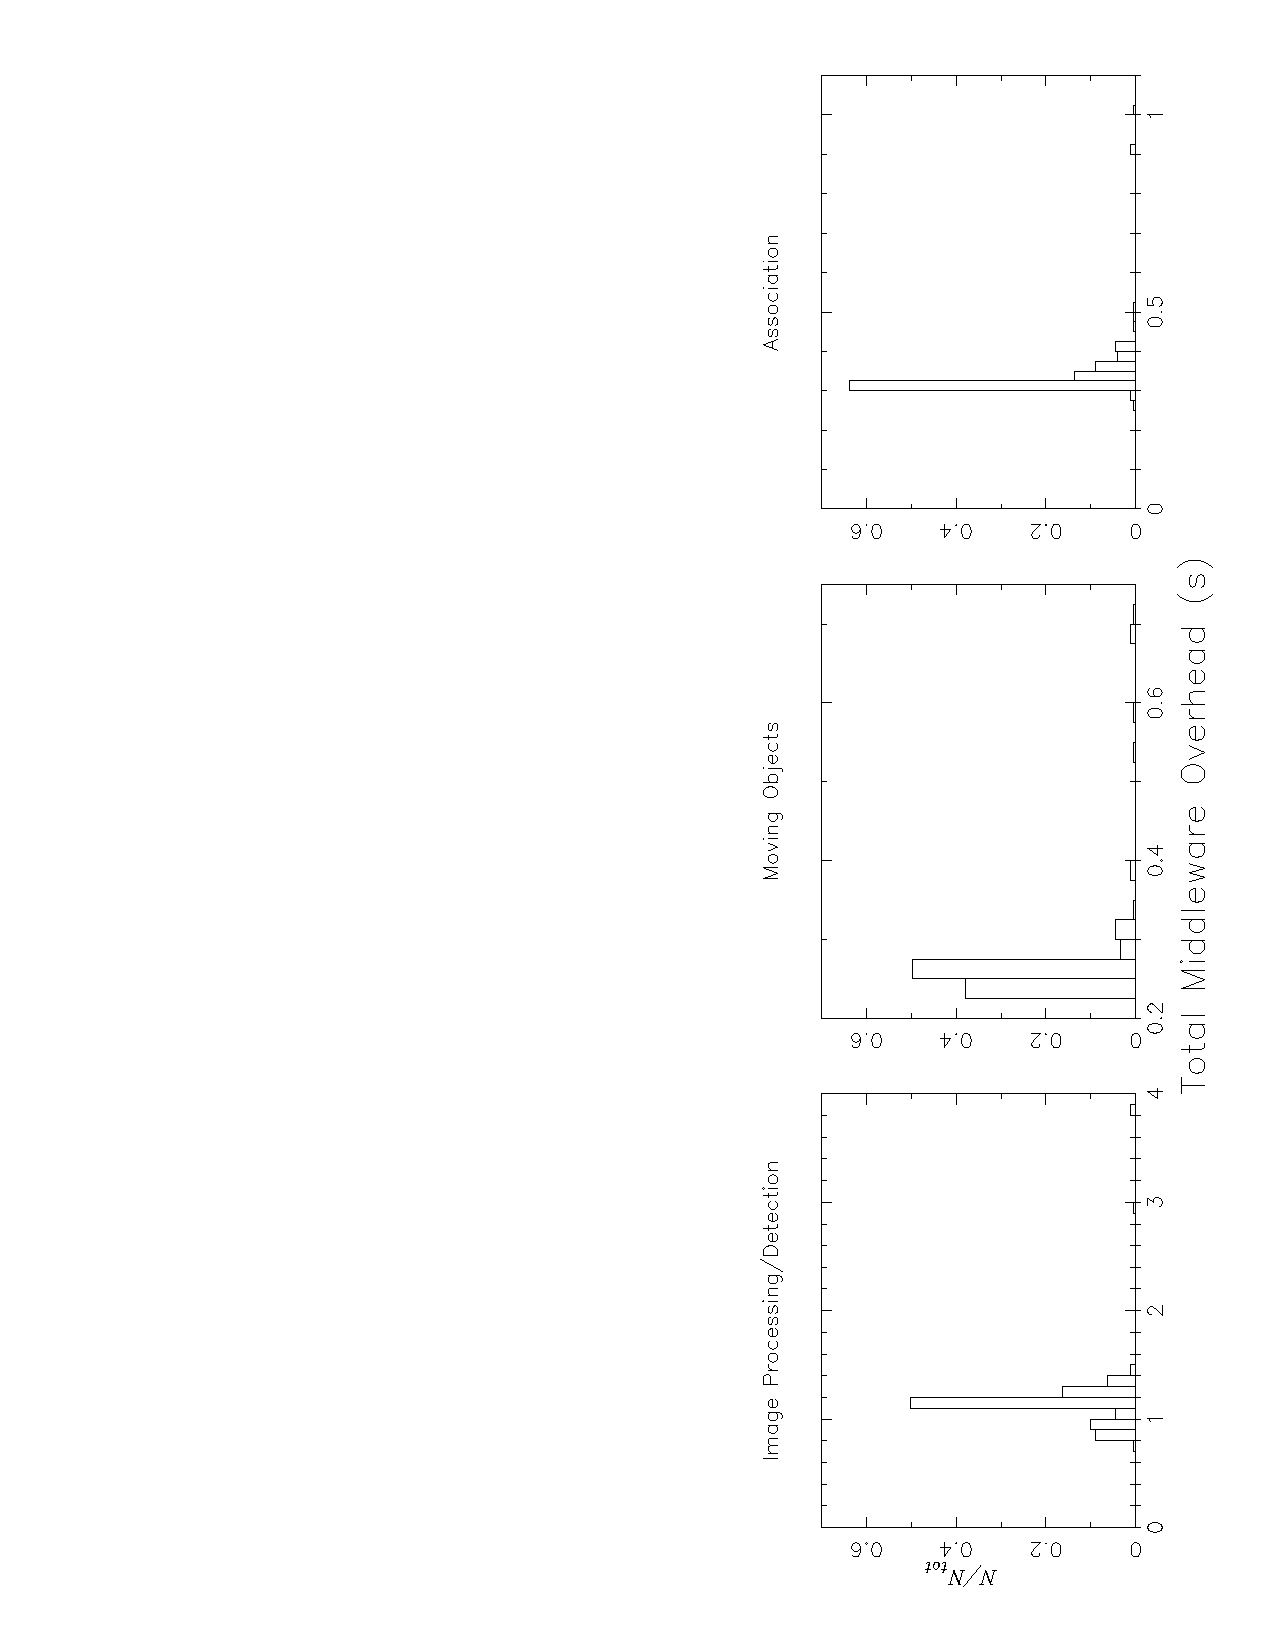
\includegraphics[width=0.8\textwidth,angle=-90,scale=0.375,viewport=364 29 583 757,clip]{figures/LoopOverhead.pdf}
\caption{Histogram of the overhead penalties --- that is, the time not
  spent in application code while processing one visit --- imposed by the pipeline
  framework.  The $y$-axis measures the fraction of the 177 visits in
  each time bin.\label{f6-7}} 

\vspace{0.5\baselineskip}

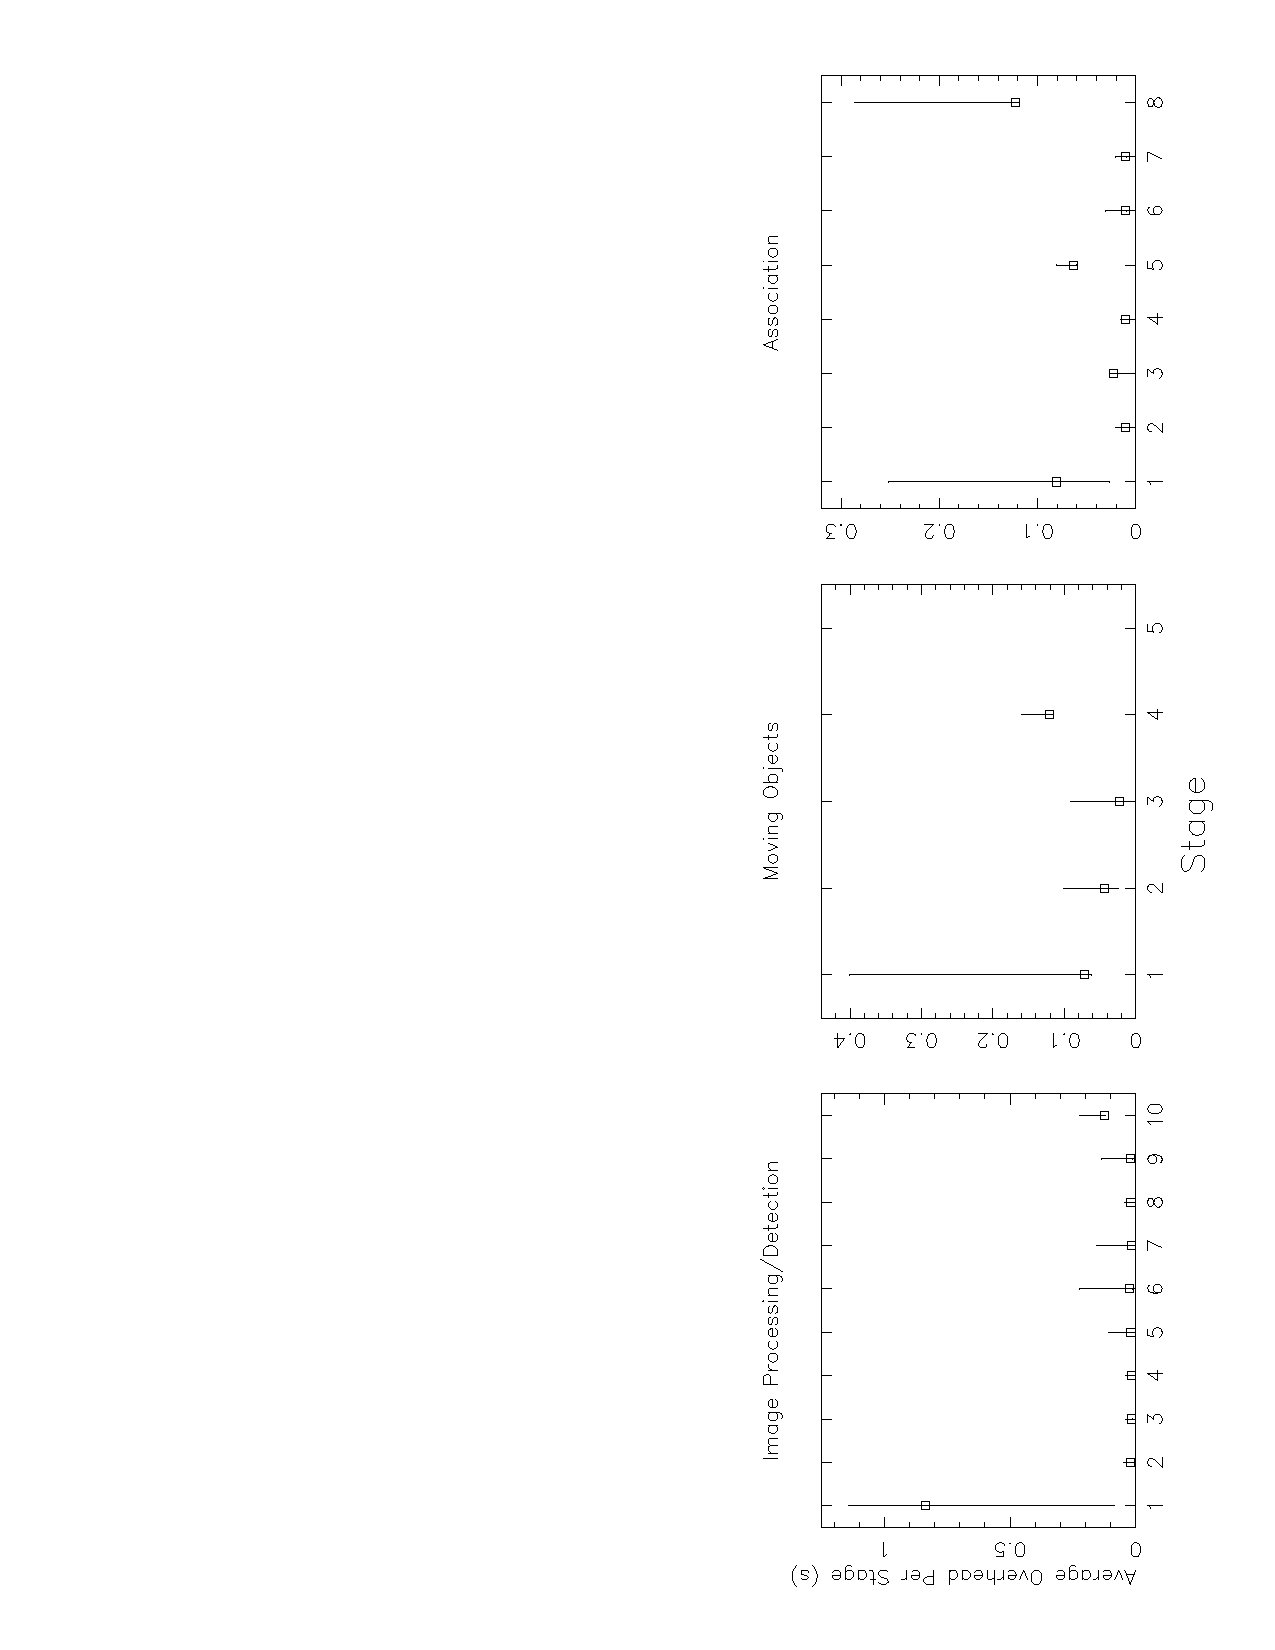
\includegraphics[width=0.8\textwidth,angle=-90,scale=0.375,viewport=364 29 583 757,clip]{figures/OverheadVsStage.pdf}
\caption{The average overhead times (represented by squares) as a
  function of stage for each pipeline.  The vertical lines through
  the squares extend to the minimum and maximum times. \label{f6-8}} 
\end{center}
\end{figure}

\begin{deluxetable}{lrr}
\tablecaption{Average overhead time per visit for each pipeline.\label{t6-4}}
\tablewidth{0pt}
\tablehead{
\colhead{Pipeline} & \colhead{avg. time (s)} & \colhead{$3\sigma$ (s)}
}
\startdata
Image Processing/Detection (IPD) &  1.17 & 1.03 \\
Moving Objects (MOPS)            &  0.27 & 0.20 \\
Association                      &  0.34 & 0.26 \\
\enddata
\\[-1.5\baselineskip]
\tablecomments{$N_{visits}=177$}
\end{deluxetable}

Because we can fairly accurately measure the time spent running actual
application code (covered in the \code{pre-process()}, \code{process()} and
\code{post-process()} steps), we can also measure the extra time that
the pipeline framework adds managing the pipeline; we refer to this as
the pipeline framework's \textit{overhead}.  Overhead is calculated on a
per visit basis, taking the total processing time for the visit (as
illustrated in \Fig{f6-4}) and subtracting the total time in
application code as well as the time spent waiting for an event to
arrive.  The averages of these overheads are summarized in
Table~\ref{t6-4} and illustrated in \Fig{f6-7}.  These results
show that the overhead is quite low (compared to the total processing
time).  \Fig{f6-7} shows that the overhead times are fairly
consistent.  \Fig{f6-8} shows how the overhead varies on
average as a function of the stage.  The overhead is larger on average
for the stages that receive events (stage 1 for all three pipelines
and stage 5 for the Association pipeline) and for the last stage after
which the clipboard must be cleaned up and restored.

\section{Conclusions}

% Tie in DC2 results to goals presented in Intro.
% Desired functionality in place
% Speed too slow, but isolated to convolution code; cause understood
% Science quality needs work - OK for DC2

We now refer back to the goals for DC2 presented in \Sec{Goals}, and
assess how they have been met.  To facilitate the discussion, it is
convenient to group the goals:

\begin{itemize}
\item Construction and demonstration of application framework and
  astronomical algorithms in the context of the LSST nightly processing pipeline.
\begin{itemize}
\item Demonstrate the use of astronomical algorithms for nightly
  processing in an LSST processing framework. 
\item Further develop and demonstrate common application framework
  functionality.
\item Establish an LSST simulated object/source database for testing
  by the broader collaboration.
\item Demonstrate integration of MOPS into LSST framework. 
\end{itemize}
\item Construct and demonstrate a middleware framework that
  supports the application framework.
\begin{itemize}
\item Update middleware implementation to enable the hosting and
  execution of application classes.
\item Demonstrate a database partitioning scheme.
\end{itemize}
\item Establish software development process that will persist through construction.
\begin{itemize}
\item Pilot the software development and testing process for future data
  challenges and the LSST construction phase.
\item Establish reusable code baseline for future data challenges and
  the LSST construction phase.
\end{itemize}
\end{itemize}

The goals for the application framework and for the algorithms implemented
using it have been nearly completely achieved, and this is clearly one of
the major results of DC2.  The prototype nightly processing pipelines
include the required algorithms, and have worked reliably as measured
by the fraction of input images that are successfully processed
through the pipeline. The one goal we have not achieved is establishing
a realistic object/source database for use by the broader collaboration.
While we have successfully implemented the database to the schema as
designed, and populated it with properly structured and linked data,
the data quality is not yet sufficient to be useful to the broader
collaboration.  The reasons for this are well understood, as discussed
in \Sec{ScienceDataQuality}, and much of the application code required
to achieve the goal has already been written and tested.

The innovation of the newly implemented pipeline harness is in the way
it effectively balances the use of Python and C++.  Application
Stages --- the container for the scientific algorithms --- can be written
with ease in Python.  These stage implemenations themselves can be
thin wrappers around our C++ classes.  Similarly, the pipeline harness
itself is a wrapper around a C++ implementation where the MPI control
calls are executed.  Our timing results show that the overhead added to
the total processing time by the pipeline harness is very small
compared to application processing time.  In particular, the overhead
scales linearly with the number of stages ($< 0.1$ seconds per stage) in
the absence of event processing.  Sending and receiving events adds
additional but still small overhead.  

Our pipeline harness does have a disadvantage that becomes apparent
when run on a heterogeneous cluster as we did.  Because of the way we
synchronize our processing, the overall speed of the pipeline is
limited by the performance of the slowest node.  This is important to
consider for the production system.  When we scale up to hundreds or
even thousands of cores and run nearly 24 hours a day, one or two
defective nodes could easily bring down the performance of the entire
cluster.  In future data challenges, we will look at strategies for
not only minimizing this effect, but also detecting when defective
nodes are having a major impact on performance.  

We have been quite successful in building up an effective software
development environment that not only builds the software via a few
simple commands but also manages all of the dependencies.  The ability
to have multiple versions of a package simultaneously, as provided by
the EUPS system, has been a very powerful feature, particularly during
the integration phase when many changes were coming in rapidly.  

Our package distribution system has also been an important mechanism
for our distributed team to keep up with the latest changes.  However,
the distribution system has suffered from two serious problems.  The first
has been in ensuring smooth installation of third party packages
across all of our development platforms.  While the differences
between the Mac and Linux platforms has been most challenging
(particularly for certain ``problem'' packages like Boost, CORAL, and
SEAL), supporting different distributions of Linux (particularly
64-bit Linux) has not been without problems.  Cross-platform support
issues for third-party packages have been the most common problem that
has prevented developers from getting the software stack installed on
their local environment.  The second problem stems from the amount of
time it takes to install a full software stack (as we build everything
from source).  This is not only a barrier to new developers but to
those of us who maintain the build and distribution system as it makes
debugging platform-dependent problems a slow process.  We hope our
future experiments with virtual machines will alleviate the barrier
for new developers.  

One observation that we have drawn from these problems is that
when the build environment runs well, the developer hardly notices it.
When it doesn't work, it can quickly disable a developer's progress.

\subsection{Required software developments for DC3}

As we prepare to transition from the completion of DC2 to the
development of DC3, it is appropriate to assess what improvements will
be required in the existing LSST software.  First, we emphasize that
our experience with the DC2 framework, and with the software
development system with which it was designed, built, and documented,
has been very positive.  We will use it as the foundation for DC3.

As we fully expected, however, we will need to extend it in various ways. The
preceding sections of this report have identified a number of detailed
improvements to the existing framework classes that we expect to need
for DC3.  We will not recap those here, rather taking a somewhat
higher level view.  The main required developments that we have
identified are:

\begin{itemize}

\item We need to define the role of the middleware orchestration layer in
   catching exceptions and possibly mediating adaptive behavior of the
   pipeline stages in recovering from problems such as algorithmic
   failures.

\item Need to define API and mechanism for inter-slice communication (not
   present or required for DC2).  We
   have at least three usecases that require some form of inter-slice
   communication: cross-talk correction; the association pipeline (which
   is currently using shared memory outside of the pipeline framework
   for this), and handling Footprints that cross amplifier boundaries

\item Related to inter-slice communication, the LSST focalplane, with
   its roughly 3000 amplifiers, 200 ccds, and 21 rafts, has lots of
   boundaries. We need to carefully assess where processing needs to take account of
   what's on the other side of a boundary.

\item We need to address the performance issues with accessing pixels
   under vw.  This is the source of our only significant performance problem.

\item We need to further develop the image subtraction software to
improve the data quality of the subtracted images.

\end{itemize}

\subsection{Scaling to LSST}

Finally, we need to assess where we stand in relation to the final
performance requirements for LSST.  The input images we have used for
DC2 have 340 Megapixels, just over 10\% the size of the LSST
focalplane.  They also have very similar pixel scale and somewhat
greater exposure depth as a single LSST exposure.  Although the
hardware available for DC2 prevented us from processing full images in
parallel, the DC2 software is designed to do so without modification.
We expect to make such runs shortly after completion of this report.
We are thus very close to processing a data stream that is 10\% that
of LSST.  This is in line with the expectations for DC2 set in the
MREFC proposal.

We do have a significant shortfall in the per-node performance on the
nightly processing pipeline, achieving about 20\% of what is required
to meet the 60 sec alert processing latency.  As discussed above, we
believe that we have isolated the performance problem to a small
section of code that utilizes the vw library (see \Sec{fwTiming}) to access image
pixels. Our strategy for verifying that we are on track to achieve the full LSST
performance level is to:

\begin{itemize}
\item Complete the full focalplane DC2 runs, utilizing 288 nodes for
  the IPD pipeline.  This will verify that the middleware framework is
  not limiting performance.
\item Work with the vw group at NASA Ames to resolve the pixel access
  performance issues that are limiting image subraction speed.
\item In the event that vw continues to be a performance issue, we
  will replace it.  The application APIs would not be significantly
  impacted by such a change, so changes to the existing software stack
  would be very localized.
\item As a risk reduction strategy, we will continue our ongoing
  effort to track and evaluate the performance of GPU and related
  architectures for image processing tasks.  Based on present
  application experience, these offer at least a factor of 4
  improvement in per-node performance, which gives ample headroom to
  meet full LSST performance.
\item We need to address load balancing issues inherent to our
  pipeline harness to ensure that a few defective nodes in a cluster
  do not drag down the performance of a massively parallel pipeline.  
\end{itemize}

We will have results from the first three steps in this plan by May, 2008.




\end {document}
